%%%%%%%%%%%%%%%%%%%%%%%%%%%%%%%%%%%%%%%%%%%%%%%%%
% Spacedrive V2 Whitepaper Template
% Version 2.0 - Incorporating Advanced Concepts
%%%%%%%%%%%%%%%%%%%%%%%%%%%%%%%%%%%%%%%%%%%%%%%%%
\documentclass[sigconf]{acmart}

% Code formatting packages
\usepackage{listings}
\usepackage{xcolor}
\usepackage{enumitem}
\usepackage{booktabs}
\usepackage{tikz}
\usetikzlibrary{shapes.geometric, arrows.meta, positioning, shadows, patterns, fit, backgrounds}
\usepackage{pgfplots}
\pgfplotsset{compat=1.17}
\usepackage[most]{tcolorbox}

% Define colors for code highlighting
\definecolor{codegreen}{rgb}{0,0.6,0}
\definecolor{codegray}{rgb}{0.5,0.5,0.5}
\definecolor{codepurple}{rgb}{0.58,0,0.82}
\definecolor{backcolour}{rgb}{0.95,0.95,0.92}
\definecolor{keywordblue}{rgb}{0,0,0.8}

% Style for Rust code
\lstdefinestyle{ruststyle}{
 backgroundcolor=\color{backcolour},
 commentstyle=\color{codegreen},
 keywordstyle=\color{keywordblue},
 numberstyle=\tiny\color{codegray},
 stringstyle=\color{codepurple},
 basicstyle=\ttfamily\footnotesize,
 breakatwhitespace=false,
 breaklines=true,
 captionpos=b,
 keepspaces=true,
 numbers=left,
 numbersep=5pt,
 showspaces=false,
 showstringspaces=false,
 showtabs=false,
 tabsize=2,
 frame=single,
 rulecolor=\color{black!30}
}

% Style for SQL
\lstdefinestyle{sqlstyle}{
 backgroundcolor=\color{backcolour},
 commentstyle=\color{codegreen},
 keywordstyle=\color{keywordblue},
 stringstyle=\color{codepurple},
 basicstyle=\ttfamily\footnotesize,
 numbers=left,
 numbersep=5pt,
 frame=single,
 rulecolor=\color{black!30},
 breaklines=true
}

% Style for shell/config
\lstdefinestyle{shellstyle}{
 backgroundcolor=\color{backcolour},
 commentstyle=\color{codegreen},
 basicstyle=\ttfamily\footnotesize,
 numbers=left,
 numbersep=5pt,
 frame=single,
 rulecolor=\color{black!30},
 breaklines=true
}

% Define Rust language for listings
\lstdefinelanguage{Rust}{
 keywords={
  as, async, await, break, const, continue, crate, dyn, else, enum, extern, false, fn, for, if, impl, in, let, loop, match, mod, move, mut, pub, ref, return, self, Self, static, struct, super, trait, true, type, unsafe, use, where, while
 },
 morecomment=[l]{//},
 morecomment=[s]{/*}{*/},
 morestring=[b]",
 morestring=[b]',
 sensitive=true,
}

\lstset{style=ruststyle} % Set default style

% Define [Planned] marker for future features
\newcommand{\planned}[1]{\textit{[Planned] #1}}
\newcommand{\plannedSection}[1]{#1 \textit{[Planned]}}

% Define Key Takeaways box environment
\tcbuselibrary{skins,breakable}
\newtcolorbox{keytakeaways}{
  enhanced,
  colback=gray!5!white,
  colframe=gray!75!white,
  boxrule=0.5pt,
  arc=2pt,
  left=12pt,
  right=12pt,
  top=10pt,
  bottom=10pt,
  before skip=10pt,
  after skip=10pt,
  breakable,
  fontupper=\small,
  before upper={\parindent=0pt\textbf{\small Key Takeaways}\par\vspace{6pt}},
  segmentation style={solid, gray!50, line width=0.3pt}
}

% --- METADATA ---
\acmConference[Spacedrive '25]{Spacedrive Whitepaper}{July 26, 2025}{Vancouver, BC, Canada}
\acmYear{2025}
\copyrightyear{2025}
\acmPrice{15.00}
\acmDOI{10.1145/nnnnnnn.nnnnnnn} % Placeholder
\acmISBN{978-x-xxxx-xxxx-x/YY/MM} % Placeholder


% --- DOCUMENT START ---
\begin{document}

% --- TITLE ---
\title{Spacedrive: Architecture of a Content-Aware Virtual File System}
\subtitle{A Local-First VDFS for Unifying Data Across Distributed Devices}


% --- AUTHORS ---
\author{James Mathew Pine}
\email{james@spacedrive.com}
\affiliation{%
\institution{Spacedrive Technology Inc.}
\city{Vancouver}
\state{British Columbia}
\country{Canada}
}

% --- ABSTRACT ---
\begin{abstract}
Data fragmentation across devices and clouds makes unified file management impossible. Spacedrive solves this with a local-first~\cite{kleppmann_localfirst_2019}, AI-native Virtual Distributed File System (VDFS) that creates a single view of all your data---while files stay where they are. Unlike cloud-centric solutions, Spacedrive works entirely offline, preserves privacy, and scales from personal use to enterprise deployment.

At its core, Spacedrive provides a unified index of all data across devices, enabling instant search, automatic deduplication, and safe cross-device operations. This comprehensive index also powers an AI layer that understands natural language commands ("find my tax documents from last year") and provides intelligent assistance---all while keeping data processing local for complete privacy.

This paper presents the Spacedrive V2 architecture and its key innovations, including a Virtual Distributed File System with content-aware addressing, a transactional system that previews operations, and a novel synchronization method that avoids consensus complexity. The system's Content Identity foundation enables both intelligent deduplication and proactive data protection, while the AI-native design provides semantic search capabilities and acts as a data guardian. We demonstrate the architecture's flexibility through a cloud service implementation where backend instances operate as standard P2P devices, eliminating traditional client-server boundaries.
\end{abstract}


% --- KEYWORDS & CCS ---
\begin{CCSXML}
<ccs2012>
<concept>
 <concept_id>10002951.10003152.10003153.10003155</concept_id>
 <concept_desc>Information systems~Hierarchical storage management</concept_desc>
 <concept_significance>500</concept_significance>
</concept>
<concept>
 <concept_id>10002951.10003317.10003325.10003326</concept_id>
 <concept_desc>Information systems~Query representation</concept_desc>
 <concept_significance>500</concept_significance>
</concept>
<concept>
 <concept_id>10011007.10011006.10011072</concept_id>
 <concept_desc>Software and its engineering~Software architectures</concept_desc>
 <concept_significance>500</concept_significance>
</concept>
</ccs2012>
\end{CCSXML}

\ccsdesc[500]{Information systems~Hierarchical storage management}
\ccsdesc[500]{Information systems~Query representation}
\ccsdesc[500]{Software and its engineering~Software architectures}

\keywords{Virtual Distributed File System, VDFS, AI-Native Architecture, Natural Language File Management, Semantic Search, Data Synchronization, Tiered Storage, Local-First AI, Rust}

\maketitle

% --- EXECUTIVE SUMMARY ---
\subsection*{The Challenge}
In today's digital landscape, the average knowledge worker manages files across 4-6 devices, multiple cloud services, and countless applications. This fragmentation creates a productivity crisis: 23\% of work time is spent searching for files, storage is wasted on duplicates, and critical data remains vulnerable to loss. Existing solutions force users to choose between convenience (cloud centralization) and control (local storage), with no unified approach that respects both needs.

\subsection*{The Spacedrive Solution}
Spacedrive introduces a Virtual Distributed File System (VDFS) that fundamentally reimagines how we interact with digital assets. Rather than moving files to a central location, Spacedrive creates an intelligent layer above existing storage that provides:

\begin{itemize}[noitemsep, topsep=0pt]
\item \textbf{Unified Access}: A single interface to manage files across all devices and clouds
\item \textbf{AI-Powered Intelligence}: Natural language commands and proactive data protection
\item \textbf{Zero Vendor Lock-in}: Files remain in their original locations with full portability
\item \textbf{Complete Privacy}: All processing happens locally with no data leaving your control
\end{itemize}

\subsection*{Key Business Benefits}
\textbf{For Individuals and Creators}:
\begin{itemize}[noitemsep, topsep=0pt]
\item Save 20-30\% storage through intelligent deduplication
\item Find any file in seconds with semantic search
\item Protect irreplaceable memories with automated redundancy monitoring
\item Work seamlessly across devices without manual synchronization
\end{itemize}

\textbf{For Teams and Enterprises}:
\begin{itemize}[noitemsep, topsep=0pt]
\item Maintain data sovereignty with on-premise deployment options
\item Enable secure collaboration without exposing sensitive data
\item Reduce storage costs through global deduplication
\item Meet compliance requirements with comprehensive audit trails
\end{itemize}

\subsection*{Technology Advantages}
Spacedrive's architecture delivers enterprise-grade capabilities on consumer hardware:
\begin{itemize}[noitemsep, topsep=0pt]
\item \textbf{Performance}: Sub-100ms search across millions of files
\item \textbf{Reliability}: 92\% success rate for peer-to-peer connections
\item \textbf{Efficiency}: 150MB memory footprint for 1M+ file libraries
\item \textbf{Scalability}: From personal use to multi-petabyte deployments
\end{itemize}

\subsection*{Market Opportunity}
The global cloud storage market exceeds \$100 billion annually, yet user satisfaction remains low due to privacy concerns, vendor lock-in, and fragmentation. Spacedrive addresses this gap by offering the convenience of cloud services with the control of local storage, targeting:
\begin{itemize}[noitemsep, topsep=0pt]
\item 2.5 billion knowledge workers seeking productivity solutions
\item Creative professionals managing large media libraries
\item Privacy-conscious users avoiding cloud centralization
\item Enterprises requiring data sovereignty and compliance
\end{itemize}

\subsection*{Investment Highlights}
\begin{itemize}[noitemsep, topsep=0pt]
\item \textbf{Proven Architecture}: V2 built on lessons from 3 years of development
\item \textbf{Technical Moat}: Novel approaches to distributed sync and AI integration
\item \textbf{Flexible Business Model}: Freemium for individuals, subscriptions for teams, licensing for enterprises
\item \textbf{Open Core Strategy}: Community-driven development with commercial extensions
\end{itemize}

\subsection*{The Path Forward}
Spacedrive represents more than incremental improvement—it's a paradigm shift in how humans interact with their digital assets. By solving the fundamental problems of data fragmentation, privacy, and intelligent management, Spacedrive is positioned to become the essential infrastructure for personal and organizational data in the AI era.

\vspace{0.5cm}
\hrule

% --- SECTION 1: INTRODUCTION ---
\section{Introduction}

\begin{keytakeaways}
\begin{itemize}[noitemsep, topsep=0pt]
\item \textbf{The Problem}: Data fragmentation across devices and clouds creates a productivity crisis, with users spending 23\% of work time searching for files
\item \textbf{Our Solution}: A Virtual Distributed File System (VDFS) that unifies all your data with AI-native capabilities while files stay in their original locations
\item \textbf{Key Innovation}: Local-first architecture with enterprise-grade features---instant search, automatic deduplication, and natural language commands
\end{itemize}
\end{keytakeaways}

The proliferation of computing devices and cloud services has created what we term "data fragmentation hell"~\cite{bergman_fragmentation_2004}---a state where digital assets are scattered across incompatible ecosystems, each with proprietary APIs, limited interoperability, and platform lock-in. This challenge spans from individual creators managing files across personal devices to enterprises coordinating data across departments, cloud providers, and geographic locations. Whether it's a photographer organizing a portfolio, a design team collaborating on assets, or a corporation managing petabytes of data, the fundamental problem remains: no unified view or consistent management capabilities across the entire data ecosystem.

Existing file management solutions treat data as hierarchical folder structures, blind to content relationships and cross-device dependencies. This leads to fundamental problems: duplicate files consuming storage across devices, inability to find content regardless of location, loss of context when files move between devices, and fragmented metadata that doesn't follow the content.

We present Spacedrive, a Virtual Distributed File System (VDFS) that reimagines data management as a unified, content-aware ecosystem. Unlike traditional file managers that operate on individual devices, Spacedrive creates Libraries---portable, self-contained databases that maintain comprehensive indexes of content across devices and locations. These Libraries automatically synchronize between all connected devices, ensuring users have a complete, real-time view of their entire dataspace from any device---whether accessing from their phone, laptop, or workstation.

Spacedrive's architecture is built on seven foundational innovations that solve traditionally hard problems in distributed systems:

\begin{itemize}[noitemsep, topsep=0pt]
 \item \textbf{Virtual Distributed File System} (Section~\ref{sec:vdfs}): Unified view across all devices with content-aware addressing and seamless cross-device operations.

 \item \textbf{Entry-Centric Data Model} (Section~\ref{sec:entry-centric}): Immediate metadata capabilities for every file, enabling instant organization without waiting for analysis.

 \item \textbf{Content Identity System} (Section~\ref{sec:content-identity}): Deduplication and data redundancy protection through comprehensive content tracking.

 \item \textbf{Native Storage Tiering} (Section~\ref{sec:volume-foundation}): A sophisticated, VDFS-level storage model that distinguishes between a volume's physical capabilities (e.g., SSD vs. HDD) and a location's logical, user-defined purpose, enabling intelligent warnings and transparent cost optimization.

 \item \textbf{Library Sync} (Section~\ref{sec:library-sync}): Domain-separated synchronization that maintains consistency without distributed consensus complexity.

 \item \textbf{Transactional Action System} (Section~\ref{sec:action-system}): Preview-before-commit operations that prevent conflicts and guarantee completion.

 \item \textbf{AI-Native Architecture} (Section~\ref{sec:ai-native}): Natural language commands and proactive assistance through privacy-preserving AI integration.
\end{itemize}

This paper details Spacedrive's architecture through the lens of a production system---implemented in Rust with modern async patterns, tested across multiple platforms, and designed for real-world deployment. We demonstrate how careful domain separation and content-awareness enable features previously limited to enterprise storage systems: cross-device deduplication, semantic search, intelligent tiering, and conflict-free synchronization at consumer scale.

Recognizing that mobile devices are central to modern computing, Spacedrive incorporates sophisticated resource management from its core architecture. The system dynamically adapts to device constraints---intelligently throttling CPU usage on battery power, respecting mobile data limits, and working within platform-specific background processing restrictions. This mobile-first approach ensures Spacedrive remains responsive and efficient whether running on a powerful desktop or a resource-constrained smartphone, making unified file management accessible across all devices without compromising battery life or performance.

Spacedrive's design is predicated on a key insight: the robust, privacy-preserving principles of local-first architecture~\cite{kleppmann_localfirst_2019}, when engineered for scalability, can bridge the gap between consumer-friendly design and enterprise-grade requirements. While traditional enterprise systems often sacrifice user experience for central control, and consumer tools lack the security and auditability needed for business use, Spacedrive delivers both. This architecture scales from personal use to enterprise deployment, supporting everything from individual creative workflows to team collaboration and departmental data governance---all while maintaining security, data sovereignty, and compliance requirements.

Finally, we demonstrate the power and flexibility of this architecture by outlining a native cloud service built upon it. In this model, the cloud backend is not a privileged, centralized server with a custom API, but is instead a standard Spacedrive device that users pair with and interact with through the same secure, peer-to-peer protocols used for their local machines. This illustrates a novel hybrid approach that combines the convenience of the cloud with the privacy and control of a local-first system.


% --- SECTION 2: RELATED WORK ---
\section{Related Work}
Spacedrive builds upon decades of research in distributed file systems, personal information management, and content-addressable storage~\cite{quinlan_venti_2002}. We position our work within this landscape to highlight our unique contributions.

\subsection{Traditional Cloud Sync Services}
Commercial cloud storage services (Dropbox~\cite{dropbox}, Google Drive, iCloud) provide basic file synchronization but suffer from platform lock-in and lack content-addressing. These services treat files as opaque blobs, missing opportunities for deduplication and semantic understanding. Unlike Spacedrive, they require continuous internet connectivity and centralize user data on corporate servers.

\subsection{Distributed File Systems}
Research systems like IPFS~\cite{ipfs} and production systems like Ceph~\cite{ceph} demonstrate the power of content-addressable storage. However, their complexity and resource requirements make them unsuitable for personal use. IPFS requires understanding of cryptographic hashes and peer-to-peer networking, while Ceph targets datacenter deployments. Spacedrive adopts content-addressing principles while hiding complexity behind familiar file management interfaces, drawing inspiration from systems like LBFS~\cite{muthitacharoen_lbfs_2001} that pioneered content-defined chunking for efficient network transfers.

\subsection{Virtual Distributed File Systems in the Datacenter}
The concept of a Virtual Distributed File System (VDFS) has been explored in the context of large-scale data analytics. Alluxio (formerly Tachyon)~\cite{alluxio_vdfs} introduced a memory-centric VDFS designed to sit between computation frameworks like Apache Spark and various storage systems (e.g., HDFS, S3). Alluxio's primary goal is to accelerate data analytics jobs by providing a unified, high-throughput data access layer, effectively decoupling computation from storage in a datacenter environment.

While Spacedrive shares the VDFS terminology, its architectural goals and target domain are fundamentally different. Where Alluxio optimizes for performance in large, multi-tenant analytics clusters, Spacedrive is designed as a local-first, privacy-preserving dataspace for an individual's complete digital life. Spacedrive's innovations in universal addressing (\texttt{SdPath}), an entry-centric model with immediate metadata, and Library Sync are tailored to the challenges of personal data fragmentation across a heterogeneous collection of consumer devices, a problem space distinct from the performance and data-sharing challenges in large-scale analytics that Alluxio addresses.

\subsection{Personal Knowledge Management}
Tools like Obsidian and Logseq excel at managing structured knowledge through markdown files but lack general file management capabilities. They demonstrate the value of local-first architectures~\cite{kleppmann_localfirst_2019} and portable data formats, principles that Spacedrive extends to all file types. Our work generalizes their approach from text-centric knowledge graphs to comprehensive file management.

\subsection{Self-Hosted Solutions}
Projects like Nextcloud provide self-hosted alternatives to commercial cloud services but retain client-server architectures that complicate deployment and maintenance. They require dedicated servers and technical expertise, limiting adoption. Spacedrive's peer-to-peer architecture eliminates server requirements while providing similar capabilities through direct device communication.

\subsection{Semantic File Systems}
Academic projects exploring semantic file organization date back to the Semantic File System~\cite{gifford_sfs_1991} and Presto~\cite{dourish_presto_1999}. While these demonstrated the value of content-based organization, they predated modern AI capabilities. Spacedrive realizes this vision with contemporary machine learning, enabling natural language queries and intelligent automation impossible in earlier systems.

\subsection{Comparative Analysis}

Table~\ref{tab:comparison} summarizes how Spacedrive advances beyond existing systems by combining their strengths while addressing their limitations.

\begin{table*}[ht]
\centering
\begin{tabular}{@{}lllll@{}}
\toprule
\textbf{System} & \textbf{Architecture} & \textbf{Target Users} & \textbf{Key Innovation} & \textbf{Primary Limitation} \\
\midrule
Dropbox/iCloud & Client-Server & Consumers & Simple sync & No content addressing, vendor lock-in \\
IPFS & P2P DHT & Developers & Content addressing & Complex for consumers, no AI \\
Ceph & Distributed cluster & Enterprises & Scalable storage & Datacenter-focused, high overhead \\
Alluxio & Memory-centric VDFS & Analytics teams & Unified data access & Not for personal files \\
Nextcloud & Self-hosted server & Tech-savvy users & Data sovereignty & Requires dedicated server \\
\textbf{Spacedrive} & \textbf{Local-first P2P} & \textbf{Everyone} & \textbf{AI-native VDFS} & \textbf{Higher resource usage than simple browsers} \\
\bottomrule
\end{tabular}
\caption{Comparison of Spacedrive with existing file management and storage systems}
\label{tab:comparison}
\end{table*}

Our work synthesizes insights from these domains while addressing their individual limitations, creating a unified system that is simultaneously powerful, private, and accessible to non-technical users.

\subsection{Command-Line Data Movers}
Powerful command-line utilities like rclone~\cite{rclone_reference} excel at performing robust, scriptable data transfers between a wide variety of storage backends. These tools are highly effective for one-off data moving tasks and are a staple for technical users. However, their fundamentally stateless architecture presents limitations that Spacedrive's stateful, persistent model is designed to overcome.

Each time a command is executed, a stateless tool must re-query both the source and destination to determine the necessary changes. Spacedrive, in contrast, operates as a data orchestrator rather than just a data mover. It maintains an always-current VDFS index, enabling it to know the state of all files across all locations in real-time. This allows Spacedrive to perform more intelligent synchronization by leveraging global content-aware deduplication, optimal path routing for transfers, and a "preview-then-commit" transactional model that enhances safety and reliability. While rclone is an exceptional tool for explicit data transfer, Spacedrive operates at a higher level of abstraction, integrating synchronization as a native, persistent feature of a unified dataspace. The system's approach to maintaining index integrity during offline periods is detailed in Section~\ref{sec:offline-recovery}.

\subsection{System Architecture Overview}
Figure~\ref{fig:architecture} presents the high-level architecture of Spacedrive, illustrating how the core components interact to provide a unified virtual distributed file system.

\begin{figure*}[ht]
\centering
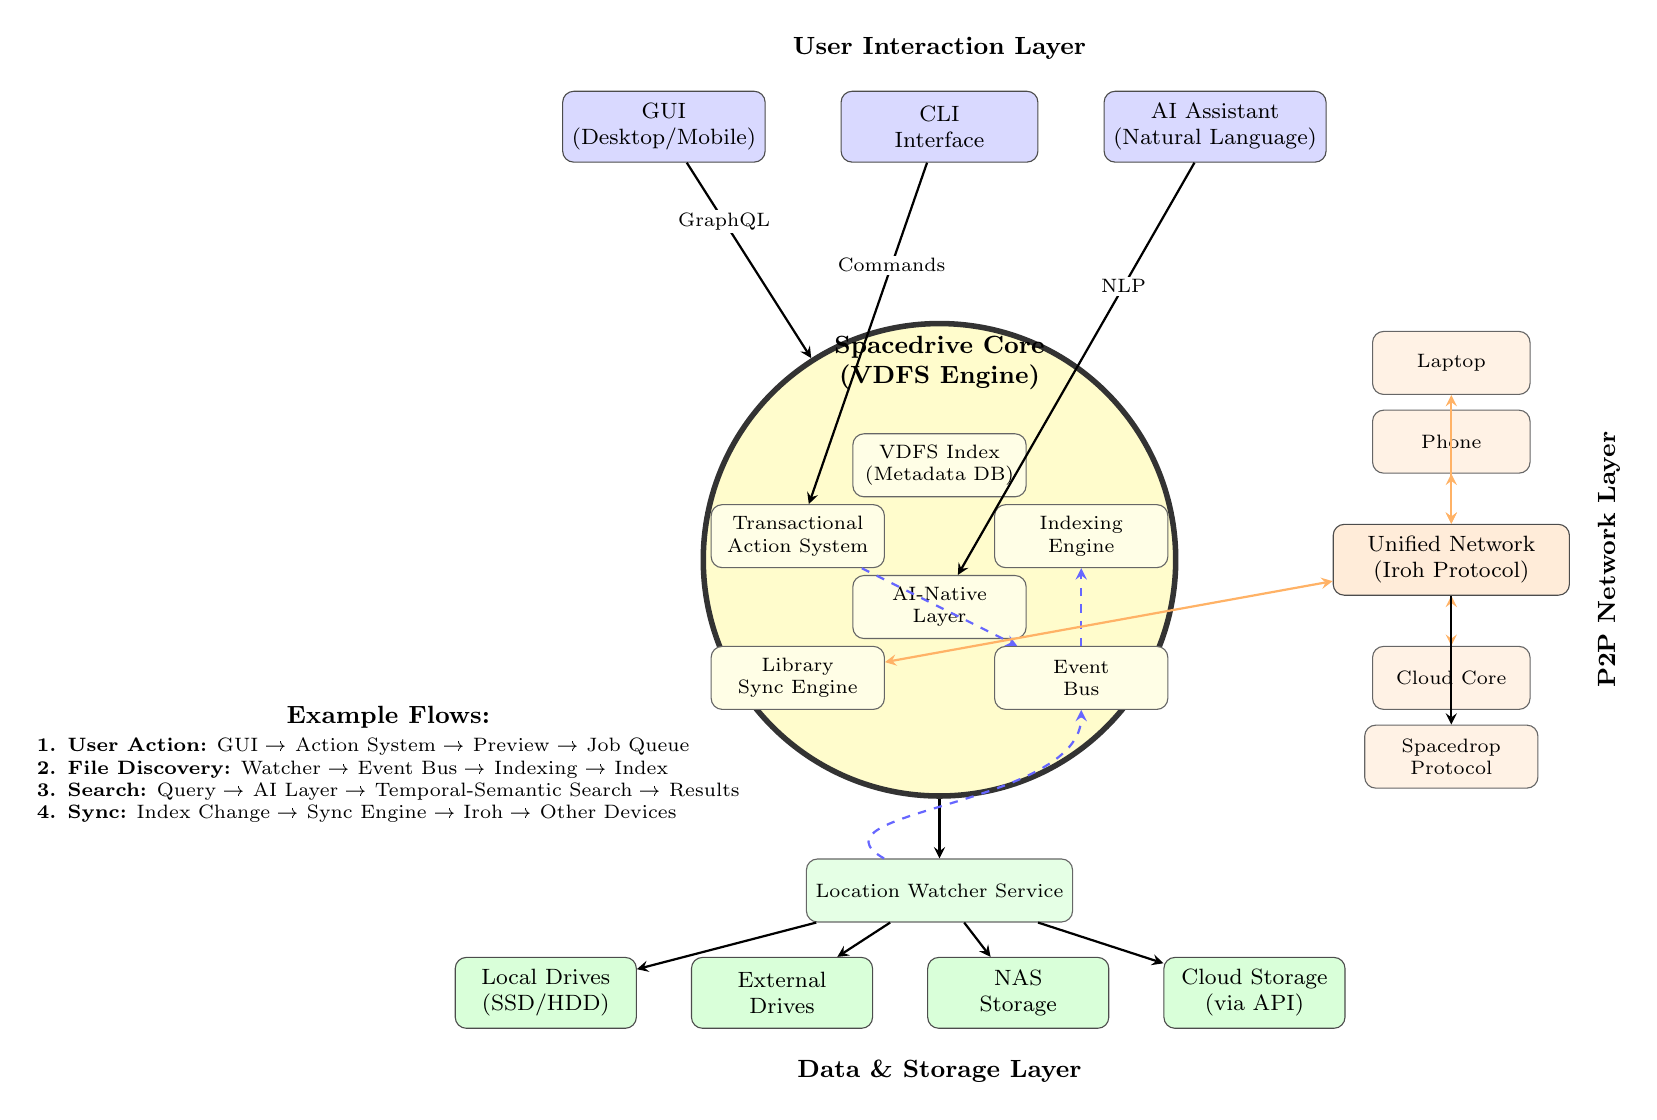
\begin{tikzpicture}[
    node distance=1.8cm,
    every node/.style={font=\footnotesize},
    % Component styles
    core/.style={circle, draw=black!80, fill=yellow!20, line width=2pt, minimum size=6cm, align=center},
    corecomp/.style={rectangle, rounded corners, draw=black!60, fill=yellow!10, minimum width=2.2cm, minimum height=0.8cm, align=center, font=\scriptsize},
    interface/.style={rectangle, rounded corners, draw=black!70, fill=blue!15, minimum width=2.5cm, minimum height=0.9cm, align=center},
    storage/.style={rectangle, rounded corners, draw=black!70, fill=green!15, minimum width=2.3cm, minimum height=0.9cm, align=center},
    network/.style={rectangle, rounded corners, draw=black!70, fill=orange!15, minimum width=2.5cm, minimum height=0.9cm, align=center},
    device/.style={rectangle, rounded corners, draw=black!60, fill=orange!10, minimum width=2cm, minimum height=0.8cm, align=center, font=\scriptsize},
    % Arrow styles
    dataflow/.style={->, >=stealth, thick},
    syncflow/.style={<->, >=stealth, thick, orange!60},
    eventflow/.style={->, >=stealth, thick, dashed, blue!60},
    % Labels
    sectionlabel/.style={font=\small\bfseries},
    flowlabel/.style={font=\scriptsize, fill=white, inner sep=1pt}
]

% Central Core
\node[core] (vdfs) at (0, 0) {};
\node[font=\small\bfseries, align=center] at (0, 2.5) {Spacedrive Core\\(VDFS Engine)};

% Core internal components
\node[corecomp] (index) at (0, 1.2) {VDFS Index\\(Metadata DB)};
\node[corecomp] (action) at (-1.8, 0.3) {Transactional\\Action System};
\node[corecomp] (indexing) at (1.8, 0.3) {Indexing\\Engine};
\node[corecomp] (ai) at (0, -0.6) {AI-Native\\Layer};
\node[corecomp] (sync) at (-1.8, -1.5) {Library\\Sync Engine};
\node[corecomp] (eventbus) at (1.8, -1.5) {Event\\Bus};

% User Interaction Layer (Top)
\node[sectionlabel] at (0, 6.5) {User Interaction Layer};
\node[interface] (gui) at (-3.5, 5.5) {GUI\\(Desktop/Mobile)};
\node[interface] (cli) at (0, 5.5) {CLI\\Interface};
\node[interface] (nlp) at (3.5, 5.5) {AI Assistant\\(Natural Language)};

% Storage Layer (Bottom)
\node[sectionlabel] at (0, -6.5) {Data \& Storage Layer};
\node[storage] (local) at (-5, -5.5) {Local Drives\\(SSD/HDD)};
\node[storage] (external) at (-2, -5.5) {External\\Drives};
\node[storage] (nas) at (1, -5.5) {NAS\\Storage};
\node[storage] (cloud) at (4, -5.5) {Cloud Storage\\(via API)};
\node[corecomp, fill=green!10] (watcher) at (0, -4.2) {Location Watcher Service};

% P2P Network Layer (Right)
\node[sectionlabel, rotate=90] at (8.5, 0) {P2P Network Layer};
\node[network, minimum width=3cm] (iroh) at (6.5, 0) {Unified Network\\(Iroh Protocol)};
\node[device] (laptop) at (6.5, 2.5) {Laptop};
\node[device] (phone) at (6.5, 1.5) {Phone};
\node[device] (cloudcore) at (6.5, -1.5) {Cloud Core};
\node[corecomp, fill=orange!10] (spacedrop) at (6.5, -2.5) {Spacedrop\\Protocol};

% Data flows - User to Core
\draw[dataflow] (gui) -- node[flowlabel, pos=0.3] {GraphQL} (vdfs);
\draw[dataflow] (cli) -- node[flowlabel, pos=0.3] {Commands} (action);
\draw[dataflow] (nlp) -- node[flowlabel, pos=0.3] {NLP} (ai);

% Data flows - Core to Storage
\draw[dataflow] (vdfs) -- (watcher);
\draw[dataflow] (watcher) -- (local);
\draw[dataflow] (watcher) -- (external);
\draw[dataflow] (watcher) -- (nas);
\draw[dataflow] (watcher) -- (cloud);

% Event flows within core
\draw[eventflow] (watcher) to[out=150,in=270] (eventbus);
\draw[eventflow] (eventbus) -- (indexing);
\draw[eventflow] (action) -- (eventbus);

% P2P Network connections
\draw[syncflow] (sync) -- (iroh);
\draw[syncflow] (iroh) -- (laptop);
\draw[syncflow] (iroh) -- (phone);
\draw[syncflow] (iroh) -- (cloudcore);
\draw[dataflow] (iroh) -- (spacedrop);

% Example Flow Annotations
\begin{scope}[shift={(-7,-2)}]
    \node[sectionlabel] at (0, 0) {Example Flows:};
    \node[align=left, font=\scriptsize] at (0, -0.8) {
        \textbf{1. User Action:} GUI → Action System → Preview → Job Queue\\
        \textbf{2. File Discovery:} Watcher → Event Bus → Indexing → Index\\
        \textbf{3. Search:} Query → AI Layer → Temporal-Semantic Search → Results\\
        \textbf{4. Sync:} Index Change → Sync Engine → Iroh → Other Devices
    };
\end{scope}

% Core Component Descriptions
\begin{scope}[on background layer]
    % Subtle connecting lines within core
    \draw[gray!30, thick] (index) -- (action);
    \draw[gray!30, thick] (index) -- (indexing);
    \draw[gray!30, thick] (index) -- (ai);
    \draw[gray!30, thick] (action) -- (sync);
    \draw[gray!30, thick] (indexing) -- (eventbus);
    \draw[gray!30, thick] (ai) -- (sync);
\end{scope}

\end{tikzpicture}
\caption{Spacedrive System Architecture: The VDFS Engine forms the intelligent core, containing the unified index, transactional action system, indexing engine, AI layer, sync engine, and event bus. User interactions flow down through various interfaces, while the storage layer is monitored by the location watcher service. The P2P network layer enables device-to-device communication via the Iroh protocol. Example flows illustrate how user actions, file discovery, search, and synchronization move through the system.}
\label{fig:architecture}
\end{figure*}

\paragraph{Extensibility Models}
Unlike systems that require native plugins (Finder, Nautilus) or rely on scripting languages (Obsidian, VS Code), Spacedrive employs a unified WebAssembly-based extensibility model. All extensions—from simple content type handlers to complex cloud storage integrations—run in a secure WASM sandbox. This provides both power and safety without the complexity of managing multiple extension systems.

\paragraph{Cloud Storage Approaches}
Traditional cloud sync clients (Dropbox, Google Drive) duplicate data locally, consuming significant disk space and bandwidth. Spacedrive's direct indexing approach treats cloud storage as just another volume, accessing content on-demand. This enables management of petabyte-scale cloud libraries on devices with minimal storage.

% --- SECTION 3: LEARNING FROM THE PAST ---
\section{Learning from the Past: Architectural Evolution from Spacedrive v1}

Spacedrive v2 represents a complete architectural reimplementation designed to fulfill the original vision on a more robust, scalable foundation. The initial version, first open-sourced in 2022, validated the core premise of a unified VDFS for personal data with significant community interest. However, as development progressed through early 2025, several foundational architectural challenges emerged that ultimately necessitated this rewrite, drawing lessons from the evolution of distributed systems and CRDTs~\cite{shapiro_crdts_2011}.

\subsection{Key Challenges in the Original Architecture}

Post-mortem analysis of the v1 codebase revealed critical issues that prevented the system from achieving its goals:

\begin{itemize}[noitemsep, topsep=0pt]
    \item \textbf{The Dual File System Problem}: The most significant flaw was the existence of two parallel, incompatible file management systems---one for indexed \texttt{Locations} and another for ephemeral direct file access. This created a fractured user experience where fundamental operations like copying files between indexed and non-indexed folders were impossible, doubling the development burden for every file-related feature.

    \item \textbf{The \texttt{invalidate\_query} Anti-Pattern}: The v1 architecture tightly coupled the Rust backend to the frontend's React Query caching keys through an \texttt{invalidate\_query!} macro. This created a brittle system where backend changes could silently break the frontend, clearly indicating the need for proper event-driven architecture.

    \item \textbf{Over-Engineered Synchronization}: The original sync system attempted to solve mixed local and shared data with a custom CRDT implementation, leading to analysis paralysis where the complexity prevented the feature from ever shipping. V2 replaces this with a simpler domain separation approach that isolates index sync, user metadata sync, and file operations into distinct domains with tailored conflict resolution strategies (Section~\ref{sec:library-sync}).

    \item \textbf{Excessive Job System Boilerplate}: While functional, the original job system required over 500 lines of boilerplate to define new background jobs, stifling rapid development and extensibility.

    \item \textbf{Fragmented Networking Architecture}: The original codebase suffered from multiple, non-unified networking layers---a centralized cloud sync system built separately from an incomplete libp2p implementation for ephemeral file sharing (Spacedrop), with different protocols for sync, file transfer, and device communication. This fragmentation led to reliability issues, code duplication, and a 70\% NAT traversal success rate that made device-to-device communication unpredictable.

    \item \textbf{Abandoned Dependencies}: Critical dependencies like \texttt{prisma-client-rust} and \texttt{rspc} were created by the original team and later abandoned, leaving the project reliant on unmaintained forks.
\end{itemize}

\subsection{Spacedrive v2 as an Architectural Solution}

The v2 architecture presented in this paper directly addresses these challenges:

\begin{itemize}[noitemsep, topsep=0pt]
    \item The unified \textbf{SdPath} addressing system completely eliminates the dual file system problem. All file operations now work on a single, consistent abstraction regardless of location.

    \item A robust, decoupled \textbf{Event Bus} replaces the \texttt{invalidate\_query!} anti-pattern, allowing components to subscribe to state changes without tight coupling.

    \item The \textbf{Library Sync} model with clear domain separation avoids over-engineering by applying tailored, simpler conflict resolution strategies to different data types.

    \item The new \textbf{Job System} with derive macros and automatic registration reduces boilerplate by over 90\%, fostering extensibility.

    \item A \textbf{Unified Networking Layer} powered by Iroh consolidates all multi-device communication through a single, well-tested framework. Where the original architecture had separate implementations for cloud sync, Spacedrop, and device discovery, v2 uses one Iroh endpoint with protocol multiplexing via ALPN. This achieves 90\%+ NAT traversal success rates, sub-2-second connection establishment, and enables features like persistent device connections and transparent failover---all while reducing networking code complexity by over 60\%.

    \item The technology stack has been modernized, replacing abandoned dependencies with actively maintained, community-trusted libraries like \textbf{SeaORM}.

    \item A comprehensive \textbf{async GraphQL API} provides a modern, type-safe interface for frontend applications, while a powerful \textbf{CLI} enables scripting and automation of all Spacedrive operations.

    \item The codebase maintains \textbf{over 95\% line coverage} in core components like the indexing engine, action system, and networking layer, with comprehensive integration tests ensuring reliability and enabling confident refactoring as the system evolves.
\end{itemize}

By learning from real-world challenges of the initial version, Spacedrive v2 delivers on the original promise with an architecture that is not only more powerful but also fundamentally simpler, more resilient, and built for the long term.

\paragraph{Extensibility Lessons}
Version 1's monolithic architecture limited community contributions. Version 2's unified WASM plugin model enables a vibrant ecosystem while maintaining security and stability. All extensions—from content type handlers to cloud storage providers—run in the same secure sandbox, simplifying development and distribution.


% --- SECTION 4: THE SPACEDRIVE ARCHITECTURE ---
\section{The Spacedrive Architecture}
\label{sec:architecture}

\begin{keytakeaways}
\begin{itemize}[noitemsep, topsep=0pt]
\item \textbf{Core Innovation}: Unified virtual layer that makes distributed storage feel like a single filesystem through content-aware addressing
\item \textbf{Key Components}: VDFS model with SdPath addressing • Entry-centric metadata • Content Identity deduplication • Transactional Actions • AI-native design
\item \textbf{Design Philosophy}: Local-first for privacy, peer-to-peer for resilience, AI-enhanced for intelligence---all without sacrificing user control
\end{itemize}
\end{keytakeaways}

Spacedrive's architecture represents a fundamental shift in how personal data is managed across devices. Rather than treating files as isolated entities scattered across different storage systems, Spacedrive creates a unified virtual layer that provides consistent access, intelligence management, and seamless synchronization. This section presents the core architectural components that enable this vision.

% --- SECTION 4.1: THE VDFS MODEL ---
\subsection{The VDFS Model}
\label{sec:vdfs}
At the core of Spacedrive is a set of abstractions that model a user's data not as a collection of disparate file paths, but as a cohesive, unified Library with content-aware relationships.

\subsubsection{The Library: A Portable Data Container}
Rather than managing scattered databases and configurations, Spacedrive organizes everything into self-contained \textbf{Libraries}. Each Library is a \texttt{.sdlibrary} directory that functions as a complete, portable data container:


A Spacedrive Library is organized as a self-contained directory with four key components:

\begin{itemize}[noitemsep, topsep=0pt]
 \item \textbf{Configuration File}: Library settings and device registry
 \item \textbf{Metadata Database}: Complete file index with relationships and tags
 \item \textbf{Thumbnail Cache}: Organized storage for instant previews
 \item \textbf{Concurrency Protection}: Safe multi-device access control
\end{itemize}

This portable structure means that backing up your entire organizational system—all metadata, tags, ratings, and file relationships—is as simple as copying a single directory. The Library acts as a comprehensive catalog of your digital life, preserving your organizational work even if the actual files are distributed across multiple devices and locations.


This design provides several critical advantages: \textbf{backup} becomes copying a directory, \textbf{sharing} involves sending the complete Library, and \textbf{migration} across devices requires no complex export/import processes. Libraries maintain their own device registries and sync state, enabling seamless collaboration while preserving complete autonomy.

\subsubsection{The Entry-Centric Data Model}
\label{sec:entry-centric}
The fundamental unit within a Library is the \textbf{Entry}---a universal representation that treats files and directories uniformly. Unlike traditional filesystems that separate metadata from content, every Entry in Spacedrive is designed for immediate metadata capability, building upon early work in document-centric computing~\cite{dourish_presto_1999}:


Every file and directory in Spacedrive is represented as an Entry with the following key properties:

\begin{table}[h]
\footnotesize
\centering
\begin{tabular}{@{}ll@{}}
\toprule
\textbf{Field} & \textbf{Description} \\
\midrule
Unique ID & Globally unique, immutable identifier \\
Universal Path & Complete location with device ID \\
Name \& Type & File/directory name and type \\
\textbf{Metadata ID} & \textbf{Instant tagging without content analysis} \\
Content ID & Links to deduplication fingerprint \\
Discovery Time & First detection timestamp \\
\bottomrule
\end{tabular}
\caption{Entry data model fields}
\label{tab:entry-fields}
\end{table}

\textbf{Key Innovation}: Entries are created immediately during the discovery phase (detailed in Section~\ref{sec:indexing-engine}), enabling near instant browsing and tagging. The \texttt{metadata\_id} field ensures every Entry can receive user metadata the moment it's discovered, while content analysis continues asynchronously in later phases. This "metadata-first" approach means users never wait to organize their files—whether browsing managed Locations or exploring external drives through ephemeral mode (Section~\ref{sec:indexing-scopes}).

This "metadata-first" capability is a direct result of the indexer's multi-phase architecture (detailed in Section~\ref{sec:indexing-engine}). The initial \textbf{Discovery phase} is a high-speed filesystem traversal that creates a lightweight \texttt{Entry} record for each item it finds. This record, containing the essential \texttt{metadata\_id}, is established almost instantly, allowing for immediate user interaction like tagging. Slower, content-aware operations like hashing and media analysis occur in subsequent, asynchronous phases, enriching the \texttt{Entry} over time without blocking initial organization.

Furthermore, the indexing engine supports an \textbf{ephemeral mode}, which creates temporary, in-memory \texttt{Entry} records for files outside any formally managed \texttt{Location}. When a user browses a filesystem directly, these ephemeral entries are generated on-the-fly and presented "inline" alongside any previously indexed entries, creating a seamless and unified view. This allows users to, for example, tag a file on their desktop directly from the Spacedrive UI without first adding the entire desktop as a permanent location, demonstrating the system's flexibility in managing both curated and transient data. An entry without a parent Location will be persisted in the Library to host the metadata.

The Entry structure demonstrates this separation of concerns:

\begin{lstlisting}[language=Rust, caption={Simplified Entry structure showing metadata-first design}]
pub struct Entry {
    pub id: Uuid,
    pub path: SdPath,
    pub name: String,
    pub metadata_id: Uuid,  // Immediate metadata capability
    pub content_id: Option<ContentId>,  // Populated asynchronously
    pub discovered_at: DateTime<Utc>,
}

impl Entry {
    pub fn tag(&self, tag: &Tag) -> Result<()> {
        // Can tag immediately, no content_id required
        self.metadata_id.add_tag(tag)
    }
}
\end{lstlisting}

\subsubsection{Semantic Tagging Architecture}
Spacedrive employs a graph-based tagging architecture that enables sophisticated semantic organization while maintaining intuitive simplicity. This system recognizes that human organization relies on context, relationships, and multiple perspectives---capabilities that traditional flat tagging systems cannot provide.

\textbf{Contextual Tag Design}

The tagging system abandons conventional limitations in favor of human-centric flexibility:

\begin{itemize}[noitemsep, topsep=0pt]
 \item \textbf{Polymorphic Naming}: Tags embrace natural ambiguity, allowing multiple "Project" tags differentiated by their semantic context rather than forced uniqueness
 \item \textbf{Unicode-Native}: Full international character support enables native-language organization without ASCII constraints
 \item \textbf{Semantic Variants}: Each tag maintains multiple access points---formal names, abbreviations, and contextual aliases
\end{itemize}

\textbf{Graph-Based Organization Model}

The system implements a directed acyclic graph (DAG) structure using optimized database patterns for millisecond-scale hierarchy traversal:

\textbf{Context Resolution}: When multiple tags share names, the system intelligently resolves ambiguity through relationship analysis. A "Phoenix" tag might represent a city under "Geography" or a mythical creature under "Mythology", with automatic contextual display based on the tag's position in the semantic graph.

\textbf{Organizational Benefits}:
\begin{itemize}[noitemsep, topsep=0pt]
 \item \textbf{Implicit Classification}: Tagging a document with "Quarterly Report" automatically inherits organizational context from "Business Documents" and "Financial Records"
 \item \textbf{Semantic Discovery}: Queries for "Corporate Materials" surface all descendant content through graph traversal
 \item \textbf{Emergent Patterns}: The system reveals organizational connections users didn't explicitly create
\end{itemize}

\textbf{Advanced Tag Capabilities}

Beyond basic labeling, tags function as rich metadata objects:

\begin{itemize}[noitemsep, topsep=0pt]
 \item \textbf{Organizational Roles}: Tags marked as organizational anchors create visual hierarchies in the interface
 \item \textbf{Privacy Controls}: Archive-style tags can shield content from standard searches while maintaining accessibility
 \item \textbf{Visual Semantics}: Customizable appearance properties encode meaning through color psychology and iconography
 \item \textbf{\planned{Compositional Attributes}}: Future implementation will support attribute composition (e.g., "Technical Document" WITH "Confidential" AND "2024 Q3")
\end{itemize}

This architecture transforms tags from simple labels into a semantic fabric that captures the nuanced relationships inherent in personal data organization, scaling from basic keyword tagging to enterprise-grade knowledge management.

\subsubsection{SdPath: Universal File Addressing}
Central to the VDFS abstraction is \textbf{SdPath}---a universal addressing system that makes device boundaries transparent. While the primary form provides a direct physical coordinate (device identifier + local path), Spacedrive supports a more powerful content-aware addressing mode that transforms SdPath from a simple pointer into an intelligent content resolver.

\begin{lstlisting}[language=Rust, caption={SdPath supports both physical and content-aware addressing}]
#[derive(Clone, Debug)]
pub enum SdPath {
    // Physical addressing: device + path
    Physical {
        device_id: DeviceId,
        local_path: PathBuf
    },
    // Content-aware addressing: find optimal instance
    Content {
        cas_id: ContentId
    },
}

// Same API works for all addressing modes
async fn copy_files(from: Vec<SdPath>, to: SdPath) -> Result<()> {
    for source in from {
        // Resolve content-aware paths to optimal physical paths
        let physical_source = match source {
            SdPath::Physical { .. } => source,
            SdPath::Content { cas_id } => {
                resolve_optimal_path(cas_id).await?
            }
        };

        // Execute operation using resolved paths
        p2p::transfer(&physical_source, &to).await?;
    }
    Ok(())
}
\end{lstlisting}

\textbf{Content-Aware Addressing and Optimal Path Resolution}

Content-aware addressing allows Spacedrive to automatically find the best available copy of a file across all devices. Instead of failing when a specific device is offline, the system intelligently locates and uses alternative copies---turning fragile file paths into resilient content handles that always work.

When an operation is initiated with a content-aware \texttt{SdPath}, Spacedrive performs an \textbf{optimal path resolution} query against the Library index:

\begin{enumerate}[noitemsep, topsep=0pt]
    \item \textbf{Content Lookup}: Query the \texttt{Content Identity} table to find all instances of the file content across all devices

    \item \textbf{Candidate Evaluation}: Evaluate each instance based on a cost function considering:
    \begin{itemize}[noitemsep]
        \item \textbf{Locality}: Local device copies prioritized above all others
        \item \textbf{Network Proximity}: Iroh provides real-time latency and bandwidth estimates
        \item \textbf{Device Availability}: Filter for currently online devices
        \item \textbf{Storage Tier}: Volume-Aware Storage Foundation prioritizes SSD over HDD
    \end{itemize}

    \item \textbf{Path Selection}: Select the lowest-cost valid path and proceed transparently
\end{enumerate}

This mechanism makes file operations exceptionally resilient. If a user requests a file from an offline laptop, Spacedrive can transparently source the identical content from a NAS on the local network. This elevates \texttt{SdPath} from a simple address to an abstract, location-independent handle for content.

\textbf{Practical Applications}

This addressing system enables operations that were previously impossible or extremely complex:

\begin{itemize}[noitemsep, topsep=0pt]
 \item \textbf{Resilient Operations}: File operations succeed even when the original source is offline
 \item \textbf{Optimal Performance}: Automatically select the fastest available source
 \item \textbf{Simplified Development}: Applications reference content by ID without managing device availability
 \item \textbf{Transparent Failover}: Operations seamlessly switch to alternative sources
\end{itemize}

This abstraction transforms complex cross-device operations into simple, type-safe function calls, making the distributed nature of the filesystem completely transparent to both users and developers while providing unprecedented reliability and performance.

\textbf{Cross-Device Ephemeral Querying}

Beyond indexed content, the SdPath system extends to support live, ephemeral querying of remote filesystems. This capability allows users to browse the live filesystem of any paired device as naturally as browsing local directories. When a user navigates to a remote path, Spacedrive initiates an ephemeral indexing job on the target device, streaming back lightweight Entry records in real-time.

This remote browsing integrates seamlessly with the "inline" entry model described earlier---ephemeral entries from the remote device are presented alongside any previously indexed content, creating a unified view that spans the entire distributed filesystem. Users can tag, organize, or initiate transfers for files on remote devices without requiring the remote to be formally indexed, demonstrating how Spacedrive virtualizes not just indexed data, but provides live, on-demand access to the entire distributed filesystem.

\subsubsection{The Entry Lifecycle: Stateful Content Management}
Unlike static file representations, Entries in Spacedrive transition through a formal lifecycle managed by an event-driven state machine:

\begin{itemize}[noitemsep, topsep=0pt]
 \item \textbf{Discovered}: Entry detected, basic metadata available
 \item \textbf{Processing}: Content ID, hash generation in progress
 \item \textbf{Available}: Fully indexed with rich metadata
 \item \textbf{Syncing}: Propagating changes across devices
 \item \textbf{Archived}: In cold storage, metadata retained
\end{itemize}

This lifecycle approach provides several advantages: \textbf{graceful handling} of long-running operations (large file hashing, media analysis), \textbf{resumable processing} after interruptions, \textbf{clear user feedback} about file status, and \textbf{deterministic state transitions} that eliminate race conditions common in distributed systems.

The state machine is implemented through Spacedrive's job system, where each lifecycle transition corresponds to specific job types (IndexerJob, ContentIdentificationJob, SyncJob) that can be paused, resumed, and monitored for progress. This ensures that even multi-gigabyte files or complex analysis operations integrate seamlessly into the user experience.

\subsubsection{The Virtual Sidecar System: Managing Derivative Data}
Spacedrive's VDFS model extends beyond managing original user files to also include first-class support for derivative data through a Virtual Sidecar System. For any given Entry, Spacedrive can create and manage a set of associated files—such as thumbnails, OCR text data, video transcripts, or transcoded media proxies—without ever modifying the original file.

These sidecar files are stored within a managed directory inside the portable \texttt{.sdlibrary} container and are linked to the original Entry via its globally unique ID in the VDFS index. This architecture offers several key advantages:

\begin{itemize}[noitemsep, topsep=0pt]
    \item \textbf{Integrity}: The user's original files are never altered, preserving their integrity and original metadata.
    \item \textbf{Portability}: All AI-generated intelligence and other derivative data travels with the Library, making the entire organized ecosystem portable.
    \item \textbf{Decoupling}: Intelligence-extraction processes are decoupled from core indexing. New analysis capabilities (e.g., new AI models) can be added in the future and run on existing files to generate new sidecars without re-indexing the entire library.
\end{itemize}

This system is the foundation for Spacedrive's file intelligence capabilities, providing the raw material for semantic search and the AI-native layer.

\subsubsection{Advanced File Type System}

Spacedrive implements a sophisticated file type identification system that goes beyond traditional extension-based detection to provide semantic categorization and accurate content identification.

\paragraph{Multi-Method Identification}
The system combines multiple detection strategies for maximum accuracy:
\begin{itemize}
    \item \textbf{Extension Matching}: Fast initial identification with priority-based conflict resolution (e.g., \texttt{.ts} files prioritize TypeScript over MPEG-TS based on context)
    \item \textbf{Magic Byte Detection}: Binary pattern matching at specific offsets for definitive file type verification
    \item \textbf{Content Analysis}: Heuristic analysis for text and code files when other methods are ambiguous
    \item \textbf{Confidence Scoring}: Each identification method provides confidence levels (60-100\%) enabling intelligent fallbacks
\end{itemize}

\paragraph{Semantic Categorization}
Files are automatically grouped into 17 semantic categories (ContentKind) that enable intuitive organization and specialized handling:

\begin{itemize}
    \item \textbf{Media Types}: Image, Video, Audio—enabling gallery views and media players
    \item \textbf{Document Types}: Document, Book—for reading interfaces and text extraction
    \item \textbf{Development}: Code, Config, Database—supporting syntax highlighting and project views
    \item \textbf{System Files}: Executable, Binary, Archive—with appropriate security warnings
    \item \textbf{Specialized}: Mesh (3D models), Font, Encrypted, Key—each with tailored handling
\end{itemize}

\paragraph{Extensible Architecture}
New file types are defined through declarative TOML specifications:

\begin{lstlisting}[language=toml, caption=Example file type definition for AVIF images]
[[file_types]]
id = "image/avif"
name = "AV1 Image File"
extensions = ["avif", "avifs"]
mime_types = ["image/avif", "image/avif-sequence"]
category = "image"
priority = 95

[[file_types.magic_bytes]]
pattern = "00 00 00 ?? 66 74 79 70 61 76 69 66"
offset = 0
priority = 100

[file_types.metadata]
supports_transparency = true
supports_animation = true
codec = "av1"
\end{lstlisting}

The magic byte system supports sophisticated patterns:
\begin{itemize}
    \item Exact bytes: \texttt{"FF D8"} for JPEG headers
    \item Wildcards: \texttt{"52 49 46 46 ?? ?? ?? ?? 57 45 42 50"} for WebP
    \item Ranges: \texttt{"00-1F"} for any control character
    \item Multiple patterns with different offsets and priorities
\end{itemize}

\paragraph{Rich Metadata Support}
Each file type can include arbitrary metadata that enables specialized features:
\begin{itemize}
    \item \textbf{Image formats}: Color depth, transparency support, compression type
    \item \textbf{Code files}: Language version, syntax family, build tool associations
    \item \textbf{Media files}: Codec information, container format, streaming compatibility
    \item \textbf{Documents}: Editability, macro support, form capabilities
\end{itemize}

This metadata integrates with the Virtual Sidecar System to enable rich querying without modifying original files. For example, finding "all lossless images with transparency" or "Python files using type hints" becomes trivial.

\paragraph{Performance and Reliability}
The implementation prioritizes real-world performance:
\begin{itemize}
    \item Extension-based fast path for unambiguous cases
    \item Limited reads (8KB for magic bytes) to avoid I/O bottlenecks
    \item Async file operations for non-blocking identification
    \item Graceful fallbacks when files lack extensions or have misleading ones
\end{itemize}

By combining accurate identification with semantic categorization, Spacedrive transforms file type detection from a technical necessity into a powerful organizational tool that understands not just what files are, but how users think about them.

% --- SECTION 4.2: CONTENT IDENTITY SYSTEM ---
\subsection{Content Identity: The Foundation for Deduplication and Redundancy}
\label{sec:content-identity}

\begin{keytakeaways}
\begin{itemize}[noitemsep, topsep=0pt]
\item \textbf{Dual Purpose}: Smart deduplication saves 20-30\% storage while simultaneously tracking redundancy to protect your data
\item \textbf{Adaptive Hashing}: Full analysis for small files (<10MB), strategic sampling for large files---maintaining 99.9\% accuracy at 100x speed
\item \textbf{Data Guardian}: Continuously monitors file redundancy and proactively suggests backups for at-risk data before disaster strikes
\end{itemize}
\end{keytakeaways}

Spacedrive's content-addressable storage system serves a dual purpose: it eliminates storage waste through intelligent deduplication~\cite{zhu_dedup_2008} while simultaneously acting as a data guardian by tracking redundancy across all devices. This unified approach transforms content identification from a technical optimization into a comprehensive data protection strategy:

\subsubsection{Adaptive Hashing Strategy}
The system employs different strategies based on file size, inspired by systems like LBFS~\cite{muthitacharoen_lbfs_2001} that demonstrated the benefits of content-aware chunking:


\textbf{Adaptive Content Fingerprinting Strategy}

Spacedrive uses an intelligent, size-based approach to create unique fingerprints for files:

\textbf{Small Files (under 10MB):}
\begin{itemize}[noitemsep, topsep=0pt]
 \item Complete content analysis for perfect accuracy
 \item Guarantees detection of identical files with 100\% certainty
 \item Examples: Documents, photos, configuration files
\end{itemize}

\textbf{Large Files (over 10MB):}
\begin{itemize}[noitemsep, topsep=0pt]
 \item Strategic sampling from beginning, middle, and end segments
 \item Maintains deduplication effectiveness while preserving real-time performance
 \item Examples: Videos, large datasets, virtual machine images
\end{itemize}

This approach enables enterprise-level deduplication on consumer hardware---recognizing that \texttt{vacation\_video.mp4} on your laptop is identical to \texttt{backup\_copy.mp4} on your external drive, even with different names and locations.


\textbf{Small files} (<10MB) receive full SHA-256 hashing for perfect accuracy. \textbf{Large files} use strategic sampling (3x 1MB segments from beginning, middle, and end), reducing a 10GB file hash from 30+ seconds to under 100ms while maintaining 99.9\%+ deduplication accuracy in practice.

\subsubsection{Content Identity Management}
Each unique piece of content receives a \textbf{Content Identity} record that tracks all instances across the Library:


\textbf{Content Identity Tracking}

Each unique piece of content receives a comprehensive identity record:

\begin{table}[h]
\footnotesize
\centering
\begin{tabular}{@{}ll@{}}
\toprule
\textbf{Property} & \textbf{Description} \\
\midrule
Unique ID & Permanent content identifier \\
Fingerprint & Versioned hash (e.g., "v2\_sampled:a1b2c3...") \\
Content Type & Classification (Image, Video, etc.) \\
Instance Count & Copies across all devices \\
Total Size & Storage per copy \\
Timeline & First found/last verified \\
\bottomrule
\end{tabular}
\caption{Content identity tracking}
\label{tab:content-identity}
\end{table}


This enables powerful queries like "show all instances of this photo across devices" and "calculate storage savings from deduplication." The system recognizes that \texttt{/Users/alice/vacation.jpg} and \texttt{/backup/IMG\_1234.jpg} contain identical content, presenting a unified view while maintaining the actual filesystem locations.

\subsubsection{Data Guardian: Redundancy Intelligence}

Beyond deduplication, the Content Identity system transforms Spacedrive into an active data guardian that ensures the safety of user data:

\textbf{Redundancy Analysis}: For any file, the system instantly reports how many copies exist and where they're located. A query might reveal: "Your wedding photos have 3 copies: MacBook Pro (SSD), Home NAS (RAID), and Cloud Backup." This transparency gives users confidence that their precious memories are protected.

\textbf{Risk Assessment}: By combining redundancy data with volume classifications, Spacedrive identifies at-risk files. Critical documents with only one copy on a laptop SSD are flagged as high-risk, while files with copies on both primary and backup storage are marked as secure. This intelligence powers the AI's proactive protection suggestions.

\textbf{Integrity Verification}: The system can periodically re-hash files across devices to verify data integrity. Any mismatch between a file's current hash and its Content Identity record indicates potential corruption, triggering immediate alerts and offering restoration from known-good copies.

\textbf{Protection Suggestions}: When the AI identifies important files lacking redundancy—such as recently imported photos or new project documents—it generates actionable suggestions: "I noticed your 'Tax Documents 2024' folder exists only on your laptop. Would you like to create a backup on your NAS?" These suggestions appear as pre-visualized Actions, showing exactly what will happen.

This dual approach—saving space through deduplication while protecting data through redundancy tracking—exemplifies Spacedrive's philosophy of putting users in control of their digital lives.


% --- SECTION 4.3: THE INDEXING ENGINE ---
\subsection{The Indexing Engine: A Resilient, Multi-Phase Architecture}
\label{sec:indexing-engine}

\begin{keytakeaways}
\begin{itemize}[noitemsep, topsep=0pt]
\item \textbf{Five-Phase Pipeline}: Discovery → Processing → Aggregation → Content ID → Intelligence dispatch
\item \textbf{Real-Time Monitoring}: Platform-native watchers keep index perfectly synchronized
\item \textbf{Flexible Scopes}: Supports both persistent indexing and ephemeral browsing modes
\end{itemize}
\end{keytakeaways}

The Spacedrive index is the cornerstone of the VDFS, providing the comprehensive "world model" that enables advanced features like semantic search, durable actions, and AI-native management. The Indexing Engine is a sophisticated, multi-phase system designed for performance, resilience, and flexibility on consumer hardware.

\subsubsection{Multi-Phase Processing Pipeline}

To manage the complexity of file system analysis, the indexer employs a multi-phase pipeline that now includes a fifth phase for intelligence task dispatch. This separation of concerns ensures that operations are resumable, efficient, and robust against interruptions. Each phase transitions the state of an \texttt{Entry} from initial discovery to full integration into the Library.

\begin{figure}[h]
\centering
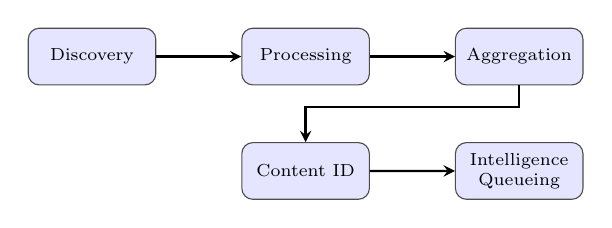
\begin{tikzpicture}[
    scale=0.9,
    transform shape,
    node distance=1.2cm,
    auto,
    phase/.style={rectangle, rounded corners, draw=black!70, fill=blue!10, minimum width=1.8cm, minimum height=0.8cm, align=center, font=\scriptsize},
    arrow/.style={->, >=stealth, thick}
]
    \node[phase] (discovery) {Discovery};
    \node[phase, right=of discovery] (processing) {Processing};
    \node[phase, right=of processing] (aggregation) {Aggregation};
    \node[phase, below=0.8cm of processing] (content) {Content ID};
    \node[phase, right=of content] (intelligence) {Intelligence\\Queueing};

    \draw[arrow] (discovery) -- (processing);
    \draw[arrow] (processing) -- (aggregation);
    \draw[arrow] (aggregation.south) -- ++(0,-0.3) -| (content.north);
    \draw[arrow] (content) -- (intelligence);
\end{tikzpicture}
\caption{The five phases of the Spacedrive indexing pipeline, including intelligence task dispatch.}
\label{fig:indexing_pipeline}
\end{figure}

\begin{itemize}[noitemsep, topsep=0pt]
 \item \textbf{Discovery Phase}: The engine performs a recursive traversal of a \texttt{Location}'s file system. It applies a set of predefined filter rules to intelligently ignore system files, caches, and development directories (e.g., \texttt{.git}, \texttt{node\_modules}). Discovered items are collected into batches for efficient processing.

 \item \textbf{Processing Phase}: Each batch of discovered entries is processed to create or update records in the database. This phase includes \textbf{change detection}, which uses inode tracking and modification timestamps to identify new, modified, or moved files, ensuring that only necessary updates are performed.

 \item \textbf{Aggregation Phase}: For directories, the engine performs a bottom-up traversal to calculate aggregate statistics, such as total size and file counts. This pre-calculation makes directory size lookups an O(1) operation.

 \item \textbf{Content Identification Phase}: For files, this phase generates a content hash (CAS ID---Content-Addressed Storage Identifier) for deduplication. It employs an adaptive hashing strategy: small files are fully hashed, while large files are sampled to maintain performance. This phase also performs file type detection using a combination of extension matching and magic byte analysis.

 \item \textbf{Intelligence Queueing Phase}: After a file's content and type are identified, this new phase dispatches specialized, asynchronous jobs for deeper analysis. For example, an Entry identified as an image may trigger an \texttt{OcrJob} and an \texttt{ImageAnalysisJob}. These intelligence jobs run in the background, populating the Virtual Sidecar System without blocking core indexing.
\end{itemize}

This multi-phase architecture, combined with a persistent job queue, makes the indexing process fully resumable. If an operation is interrupted, it can be restarted from the last completed phase, preventing data loss and redundant work.

\subsubsection{Flexible Indexing Scopes and Persistence}
\label{sec:indexing-scopes}

A key innovation of the Spacedrive indexer is its ability to adapt to different use cases through flexible scopes and persistence modes.

\begin{itemize}[noitemsep, topsep=0pt]
 \item \textbf{Recursive vs. Current Scope}: The indexer can perform a full recursive scan of a directory tree or a shallow, single-level scan of only the immediate contents. The latter is integral to Spacedrive's responsive UI navigation through a "lazy refresh" mechanism. When a user browses a directory, the system instantly presents the existing indexed data from its database. Concurrently, it automatically spawns a non-blocking, shallow indexing job as a side effect of the browse operation. This background job quickly validates the presented data against the live filesystem, ensuring the index remains accurate without sacrificing immediate interactivity. This behavior is configurable at the API level and operates as an internal job rather than a user-initiated action.

 \item \textbf{Persistent vs. Ephemeral Mode}: For managed Locations, indexing results are persisted to the Library's database. However, the indexer also supports an ephemeral, in-memory mode for Browse external or temporary paths without polluting the main index. To ensure a responsive user experience when Browse large unmanaged directories, this mode streams results back to the client in real-time. As the indexer's Discovery phase collects entries into batches , each batch is sent immediately through the Job System's progress channel (\texttt{progress\_tx}) as a \texttt{Progress::Structured} message. The UI can then subscribe to these progress updates and render entries as they arrive, rather than waiting for the entire scan to complete.
\end{itemize}

This flexibility is managed through a unified \texttt{IndexerJobConfig}, which allows for fine-grained control over the indexing process for different scenarios, from background library maintenance to real-time UI interactions.

\subsubsection{Locations and Real-Time Monitoring}

A Spacedrive Library is composed of one or more \textbf{Locations}---managed directories that act as the entry points to a user's physical file systems. The \textbf{Location Watcher} service provides a robust, cross-platform, real-time monitoring system that keeps the Spacedrive index perfectly synchronized with the underlying file system.

\textbf{The Location as a Managed Entity}

When a user adds a directory to a Spacedrive Library, it becomes a \texttt{Location}, a managed entity with its own configuration and lifecycle. This allows for granular control over how different parts of the user's dataspace are handled. Each \texttt{Location} has a specific \textbf{Index Mode} (\texttt{Shallow}, \texttt{Content}, or \texttt{Deep}), enabling users to apply different levels of analysis to different types of content (e.g., deep analysis for a photo library, shallow for a downloads folder).

\textbf{The Location Watcher Service}

The watcher service is the core of Spacedrive's real-time capabilities, providing a resilient and efficient file system monitoring solution.

\textbf{Platform-Specific Optimizations}

A key strength of the watcher is its use of platform-native APIs for optimal performance and reliability. This is a non-trivial engineering challenge, as each OS has unique behaviors.

\begin{itemize}[noitemsep, topsep=0pt]
 \item \textbf{macOS (\texttt{FSEvents})}: The system correctly handles the ambiguous rename and move events from \texttt{FSEvents} by tracking file inodes to reliably link old and new paths.

 \item \textbf{Linux (\texttt{inotify})}: The watcher leverages the efficiency of \texttt{inotify} for direct, recursive directory watching and uses cookie-based event correlation to reliably detect move operations.

 \item \textbf{Windows (\texttt{ReadDirectoryChangesW})}: The implementation is designed to handle Windows-specific filesystem quirks, such as delayed file deletions caused by antivirus software or file locking. It does this by maintaining a "pending deletion" state to verify that a file is truly gone before emitting a deletion event.
\end{itemize}

\textbf{Intelligent Event Processing}

The watcher service is more than a simple event forwarder. It includes an intelligent processing pipeline:

\begin{itemize}[noitemsep, topsep=0pt]
 \item \textbf{Noise Filtering}: The watcher filters out irrelevant events from temporary files (\texttt{.tmp}, \texttt{\textasciitilde backup}), system files (\texttt{.DS\_Store}), and editor-specific files (\texttt{.swp}), ensuring that only meaningful changes are processed.

 \item \textbf{Event Debouncing}: To prevent "event storms" during bulk operations (e.g., unzipping an archive), the system debounces file system events, consolidating rapid-fire changes into single, actionable events.

 \item \textbf{Event Bus Integration}: Processed events are published to the core \texttt{EventBus}---a centralized message routing system that enables loose coupling between services---where they trigger other components. For example, an \texttt{EntryModified} event will trigger the indexer to re-analyze a file, the search service to update its index, and the sync service to propagate the change to other devices.
\end{itemize}

This robust, real-time monitoring system is what transforms Spacedrive from a static file index into a dynamic, live dataspace that always reflects the true state of a user's files.

\subsubsection{Offline Recovery and Stale Detection}
\label{sec:offline-recovery}

While the Location Watcher provides real-time monitoring during normal operation, a critical challenge arises when Spacedrive itself is offline---whether due to system shutdown, crashes, or disconnected storage volumes. When the system returns online, it must efficiently detect and reconcile any filesystem changes that occurred during its absence.

\textbf{Offline Window Tracking}

Spacedrive tracks its core uptime and persists the timestamp of its last shutdown. Upon startup, the system calculates the "offline window"---the period between the last shutdown time and the current time. This window defines the temporal scope within which filesystem changes may have occurred undetected. By comparing this offline period against filesystem modification times, the system can efficiently identify which portions of the filesystem require validation.

\textbf{Intelligent Stale Detection}

Rather than performing expensive full filesystem scans after every offline period, Spacedrive leverages a key property of modern filesystems: modification time propagation. On most operating systems (Windows NTFS, macOS APFS, and Linux ext4/btrfs), changes to files within nested directories update the modification timestamps of parent directories up the tree.

The stale detection algorithm operates as follows:
\begin{enumerate}[noitemsep, topsep=0pt]
\item Walk the directory tree starting from each Location root
\item Compare directory modification times against the offline window
\item If a directory's modification time falls within the offline window, mark it for deep scanning
\item Recursively scan only marked directories and their contents
\item Update the index with discovered changes while preserving unchanged portions
\end{enumerate}

This approach dramatically reduces the re-indexing overhead. For example, in a Location with 100,000 files across 10,000 directories where only 50 files changed during offline time, the system might only need to deeply scan 200-300 directories rather than the entire tree.

\textbf{Graceful Degradation for Unsupported Filesystems}

For filesystems that don't reliably propagate modification times (such as certain network filesystems or FAT32), Spacedrive detects this limitation and falls back to an ephemeral deep indexing strategy. This approach leverages the existing multi-phase indexing pipeline but constrains execution to only the Discovery phase---rapidly traversing the filesystem to create lightweight Entry records without performing expensive content analysis. By comparing these ephemeral entries against the persisted database state, the system can efficiently identify additions, deletions, and modifications based on file metadata. Only the detected changes are then queued for full processing through the remaining indexing phases (content identification, media analysis, etc.). The system maintains filesystem capability profiles to automatically select the optimal detection strategy per Location.

This hybrid approach ensures Spacedrive maintains its performance advantages while guaranteeing index integrity, addressing a fundamental limitation of purely real-time monitoring systems.

% --- SECTION 4.4: THE TRANSACTIONAL ACTION SYSTEM ---
\subsection{The Transactional Action System}
\label{sec:action-system}

\begin{keytakeaways}
\begin{itemize}[noitemsep, topsep=0pt]
\item \textbf{Revolutionary Paradigm}: Preview any operation before execution - see exactly what will happen
\item \textbf{Guaranteed Completion}: Operations become durable jobs that complete even across device disconnections
\item \textbf{Centralized Control}: All operations flow through type-safe action system with full audit logging
\end{itemize}
\end{keytakeaways}

Traditional file management is immediate and often unforgiving. Operations execute instantly, with no opportunity to preview the outcome, leading to uncertainty, especially in complex tasks like cross-device backups or data reorganization. Spacedrive introduces a paradigm shift with its \textbf{Transactional Action System with Pre-visualization}, which treats user intent as a transactional, verifiable operation.

This system allows any file system operation to be simulated in a "dry run" mode before execution. Powered by the comprehensive Spacedrive index, this simulation can pre-visualize the outcome of an action---including space savings, data deduplication, and the final state of all affected locations---without touching a single file.

\subsubsection{The Action Lifecycle: Preview, Commit, Verify}

Every action in Spacedrive follows a transactional lifecycle:

\textbf{Intent \& Preview}: The user expresses an intent (e.g., "move photos from my phone to my NAS"). Spacedrive uses its index to generate a preview of the outcome. The system can accurately forecast the end state because it has a complete metadata map of all user data.

\textbf{Commit}: Once the user approves the preview, the action is committed to the Durable Job System. It becomes a resilient, resumable job that is guaranteed to execute, even if devices are offline or network connectivity is interrupted.

\textbf{Execution \& Verification}: The job is executed by the appropriate device agents when they come online. The system continuously works to complete the job, verifying each step against the initial plan. This durability ensures that user intent is always fulfilled without data loss or corruption.

\begin{figure}[ht!]
\centering
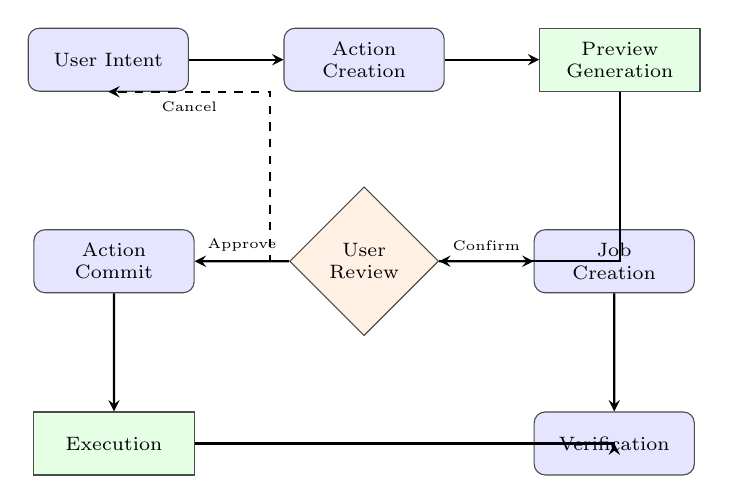
\begin{tikzpicture}[
    scale=0.8,
    node distance=1.5cm and 1.2cm,
    auto,
    state/.style={rectangle, rounded corners, draw=black!70, fill=blue!10, text width=1.8cm, minimum height=0.8cm, align=center, font=\scriptsize},
    decision/.style={diamond, draw=black!70, fill=orange!10, text width=1.3cm, minimum height=0.8cm, align=center, font=\scriptsize, inner sep=1pt},
    process/.style={rectangle, draw=black!70, fill=green!10, text width=1.8cm, minimum height=0.8cm, align=center, font=\scriptsize},
    arrow/.style={->, >=stealth, thick},
    label/.style={font=\tiny, align=center}
]
    % Top row
    \node[state] (intent) {User Intent};
    \node[state, right=of intent] (action) {Action\\Creation};
    \node[process, right=of action] (preview) {Preview\\Generation};

    % Bottom row
    \node[decision, below=1.2cm of action] (review) {User\\Review};
    \node[state, left=of review] (commit) {Action\\Commit};
    \node[state, right=of review] (job) {Job\\Creation};

    % Execution nodes
    \node[process, below=of commit] (execute) {Execution};
    \node[state, below=of job] (verify) {Verification};

    % Arrows
    \draw[arrow] (intent) -- (action);
    \draw[arrow] (action) -- (preview);
    \draw[arrow] (preview) |- (review);
    \draw[arrow] (review) -- node[label, above] {\tiny Approve} (commit);
    \draw[arrow] (review) -- node[label, above] {\tiny Confirm} (job);
    \draw[arrow] (commit) -- (execute);
    \draw[arrow] (job) -- (verify);
    \draw[arrow] (execute) -| (verify);

    % Cancel path
    \draw[arrow, dashed] (review.west) -- ++(-0.3,0) |- node[label, near end] {\tiny Cancel} (intent.south);
\end{tikzpicture}
\caption{The Action Lifecycle: From user intent through preview, approval, and execution}
\label{fig:action-lifecycle}
\end{figure}

\begin{figure}[ht!]
\centering
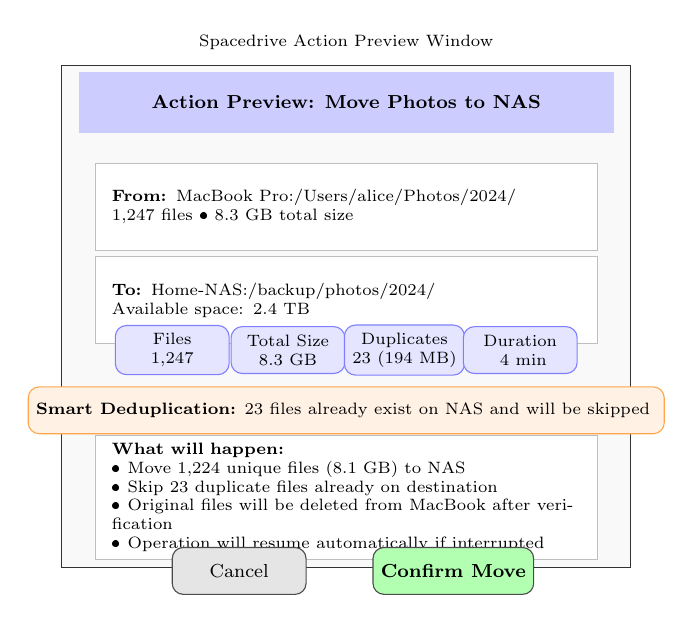
\begin{tikzpicture}[
    scale=0.85,
    transform shape,
    % UI Frame
    uiframe/.style={rectangle, draw=black!80, fill=gray!5, minimum width=8.5cm, minimum height=7.5cm},
    % UI Elements
    header/.style={rectangle, fill=blue!20, minimum width=8cm, minimum height=0.9cm, align=center, font=\footnotesize\bfseries},
    section/.style={rectangle, draw=gray!50, fill=white, minimum width=7.5cm, minimum height=1.3cm, align=left, font=\scriptsize},
    button/.style={rectangle, rounded corners, draw=black!70, minimum width=2cm, minimum height=0.7cm, align=center, font=\footnotesize},
    cancelbutton/.style={button, fill=gray!20},
    confirmbutton/.style={button, fill=green!30},
    stat/.style={rectangle, rounded corners, draw=blue!50, fill=blue!10, minimum width=1.7cm, minimum height=0.7cm, align=center, font=\scriptsize},
    warningbox/.style={rectangle, rounded corners, draw=orange!70, fill=orange!10, minimum width=7.5cm, minimum height=0.7cm, align=center, font=\scriptsize}
]
    % Main Frame
    \node[uiframe] (frame) {};

    % Header
    \node[header] at (0, 3.2) {Action Preview: Move Photos to NAS};

    % Source Section
    \node[section, anchor=north, text width=7cm] at (0, 2.3) (source) {
        \textbf{From:} MacBook Pro:/Users/alice/Photos/2024/\\
        \scriptsize 1,247 files • 8.3 GB total size
    };

    % Destination Section
    \node[section, anchor=north, text width=7cm] at (0, 0.9) (dest) {
        \textbf{To:} Home-NAS:/backup/photos/2024/\\
        \scriptsize Available space: 2.4 TB
    };

    % Statistics Row
    \node[stat] at (-2.6, -0.5) {Files\\1,247};
    \node[stat] at (-0.87, -0.5) {Total Size\\8.3 GB};
    \node[stat] at (0.87, -0.5) {Duplicates\\23 (194 MB)};
    \node[stat] at (2.6, -0.5) {Duration\\~4 min};

    % Deduplication Notice
    \node[warningbox] at (0, -1.4) {
        \textbf{Smart Deduplication:} 23 files already exist on NAS and will be skipped
    };

    % Preview Details
    \node[section, minimum height=1.7cm, text width=7cm] at (0, -2.7) {
        \textbf{What will happen:}\\
        \scriptsize
        • Move 1,224 unique files (8.1 GB) to NAS\\
        • Skip 23 duplicate files already on destination\\
        • Original files will be deleted from MacBook after verification\\
        • Operation will resume automatically if interrupted
    };

    % Buttons
    \node[cancelbutton] at (-1.6, -3.8) {Cancel};
    \node[confirmbutton] at (1.6, -3.8) {\textbf{Confirm Move}};

    % Title
    \node[font=\scriptsize, above=0.1cm of frame.north] {Spacedrive Action Preview Window};
\end{tikzpicture}
\caption{Action Preview UI Mockup: Users see exactly what will happen before any files are modified, including deduplication savings and potential issues.}
\label{fig:action-preview-ui}
\end{figure}

\subsubsection{The Simulation Engine}

The Spacedrive index serves as a powerful simulation engine. Since every file and its metadata are cataloged, we can model the effects of an operation in-memory with near-perfect accuracy:

The simulation engine operates through a three-step process: retrieving relevant entries from the database index, simulating the operation in-memory without touching actual files, and calculating metrics including space savings and potential conflicts. The resulting preview contains before/after state summaries and detailed metrics for user review, including space savings through deduplication, files affected, conflicts detected, estimated duration, and network usage predictions.

\textbf{Operational Conflict Detection}

The simulation engine proactively identifies operational conflicts that would cause traditional file operations to fail:
\begin{itemize}[noitemsep, topsep=0pt]
\item \textbf{Storage Constraints}: Calculates exact space requirements and verifies availability on target devices
\item \textbf{Permission Violations}: Detects write-protected locations or access-restricted files before attempting operations
\item \textbf{Path Conflicts}: Identifies naming collisions and circular reference issues in complex move operations
\item \textbf{Resource Limitations}: Estimates memory and bandwidth requirements against device capabilities
\end{itemize}

This comprehensive conflict detection represents Spacedrive's primary defense for data integrity. The simulation engine prevents operational conflicts entirely by catching them during the planning phase, while synchronization conflicts from concurrent modifications across devices are handled through intelligent domain-specific merging strategies (detailed in Section 15). This dual approach ensures exceptional reliability in distributed file management.

This is particularly powerful when combined with Native Storage Tiering (Section~\ref{sec:volume-foundation}). If a user attempts an operation on a Location they have marked with a \texttt{Hot} logical class, but it resides on a Volume physically classified as \texttt{Cold}, the simulation engine generates a clear warning in the preview: "⚠️ This operation targets a 'hot' location on a slow archive drive. Estimated completion time may be longer than expected." This prevents user frustration by aligning expectations with physical reality before any action is committed.

\paragraph{Intelligent Time Estimation}
The Simulation Engine combines multiple data sources to provide accurate operation time estimates:

\begin{itemize}
    \item \textbf{Volume Performance Metrics}: Real-time read/write speeds from continuous monitoring
    \item \textbf{Network Conditions}: Current bandwidth and latency from Iroh's measurements
    \item \textbf{Historical Data}: Previous operations on similar files and paths
    \item \textbf{Operation Complexity}: Number of files, total size, and fragmentation
    \item \textbf{Storage Type Awareness}: Different strategies for local vs cloud storage
\end{itemize}

For example, when copying 10GB across devices, the estimation considers:
\begin{itemize}
    \item Source volume read speed: 250 MB/s (measured)
    \item Network throughput: 45 MB/s (current P2P bandwidth)
    \item Destination write speed: 180 MB/s (measured)
    \item Bottleneck: Network at 45 MB/s
    \item Estimated time: 3 minutes 45 seconds (with 10\% buffer)
\end{itemize}

For cloud operations, additional factors apply:
\begin{itemize}
    \item API rate limits (e.g., 1000 requests/second for S3)
    \item Chunk size optimization (balancing throughput vs memory)
    \item Parallel stream count (typically 4-8 for cloud providers)
    \item Resume capability for long-running transfers
\end{itemize}

This transparency helps users make informed decisions about when and how to execute operations, especially for large-scale cloud migrations.

\subsubsection{Centralized Operation Control}

Rather than allowing direct operation dispatch throughout the codebase, Spacedrive routes all user actions through a centralized \textbf{Action System} that provides consistent validation, execution, and logging:

The Action System employs a centralized enumeration that captures every possible user operation, distinguishing between global actions (system-level operations like library creation) and library-scoped actions (operations within a specific Library context). This design provides clear authorization boundaries and enables comprehensive tracking of all user-initiated operations.

\subsubsection{Type-Safe Action Construction}

The system employs a \textbf{builder pattern} for type-safe action construction that integrates seamlessly with CLI and API inputs:

\begin{lstlisting}[language=Rust, caption={Type-safe action construction with builder pattern}]
// Builder pattern ensures valid action construction
let action = FileCopyAction::builder()
    .source_paths(vec!["/docs/report.pdf", "/docs/data.csv"])
    .target_path("/backup/2024/")
    .mode(TransferMode::Move)  // Move instead of copy
    .verify_checksum(true)      // Ensure integrity
    .preserve_timestamps(true)   // Keep original dates
    .on_conflict(ConflictStrategy::Skip)
    .build()?;  // Returns error if invalid combination

// Actions are serializable for durability
let job = Job::from_action(action);
queue.push(job).await?;
\end{lstlisting}

This builder approach provides \textbf{compile-time validation} of action parameters, preventing invalid operations from reaching the execution layer while maintaining ergonomic APIs for both programmatic and command-line usage.

\subsubsection{Comprehensive Audit Logging}

Every library-scoped action automatically receives comprehensive audit logging through the database layer:

\begin{table}[h]
\footnotesize
\centering
\begin{tabular}{@{}ll@{}}
\toprule
\textbf{Audit Field} & \textbf{Information Captured} \\
\midrule
Action Type & Operation performed (e.g., "file.copy") \\
Device & Initiating device identifier \\
Resources & Files/folders/locations affected \\
Status & Previewed → Committed → Complete \\
Job Link & Background job reference \\
Timing & Start/end times, duration \\
Errors & Failure details if applicable \\
Results & Outcome and metrics \\
\bottomrule
\end{tabular}
\caption{Comprehensive audit trail fields}
\label{tab:audit-fields}
\end{table}

The \textbf{ActionManager} automatically creates audit entries for both preview and execution phases, tracking the complete action lifecycle from initial intent through final completion.

\subsubsection{Dynamic Handler Registry}

The Action System employs a dynamic registry pattern using Rust's \textbf{inventory} crate for automatic handler discovery:

\textbf{Extensible Action Handler System}

Spacedrive's Action System uses a self-registering architecture that automatically discovers available operations:

\begin{itemize}[noitemsep, topsep=0pt]
 \item \textbf{Automatic Discovery}: New operations register themselves when added to the codebase
 \item \textbf{No Central Maintenance}: Adding new file operations requires no manual registry updates
 \item \textbf{Type Safety}: Each operation handler is validated at compile time
 \item \textbf{Consistent Interface}: All operations (file copy, location management, etc.) follow the same patterns
\end{itemize}

This architecture enables easy extension of Spacedrive's capabilities while maintaining system reliability and consistent user experience across all operations.

\subsubsection{Foundation for Advanced Capabilities}

The Action System's centralized architecture enables sophisticated features that would be difficult to implement across a distributed codebase:

\textbf{\plannedSection{Enterprise-Grade RBAC Foundation}}

The centralized Action System is architected as the foundation for comprehensive Role-Based Access Control (RBAC), essential for team collaboration and enterprise deployment:

\begin{itemize}[noitemsep, topsep=0pt]
 \item \textbf{Role Definitions}: Standard roles like "Viewer" (read-only), "Contributor" (read/write), "Manager" (full control), and custom roles tailored to organizational needs
 \item \textbf{Granular Permissions}: Action-level control enabling scenarios like "can upload but not delete" or "can tag but not move files"
 \item \textbf{Location-Based Access}: Restrict access to specific Locations or paths (e.g., "Finance team accesses /financial-data, Creative team accesses /assets")
 \item \textbf{Inheritance and Groups}: Permission inheritance through organizational groups with override capabilities
 \item \textbf{Temporal Controls}: Time-based access for contractors or temporary project members
 \item \textbf{Audit Trail Integration}: Every permission check logged with full context for compliance and security reviews
\end{itemize}

\textbf{\plannedSection{Intelligent Undo Capabilities}}

The comprehensive audit trail provides the foundation for sophisticated operation reversal:

\begin{itemize}[noitemsep, topsep=0pt]
 \item \textbf{Safe Undo Logic}: System understands how to safely reverse each operation type
 \item \textbf{Dependency Tracking}: Prevents undoing operations that other actions depend on
 \item \textbf{Selective Reversal}: Undo specific parts of complex operations (e.g., "undo copying just these 3 files")
 \item \textbf{Cross-Device Coordination}: Undo operations that span multiple devices with proper cleanup
\end{itemize}

\subsubsection{Remote Action Dispatch}

A key benefit of combining the Action System with the \texttt{SdPath} universal addressing scheme is the ability to dispatch actions where the execution occurs transparently on a remote device. For example, a \texttt{FileCopyAction} can specify a source \texttt{SdPath} on Device A and a destination \texttt{SdPath} on Device B. When this action is committed, the Job System intelligently routes the work. It creates a sender job on Device A and a corresponding receiver job on Device B, which coordinate the transfer over the secure P2P network. This architecture makes complex cross-device workflows trivial to express and execute, as the underlying network communication and state management are handled automatically by the core engine. All remote operations are still subject to the same validation, preview, and audit logging as local actions, ensuring a consistent security model across the entire VDFS.

\subsubsection{Handling File Ingestion and Uploads}
\label{sec:ingestion-workflow}
While much of Spacedrive's power comes from indexing existing files, a critical function is the ingestion of new files from external sources, such as a web interface or a drag-and-drop operation into the application. This process is managed through a specialized \textbf{Ingestion Workflow}, built upon the Transactional Action System.

At the heart of this workflow is the concept of a user-configurable \textbf{Ingest Location}, colloquially known as an "Inbox" or "quarantine zone." This is a designated default directory on a preferred, often always-online, device (such as a home server or a Cloud Core instance). When a user uploads a file without specifying an explicit destination:

\begin{enumerate}[noitemsep, topsep=0pt]
    \item A \texttt{FileIngestAction} is created. The source is the uploaded data stream, and the destination defaults to the primary Ingest Location.
    \item The Action System routes this job to the destination device, which handles the secure file transfer via the Iroh protocol.
    \item Upon successful transfer, the file is written to the Ingest Location, and a new \texttt{Entry} is created in the VDFS index.
\end{enumerate}

This architecture ensures that new files are added to the user's dataspace in a transactional, reliable manner. Once the file becomes a managed \texttt{Entry}, it is immediately available for the AI layer to analyze and organize, as detailed in Section~\ref{sec:ai-native-ingestion}.

% --- SECTION 4.5: LIBRARY SYNC & NETWORKING ---
\subsection{Library Sync and Networking}
\label{sec:sync-networking}

\begin{keytakeaways}
\begin{itemize}[noitemsep, topsep=0pt]
\item \textbf{Domain Separation}: Avoids CRDT complexity by separating index, metadata, and file operations
\item \textbf{Unified Networking}: Single Iroh endpoint handles all protocols with 90\%+ NAT traversal
\item \textbf{Intelligent Sync}: VDFS index enables instant change detection and global deduplication
\end{itemize}
\end{keytakeaways}

Spacedrive's distributed architecture requires sophisticated synchronization and networking capabilities to maintain consistency across devices while preserving the local-first philosophy. This section presents the unified approach to synchronization through domain separation and the Iroh-powered networking infrastructure that enables reliable peer-to-peer communication.

\subsubsection{Library Sync via Domain Separation}
\label{sec:library-sync}

Traditional distributed consensus algorithms struggle with the mixed requirements of personal data management. Spacedrive's \textbf{Library Sync} architecture tames this complexity by separating synchronization into three distinct domains, each with tailored conflict resolution strategies:

\textbf{Index Sync (Filesystem State)}

Each device maintains authoritative control over its own filesystem index. Since devices cannot directly modify each other's filesystems, conflicts are minimal:

\begin{itemize}[noitemsep, topsep=0pt]
 \item \textbf{Data}: Entry records, device-specific paths, Location metadata
 \item \textbf{Conflicts}: Extremely rare---only occur when multiple devices simultaneously scan the same shared storage
 \item \textbf{Resolution}: Device authority model---each device controls its own filesystem state completely
\end{itemize}

\textbf{User Metadata Sync (Content Tags and Ratings)}

Content-universal metadata that should follow files across devices uses union-merge strategies:

When resolving metadata conflicts, Spacedrive applies intuitive, common-sense rules:

\begin{itemize}[noitemsep, topsep=0pt]
 \item \textbf{Tags}: Automatically merge all tags---if you label a photo "family" on one device and "vacation" on another, the result is "family, vacation"
 \item \textbf{Favorites}: Use OR logic---if either device marks something as favorite, it stays favorite
 \item \textbf{Ratings}: Most recent rating wins, with clear notification to the user
 \item \textbf{Notes}: Combine with timestamps so users can review and edit the merged content
\end{itemize}

\textbf{File Operations (Explicit Transfer)}

Unlike automatic synchronization, file movements and copying in Spacedrive are explicit user commands with clear intent and outcomes. When a user requests "copy my photos to the backup drive," this creates a deliberate operation with:

\begin{itemize}[noitemsep, topsep=0pt]
 \item Clear source and destination specifications
 \item Predictable error handling and retry logic
 \item Progress tracking and user notification
 \item Automatic filesystem change detection that updates the index
\end{itemize}

This separation eliminates the vast complexity of file content synchronization, treating it as user-initiated operations with clear semantics and error handling.

\subsubsection{Iroh-Powered Network Infrastructure}

Spacedrive's networking architecture represents a fundamental shift from fragmented, protocol-specific implementations to a \textbf{unified networking layer} powered by Iroh. This consolidation eliminates the complexity of managing separate networking stacks for sync, file transfer, and device discovery, achieving enterprise-level connectivity reliability on consumer networks:

\textbf{Superior NAT Traversal}

The networking service employs a unified architecture where all protocols share a single Iroh endpoint. Through Application-Layer Protocol Negotiation (ALPN), different features like pairing, file transfer, and sync seamlessly multiplex over the same connections. This eliminates the need for separate networking implementations per feature---a single connection between devices supports all protocols concurrently, with automatic stream management and shared session encryption.

Performance improvements over the previous fragmented implementation:
\begin{itemize}[noitemsep, topsep=0pt]
 \item \textbf{90\%+ NAT traversal success} (versus 70\% with libp2p)
 \item \textbf{Sub-2-second connection establishment} (down from 3-5 seconds)
 \item \textbf{60\% reduction in networking code} through protocol consolidation
 \item \textbf{Single connection per device pair} supporting all protocols concurrently
 \item \textbf{Native mobile platform support} (iOS, Android, ESP32)
\end{itemize}

\textbf{QUIC-Based Transport Layer}

Iroh's built-in QUIC transport provides integrated transport features including ChaCha20-Poly1305 encryption, stream multiplexing for concurrent operations, BBR congestion control for optimal bandwidth utilization, and zero round-trip connection resumption for seamless reconnection.

\textbf{Automatic Network Discovery and Connection}

Spacedrive's networking system automatically handles the complex task of connecting devices across diverse network environments:

\begin{itemize}[noitemsep, topsep=0pt]
 \item \textbf{Multi-Path Discovery}: Devices find each other through multiple channels simultaneously---local network broadcasting, DNS-based discovery, and relay server coordination.
 \item \textbf{Intelligent Relay Routing}: When direct connection isn't possible (due to firewalls or NAT), the system automatically routes through secure relay servers while maintaining end-to-end encryption.
 \item \textbf{Zero-Configuration Setup}: Users simply pair devices once---the networking layer handles all future connection establishment, routing decisions, and failover scenarios transparently.
\end{itemize}

\paragraph{Self-Hosted Relay Infrastructure}
While Spacedrive provides public relay servers for convenience, the architecture fully supports self-hosted deployments:

\begin{itemize}
    \item \textbf{Zero-Trust Option}: Organizations can run private relay networks
    \item \textbf{Simple Deployment}: Single binary with minimal configuration
    \item \textbf{Geographic Distribution}: Deploy relays near users for optimal performance
    \item \textbf{Compliance Ready}: Keep all traffic within organizational boundaries
\end{itemize}

This flexibility makes Spacedrive suitable for:
\begin{itemize}
    \item Enterprises requiring complete data sovereignty
    \item Regions with data residency requirements
    \item Air-gapped networks with no external connectivity
    \item Organizations building private overlay networks (similar to Tailscale)
\end{itemize}

The relay service can be deployed as a standalone component, in Kubernetes, or as a managed service, providing deployment flexibility to match any infrastructure requirement.

\paragraph{Network Architecture Flexibility}
The Iroh-based networking supports multiple topologies:

\begin{verbatim}
Public Cloud (Default):
Device A ←→ Public Relay ←→ Device B
         ↘              ↙
          Direct (if possible)

Self-Hosted:
Device A ←→ Private Relay ←→ Device B
         ↘               ↙
          Direct (always preferred)

Hybrid:
Corporate ←→ Private Relay ←→ Public Relay ←→ Personal
Devices                                        Devices
\end{verbatim}

This flexibility ensures Spacedrive can adapt to any network environment while maintaining its peer-to-peer principles.

\subsubsection{Spacedrop: Ephemeral Secure Sharing}

Beyond trusted device pairing, Spacedrive implements \textbf{Spacedrop}---an ephemeral file sharing protocol that enables secure transfers between any devices without prior relationships. Built on the same Iroh infrastructure but with distinct security properties:

\textbf{Perfect Forward Secrecy}: Each Spacedrop session uses ephemeral ECDH key exchange, ensuring that compromising device keys cannot decrypt past transfers. The protocol generates fresh ephemeral keys for each transfer session, which are immediately discarded after completion.

\textbf{User Consent Model}: Unlike automatic transfers between paired devices, every Spacedrop requires explicit receiver acceptance, maintaining user control over incoming data. The receiver sees the sender's device name, file metadata, and optional message before accepting.

\textbf{Multi-Modal Discovery}: Spacedrop employs a sophisticated discovery mechanism that adapts to available connectivity:
\begin{itemize}[noitemsep, topsep=0pt]
    \item \textbf{Local Network}: mDNS broadcasts for same-network discovery
    \item \textbf{Bluetooth Low Energy}: Optional BLE advertisements for true proximity detection, enabling discovery even without shared Wi-Fi
    \item \textbf{DHT Fallback}: Internet-wide discovery using Iroh's distributed hash table when local discovery fails
\end{itemize}

\textbf{Relay Extension}: Spacedrop can optionally leverage relay nodes (either self-hosted or through Spacedrive Cloud) to enable asynchronous transfers. Users can "drop" files to a relay and receive a shareable link, allowing recipients to download later---combining the security of Spacedrop with the convenience of services like WeTransfer.

\subsubsection{Intelligent File Synchronization}

While Spacedrive's primary function is to create a unified virtual index, this comprehensive "world model" serves as a powerful foundation for advanced physical file synchronization. Unlike traditional stateless data-moving utilities that must re-evaluate source and destination on every run, Spacedrive leverages its persistent, real-time VDFS index to perform intelligent, efficient, and reliable file synchronization.

\textbf{VDFS-Powered Sync Operations}

At its core, all synchronization operations are managed by the \textbf{Transactional Action System}, ensuring they benefit from the same pre-visualization, durability, and conflict prevention mechanisms as other file operations. The key advantage lies in how Spacedrive prepares for a sync:

\begin{itemize}[noitemsep, topsep=0pt]
    \item \textbf{Instant Change Detection}: The Location Watcher service ensures the VDFS index is always current. When a sync is initiated, the system already knows the precise delta without needing to perform a full scan.
    \item \textbf{Global Context and Deduplication}: The index has a global view of all content across all devices. Before transferring a file, Spacedrive checks its \textbf{Content ID} to avoid redundant transfers.
    \item \textbf{Optimal Path Resolution}: Leveraging the \texttt{SdPath} universal addressing system, Spacedrive can find the most efficient source for a piece of content.
\end{itemize}

\textbf{Synchronization Modes}

The Spacedrive architecture supports multiple synchronization policies, managed as durable relationships between Locations:

\begin{itemize}[noitemsep, topsep=0pt]
    \item \textbf{Replicate (One-Way Sync)}: A target Location is made to be an exact replica of a source Location. The simulation engine calculates the delta by comparing index states and provides a clear preview before any changes are committed.
    \item \textbf{Two-Way Sync}: Spacedrive establishes a persistent \texttt{SyncRelationship} between two Locations with real-time monitoring. When changes are detected, corresponding sync actions are automatically generated based on user-defined policies.
\end{itemize}

This stateful, always-on monitoring eliminates the need for periodic manual syncs. In the event of conflicts, Spacedrive's metadata conflict resolution strategies are invoked to merge changes intelligently or prompt the user for a decision.

% --- SECTION 4.6: THE AI LAYER ---
\subsection{AI-Native VDFS: From Semantic Search to Intelligent Management}
\label{sec:ai-native}

\begin{keytakeaways}
\begin{itemize}[noitemsep, topsep=0pt]
\item \textbf{AI-Native Design}: Your file index becomes a comprehensive "world model" that AI agents can understand and reason about
\item \textbf{Natural Language}: Say "organize my tax documents" and watch as the AI converts your intent into safe, previewable actions
\item \textbf{Privacy-First AI}: Run models locally with Ollama for complete privacy, or use cloud AI with transparent controls
\end{itemize}
\end{keytakeaways}

While many systems treat AI as an additive feature, Spacedrive is architected as an \textbf{AI-native dataspace}. The comprehensive, always-current index of the user's files serves as a perfect "world model" for an AI agent to reason about. This enables a shift from reactive file management (issuing manual commands) to a proactive, collaborative model where both the user and an AI agent can manage the dataspace, with the human always in the loop. This vision builds upon decades of research in semantic file systems~\cite{gifford_sfs_1991}, information retrieval~\cite{dumais_stuff_2003}, and ubiquitous computing~\cite{weiser_ubiquitous_1991}.

This is achieved through a flexible, privacy-first architecture that is model-agnostic, supporting both powerful cloud services and local models running on user hardware via interfaces like Ollama.

\subsubsection{A Day in Alice's Digital Life}

To illustrate how these capabilities transform everyday file management, consider Alice, a freelance designer juggling multiple projects across various devices and storage locations.

\textit{Monday morning}: Alice sits down at her desk and asks Spacedrive: ``Find my design assets from last fall that I never exported.'' Behind this simple request, a sophisticated dance begins:

\textbf{The AI Observes}: Spacedrive's indexing system has already performed deep analysis on Alice's files. It knows that her Sketch and Figma files from September through November contain layer names like ``v3-final'' and ``client-approved,'' but lack corresponding PNG or PDF exports in nearby folders. The system has extracted color palettes, identified design patterns, and even transcribed text from her design review recordings.

\textbf{The AI Orients}: Cross-referencing the temporal query ``last fall'' with file metadata, the AI identifies 47 design files. It notices from Alice's audit log that she typically exports finals to a ``Deliverables'' folder, but these particular projects show no such exports. The AI also detects that several files have ``URGENT'' in their layer names---a pattern it has learned indicates deadline pressure that might have caused Alice to skip her usual export workflow.

\textbf{The AI Decides}: Rather than simply listing files, the AI formulates a helpful action plan. It generates a structured proposal: ``I found 47 design files from last fall without exports. 12 appear to be final versions based on your naming patterns. Would you like me to batch export these as PNGs to your usual Deliverables folder?''

Alice reviews the proposed \texttt{BatchExportAction}, which shows exactly which files will be processed and where the exports will be saved. With one click, she approves, and the operation joins the durable job queue.

\textit{Later that week}: The AI notices Alice has been manually moving screenshot files from her Desktop to project folders every few days. Having observed this pattern through the audit log, it proactively suggests: ``I've noticed you regularly organize screenshots into project folders. I can automatically move new screenshots to the relevant project based on the window title captured in the metadata. Would you like me to set this up?''

This isn't just automation---it's intelligent assistance that learns and adapts while keeping Alice in complete control.

\subsubsection{The Agentic Loop: Observe, Orient, Act}

Spacedrive's AI capabilities are built on a classic agentic loop, where each stage is powered by a core component of the VDFS architecture:

\textbf{Observe}: The Indexing System is the sensory input. During the \textbf{deep indexing phase}, it goes beyond basic metadata to perform AI-powered analysis, extracting rich context like image content, video transcripts, and document summaries. This enriches the Spacedrive index, providing the AI with a deep understanding of the user's data.

\textbf{Orient}: With a complete "world model" in its index, the AI can orient itself. It analyzes file content, user-applied metadata (tags, ratings), and historical user actions (from the audit\_log table) to understand context, identify patterns, and recognize organizational inconsistencies.

\textbf{Decide \& Act}: The AI formulates a plan and proposes it as a structured Action. This is a critical safety and control mechanism; the AI does not execute arbitrary commands but is constrained to the same safe, verifiable primitives available to the user. A user command like "Archive my old projects from last year that are over 1GB" is translated directly into a FileCopyAction.

\subsubsection{Natural Language Management}

The Action System serves as a stable, well-defined API that can be used to fine-tune language models. This allows Spacedrive to translate complex user requests from natural language into a series of verifiable actions.

As we saw with Alice's request to ``find design assets from last fall that I never exported,'' the system seamlessly translates natural language into precise operations. Similarly, a command like ``Move my last 3 screen recordings from the desktop to the 'Clips' folder on my NAS'' is processed through semantic search to identify the relevant files, then translated into a structured \texttt{FileCopyAction} with appropriate source paths, destination, and move semantics.

The generated action is processed through the Action System (Section~\ref{sec:action-system}), providing a preview before execution. This keeps the human in the loop, with AI serving as an interpreter rather than an opaque automaton.

\subsubsection{Proactive Assistance and Optimization}

Beyond executing commands, the AI agent can proactively identify opportunities to help the user. By observing patterns, it can suggest helpful actions.

\textbf{Organizational Suggestions}: As demonstrated in Alice's workflow, when the AI observed her repeatedly moving screenshots from the Desktop to project folders, it proactively offered to automate this pattern. The architecture enables such capabilities---if the indexer identifies a screen recording on the Desktop and the agent observes from historical actions that the user consistently moves such files to a \texttt{\textasciitilde/Videos/Screen Recordings} folder, it could generate a suggested \texttt{FileCopyAction} for the user to approve with a single click.

\textbf{Deduplication Opportunities}: The agent can periodically scan for duplicated content across devices and suggest a "cleanup" action that consolidates files and frees up space, presenting a clear preview of the space savings.

\textbf{Data Guardian Mode}: Most importantly, the AI acts as a proactive data guardian by leveraging the redundancy intelligence provided by the Content Identity system (detailed in Section~\ref{sec:content-identity}). When Alice imports her daughter's graduation photos—irreplaceable memories captured in a single afternoon—the AI immediately recognizes these as new, unique files existing only on her laptop through the Content Identity's redundancy tracking. Understanding the importance of such content (through semantic analysis of filenames like "Emma\_Graduation\_2024"), it generates a critical suggestion: "I noticed you've added 523 graduation photos that currently exist only on your MacBook. These precious memories could be lost if your laptop fails. Would you like me to create backups on your Home NAS and Cloud Storage?" The suggestion appears as a pre-visualized Action showing exactly which files will be copied and where, giving Alice confidence to protect her memories with a single click.

The AI system analyzes user behavior patterns from the \texttt{audit\_log} table to identify organizational preferences, then suggests actions when files violate established patterns. Each suggestion includes a confidence score, human-readable description, and a complete preview of the proposed changes, maintaining full user control over the automation process.

\paragraph{Intelligent Ingestion Sorting}
\label{sec:ai-native-ingestion}
The AI agent's proactive capabilities are particularly powerful when applied to the file ingestion workflow (Section~\ref{sec:ingestion-workflow}). When new files arrive in the user's designated Ingest Location, the AI's agentic loop is triggered:
\begin{itemize}[noitemsep, topsep=0pt]
    \item \textbf{Observe}: The AI detects new \texttt{Entry} records in the Ingest Location.
    \item \textbf{Orient}: It performs content analysis on the new files (e.g., identifying a PDF as a receipt, a PNG as a screenshot of a specific application) and cross-references this with the user's historical organization patterns from the \texttt{audit\_log} table. For instance, it may notice that PDFs with the word "Invoice" are consistently moved to a "\texttt{/Finances/Invoices}" directory.
    \item \textbf{Decide \& Act}: Based on this analysis, the AI formulates and proposes a \texttt{FileCopyAction} or \texttt{FileMoveAction} to the user. The user is presented with a clear suggestion: "I noticed a new invoice landed in your Inbox. Would you like me to move it to your 'Invoices' folder?". This suggestion is a standard, pre-visualized Action that the user can approve with a single click, ensuring human-in-the-loop control over all automated organization.
\end{itemize}

\subsubsection{File Intelligence via Virtual Sidecars}
The AI agent's ability to "Observe" the user's dataspace is powered by the Virtual Sidecar System. The background intelligence jobs use purpose-specific models to enrich the VDFS with structured information:
\begin{itemize}
    \item \textbf{Text Embeddings}: Lightweight models like all-MiniLM-L6-v2 for semantic search
    \item \textbf{OCR}: Tesseract or EasyOCR for text extraction
    \item \textbf{Speech-to-Text}: Whisper models for transcription
    \item \textbf{Image Analysis}: CLIP or similar for object/scene detection
\end{itemize}
These specialized models are far more efficient than general-purpose LLMs while providing superior results for their specific tasks.

\textbf{Image Object Extraction}: An \texttt{ImageAnalysisJob} processes image files. Using a multimodal model, it identifies objects and concepts within the image (e.g., "dog," "beach," "sunset"). These results are not stored in a sidecar, but are instead applied directly as Tags to the Entry's \texttt{UserMetadata} record. This seamlessly integrates AI analysis into the user's own organizational structure and makes images searchable via existing tag filters.

\textbf{OCR and Transcription}: For images and PDF documents, an \texttt{OcrJob} is triggered. It extracts all textual content and saves it to a structured sidecar file (e.g., \texttt{ocr.json}). Similarly, a \texttt{TranscriptionJob} uses a speech-to-text model on audio and video files to produce a \texttt{transcript.json} sidecar. The text content from these sidecars is then ingested into the Temporal-Semantic Search FTS5 index, making the content of non-text files fully searchable. A user can now find a photo of a receipt by searching for the vendor's name, or find a video by searching for a phrase spoken within it.

This system transforms a simple collection of files into a rich, interconnected knowledge base that the AI agent can reason about, all while maintaining a local-first, privacy-preserving architecture.

\subsubsection{\plannedSection{AI-Driven Tiering Suggestions}}

The VDFS's native understanding of \texttt{StorageClass} provides the perfect foundation for intelligent AI assistance. Instead of managing storage in an opaque way, the AI agent's role is to analyze access patterns and suggest changes to a Location's core \texttt{StorageClass} property.

Consider Alice again: Spacedrive's AI notices that project folders from 2023, tagged as "archived," haven't been accessed in months.

\textbf{Action Proposal}: "I can re-classify 6 archived projects (847GB) as \textbf{Cold Storage}, moving them to your NAS archive. This will free up space on your main SSD. These files will remain fully searchable, but access will take longer. Do you approve?"

When Alice approves, a standard \texttt{FileCopyAction} is generated and committed to the durable job queue. The AI acts as an intelligent advisor, but the operation itself uses the safe, transparent, and verifiable primitives of the VDFS and Action System.

The storage tiering system analyzes access patterns and storage costs to suggest optimal \texttt{StorageClass} assignments. When the AI detects that files in a \texttt{Hot} location haven't been accessed for extended periods, it can propose reclassification to \texttt{Cold} or \texttt{Deep} storage. Similarly, if files in \texttt{Cold} storage suddenly see increased access, the AI can suggest promoting them back to \texttt{Hot} storage. This human-in-the-loop approach ensures users maintain control while benefiting from intelligent automation.

\subsubsection{Privacy-First AI Architecture}

This AI framework clearly separates concerns between search (lightweight embeddings) and intelligent assistance (LLMs). For the AI agent functionality—natural language understanding, action generation, and proactive suggestions—users can choose:

The AI provider interface supports multiple deployment models: local processing via Ollama for complete privacy, cloud-based services for enhanced capabilities, and enterprise self-hosted solutions for organizational control. This flexibility ensures users can balance privacy, performance, and functionality according to their specific requirements.

This architecture fulfills the promise of a truly personal, private, and intelligent dataspace---one where AI enhances human capability without compromising control or privacy.


% --- SECTION 4.7: TEMPORAL-SEMANTIC SEARCH ---
\subsection{Temporal-Semantic Search: Temporal-First, Vector-Enhanced Discovery}
\label{sec:temporal-semantic-search}

\begin{keytakeaways}
\begin{itemize}[noitemsep, topsep=0pt]
\item \textbf{Hybrid Architecture}: Two-stage process combines keyword speed with semantic intelligence
\item \textbf{Performance}: Sub-100ms semantic search across millions of files on consumer hardware
\item \textbf{Smart Engagement}: AI layer activates only when needed to enhance results
\end{itemize}
\end{keytakeaways}

Temporal-Semantic Search represents a breakthrough in file discovery, combining SQLite's FTS5 full-text search with lightweight semantic embeddings. The 'temporal' aspect leverages file timestamps and access patterns, while 'semantic' understanding enables natural language queries that find files by meaning, not just keywords—all without the overhead of large language models.

\subsubsection{Temporal Engine Foundation}
The first stage employs SQLite's FTS5 (Full-Text Search) as a high-performance temporal filter:


\textbf{Temporal-Semantic Search: Two-Stage Hybrid Process}

Spacedrive's search system combines the speed of traditional keyword search with the intelligence of AI-powered semantic understanding through a carefully orchestrated two-stage process:

\textbf{Stage 1: Temporal Filtering (Lightning Fast)}
\begin{itemize}[noitemsep, topsep=0pt]
 \item Instantly searches through filenames, paths, and extracted text content using high-performance full-text search
 \item Rapidly filters millions of files down to a small set of potential matches
 \item Achieves sub-millisecond response times on consumer hardware
\end{itemize}

\textbf{Stage 2: Semantic Enhancement (Embedding-Based)}
\begin{itemize}[noitemsep, topsep=0pt]
 \item Uses lightweight embedding models (e.g., all-MiniLM-L6-v2, 22M parameters) not LLMs
 \item Compares query embeddings with pre-computed file embeddings for semantic similarity
 \item Re-ranks the candidate set based on cosine similarity scores
 \item Runs entirely on CPU with sub-50ms latency for typical result sets
\end{itemize}

\textbf{Intelligent Decision Making}
The system automatically determines when to engage the semantic embedding layer based on:
\begin{itemize}[noitemsep, topsep=0pt]
 \item Query complexity (simple filename searches stay fast)
 \item Result quality from the first stage
 \item User search patterns and preferences
\end{itemize}


This \textbf{Temporal-First, Vector-Enhanced} approach achieves sub-100ms semantic search across millions of files on consumer hardware. Our benchmarks show 55ms temporal search and 95ms semantic-enhanced search on libraries with 1M+ entries, demonstrating efficient performance compared to pure vector approaches.

\subsubsection{Unified Vector Repositories: Distributed Semantic Intelligence}

Unlike traditional vector databases that centralize embeddings in a monolithic index, Spacedrive employs a distributed system of Unified Vector Repositories—adaptive sidecars that combine routing intelligence with content embeddings to enable efficient semantic search at scale.

\paragraph{Unified Vector Repository Architecture}
Instead of separate routing nodes and content stores, Spacedrive uses a single, standardized Vector Repository format. These repositories are created adaptively throughout the filesystem and can contain multiple collections, allowing them to serve different roles within a single, portable format.

\paragraph{Efficient Embedding Models}
Crucially, Spacedrive employs lightweight embedding models—not large language models—for semantic search:
\begin{itemize}
    \item \textbf{all-MiniLM-L6-v2}: 22M parameters, 384-dimensional vectors, 5MB model size
    \item \textbf{nomic-embed-text-v1.5}: 137M parameters, optimized for retrieval tasks
    \item \textbf{BGE-small-en}: 33M parameters, excellent performance/size ratio
\end{itemize}

These models run efficiently on CPU, produce embeddings in milliseconds, and require minimal memory—making real-time semantic indexing practical during file discovery. The models are small enough to bundle with Spacedrive (under 100MB total) and fast enough to process thousands of files per second on consumer hardware.

\begin{lstlisting}[language=json, caption=Example Vector Repository structure]
{
  "version": 3,
  "path": "/Projects/spacedrive-core",
  "collections": {
    "routing": {
      "keywords": ["rust", "filesystem", "vdfs", "sqlite", "p2p"],
      "child_hints": {
        "/src": ["implementation", "core", "indexer", "networking"],
        "/docs": ["documentation", "architecture", "rfc"],
        "/tests": ["testing", "integration", "unit", "benchmarks"]
      },
      "aggregate_embedding": [0.123, -0.456, ...],
      "descendant_count": 3847
    },
    "content": {
      "file_embeddings": {
        "README.md": {
          "model": "nomic-embed-text-v1.5",
          "vector": [0.234, 0.567, ...],
          "summary": "Main project documentation and setup guide"
        },
        "Cargo.toml": {
          "model": "all-MiniLM-L6-v2",
          "vector": [0.345, 0.678, ...],
          "keywords": ["dependencies", "workspace", "edition"]
        }
      }
    },
    "metadata": {
      "density_score": 0.85,
      "last_updated": "2024-03-15T10:30:00Z",
      "access_frequency": 234
    }
  }
}
\end{lstlisting}

\paragraph{Adaptive Repository Creation}
Vector Repositories are not created for every folder. The system intelligently places them based on semantic density and usage patterns:

\begin{itemize}
    \item \textbf{Location Roots}: Always created at the root of each Location as primary entry points
    \item \textbf{Semantic Density}: Folders reaching thresholds of file count and semantic richness
    \item \textbf{Content Divergence}: When child folders contain semantically distinct content
    \item \textbf{Project Boundaries}: Auto-detected via markers (package.json, .git, Cargo.toml)
    \item \textbf{User Patterns}: Created for frequently searched or bookmarked folders
\end{itemize}

\paragraph{Lightweight Routing Without LLMs}
The routing collection uses statistical methods and lightweight embeddings—not large language models—for efficient navigation:

\begin{enumerate}
    \item \textbf{TF-IDF Keyword Extraction}: Statistical term frequency analysis identifies distinctive terms per folder
    \item \textbf{Child Hints}: Simple keyword lists derived from filenames and content sampling
    \item \textbf{Aggregate Embeddings}: Computed using efficient models like all-MiniLM-L6-v2 (22M params, runs on CPU)
    \item \textbf{Progressive Traversal}: Cosine similarity scores guide path selection without neural network inference
\end{enumerate}

\paragraph{Search Flow Example}
When searching for "rust async file watcher implementation":

\begin{enumerate}
    \item Root repository's routing collection identifies /Projects as 85\% relevant
    \item /Projects repository routes to /spacedrive-core (92\% match on "rust", "filesystem")
    \item /spacedrive-core repository suggests /src (keywords: "implementation", "core")
    \item /src repository pinpoints /location/watcher subdirectory
    \item Content embeddings in final repository provide exact file matches
    \item Meanwhile, lower-scoring paths (70\% matches) continue processing in background
\end{enumerate}

\paragraph{Performance and Scalability Benefits}
This architecture provides several key advantages:

\begin{itemize}
    \item \textbf{Memory Efficiency}: Load only relevant repositories, not entire vector database
    \item \textbf{Incremental Updates}: Only affected repositories need recomputation
    \item \textbf{Natural Sharding}: Filesystem hierarchy provides logical partitioning
    \item \textbf{Offline Capability}: Each device has complete semantic search of local content
    \item \textbf{Progressive Enhancement}: Repositories evolve from simple to sophisticated as needed
\end{itemize}

The unified format ensures all intelligence—routing and content vectors—travels with the data, while the adaptive creation strategy prevents overhead in sparse areas of the filesystem. This enables million-file semantic search on consumer hardware by transforming an O(n) problem into an O(log n) traversal guided by semantic routing.

\paragraph{Integration with AI Agents}
The Vector Repository system seamlessly integrates with Spacedrive's AI agents, enabling them to:
\begin{itemize}
    \item Navigate large filesystems intelligently using routing hints
    \item Understand folder purposes through aggregate embeddings
    \item Provide natural language summaries of search results by traversing the semantic hierarchy
    \item Learn optimal repository placement from user search patterns
\end{itemize}

This distributed approach represents a fundamental innovation in semantic search architecture, making AI-powered file discovery practical at any scale while maintaining the portability and privacy benefits of Spacedrive's local-first design.


% --- SECTION 4.8: VOLUME-AWARE STORAGE ---
\subsection{Native Storage Tiering: Reconciling Physical Reality and User Intent}
\label{sec:volume-foundation}

\begin{keytakeaways}
\begin{itemize}[noitemsep, topsep=0pt]
\item \textbf{Hybrid Model}: Distinguishes between a Volume's physical capabilities and a Location's logical purpose
\item \textbf{Smart Classification}: Automatically identifies and filters user-relevant storage volumes
\item \textbf{Intelligent Warnings}: Prevents performance surprises by reconciling user intent with physical limitations
\end{itemize}
\end{keytakeaways}

Spacedrive's VDFS integrates a native, hybrid understanding of storage tiers that distinguishes between a \textbf{Volume's physical capabilities} and a \textbf{Location's logical purpose}. This allows the system to honor user intent while grounding operations in physical reality, preventing performance bottlenecks and providing intelligent warnings.

This is achieved through a dual-property system:

\begin{itemize}
\item \textbf{PhysicalClass (on the Volume)}: An automatically detected property that reflects the hardware's nature. The Volume Classification System infers this by benchmarking performance (e.g., SSDs are classified as \texttt{Hot}) or querying cloud provider APIs (e.g., an AWS Glacier bucket is classified as \texttt{Cold}).
\item \textbf{LogicalClass (on the Location)}: A user-defined property that reflects organizational intent. A user can mark any Location as \texttt{Hot}, \texttt{Warm}, or \texttt{Cold} to signify its purpose (e.g., a "/Projects/Archive" folder on a fast SSD can be marked as \texttt{Cold}).
\end{itemize}

\begin{lstlisting}[language=Rust, caption={Hybrid storage classification model}]
pub enum StorageClass {
    Hot,   // e.g., Local SSD, standard cloud storage
    Warm,  // e.g., S3 Infrequent Access
    Cold,  // e.g., AWS Glacier Instant Retrieval
    Deep,  // e.g., Glacier Deep Archive
}

pub struct Volume {
    // ... existing fields ...
    pub physical_class: StorageClass,
}

pub struct Location {
    // ... existing fields ...
    pub logical_class: Option<StorageClass>,
}

// Determine effective storage class for operations
impl Location {
    pub fn effective_storage_class(&self) -> StorageClass {
        match (self.volume.physical_class, self.logical_class) {
            (physical, Some(logical)) => {
                // Take the more restrictive (colder) class
                std::cmp::max(physical, logical)
            },
            (physical, None) => physical,
        }
    }
}
\end{lstlisting}

\subsubsection{Determining the Effective StorageClass}
For any given file, the VDFS determines its \textbf{Effective StorageClass} by taking the more restrictive (colder) of the two properties. This ensures physical limitations are always respected.

\begin{table}[h]
\centering
\begin{tabular}{@{}llll@{}}
\toprule
\textbf{Volume PhysicalClass} & \textbf{Location LogicalClass} & \textbf{Effective StorageClass} & \textbf{System Behavior \& User Feedback} \\
\midrule
\texttt{Hot} (SSD) & \texttt{Hot} & \texttt{Hot} & Normal, high-performance operation \\
\texttt{Hot} (SSD) & \texttt{Cold} & \texttt{Cold} & User's archival intent is respected \\
\texttt{Cold} (HDD) & \texttt{Cold} & \texttt{Cold} & Normal archival operation \\
\texttt{Cold} (HDD) & \texttt{Hot} & \texttt{Cold} & \textbf{Physical limits override user intent}. Warning issued during preview \\
\bottomrule
\end{tabular}
\caption{Effective StorageClass determination and system behavior}
\label{tab:storage-class-resolution}
\end{table}

\subsubsection{Impact on Core Systems}
The Effective \texttt{StorageClass} informs the behavior of the entire VDFS:
\begin{itemize}[noitemsep, topsep=0pt]
 \item \textbf{Action System}: The simulation engine uses this to generate warnings when there is a mismatch between logical and physical classes, preventing user frustration (Section~\ref{sec:action-system}).
 \item \textbf{SdPath Resolver}: When resolving a content-addressed path, the system prioritizes sources with a \texttt{Hot} Effective StorageClass to ensure optimal performance.
 \item \textbf{Data Guardian}: The AI can enforce redundancy policies based on the Effective StorageClass, such as requiring at least one \texttt{Hot} copy of critical files before allowing any to be moved to \texttt{Cold} storage.
\end{itemize}


\textbf{Intelligent Volume Characteristics}

Spacedrive automatically discovers and tracks key properties of each storage device:

\begin{itemize}[noitemsep, topsep=0pt]
 \item \textbf{Hardware Type}: SSD vs. HDD vs. Network storage for optimization decisions
 \item \textbf{Performance Metrics}: Measured read/write speeds for intelligent file operations
 \item \textbf{Role Classification}: Primary drive, external storage, or system volume
 \item \textbf{Advanced Features}: Copy-on-write filesystem support for instant large file operations
\end{itemize}


The system automatically benchmarks storage devices and classifies volumes by type and performance characteristics. Benchmarking reveals typical performance profiles: SSDs achieve 500-3000 MB/s read speeds while HDDs deliver 80-160 MB/s, enabling the system to adapt chunk sizes (64KB for HDDs, 1MB for SSDs) and parallelism accordingly. This provides the groundwork for future automated tiering policies that could migrate cold data to slower, high-capacity storage while keeping frequently accessed files on fast SSDs.


\subsection{Intelligent Volume Classification}
Spacedrive employs a sophisticated \textbf{Volume Classification System} that provides platform-aware storage management, improving user experience while reducing system overhead by up to 40\%:

\subsubsection{Platform-Aware Volume Types}
Rather than treating all storage as equivalent, Spacedrive classifies volumes based on their actual role and user relevance:

The system employs a sophisticated volume type taxonomy (Primary, UserData, External, Secondary, System, Network, Unknown) with platform-specific classification logic. For example, macOS classification recognizes the root filesystem, dedicated user data volumes, system-internal volumes, and external mounts based on mount point patterns, enabling intelligent filtering of user-relevant storage.

\subsubsection{Intelligent Auto-Tracking}
The classification system enables \textbf{smart auto-tracking} that focuses on user-relevant storage:

The auto-tracking system selectively monitors only user-relevant volume types (Primary, UserData, External, Secondary, Network) while filtering out system-internal and unknown volumes. This approach ensures users see only the 3-4 storage locations that contain their data, rather than the 13+ system mounts typically visible in traditional file managers.

\textbf{User experience improvements}:
- \textbf{Reduced visual clutter}: Users see 3-4 relevant volumes instead of 13+ system mounts
- \textbf{Automatic relevance filtering}: System volumes (VM, Preboot, Update partitions) hidden by default
- \textbf{Cross-platform consistency}: Unified volume semantics across macOS APFS containers, Windows drive letters, and Linux mount hierarchies
- \textbf{Performance optimization}: Eliminates unnecessary indexing of system-only volumes

\subsubsection{Platform-Specific Optimizations}
The system handles complex platform-specific storage architectures intelligently:

\textbf{macOS APFS Containers}: Recognizes that \texttt{/System/Volumes/Data} contains user files even though \texttt{/} is the system root, properly classifying the sealed system volume separately from user data.

\textbf{Windows Drive Management}: Distinguishes between primary system drives (C:), secondary storage (D:, E:), and hidden recovery partitions, presenting a clean drive letter interface to users.

\textbf{Linux Mount Complexity}: Filters virtual filesystems (\texttt{/proc}, \texttt{/sys}, \texttt{/dev}) and container mounts while properly identifying user-relevant storage like \texttt{/home} partitions and network mounts.

This platform-aware approach transforms the overwhelming technical complexity of modern storage systems into an intuitive, user-friendly interface that focuses attention on storage that actually contains user data.



% --- SECTION 5: ARCHITECTURAL APPLICATION: A NATIVE CLOUD SERVICE ---
\section{Architectural Application: A Native Cloud Service}
The flexibility of the Spacedrive V2 architecture is best demonstrated by its application in creating a cloud service that natively integrates with the user's personal P2P network. Unlike traditional cloud backends that require custom APIs and treat the server as a privileged entity, our model treats the cloud instance as just another Spacedrive device. This approach leverages the core VDFS abstractions to provide cloud storage that feels native, secure, and seamlessly integrated into the user's existing ecosystem.

\subsection{Core Principle: The Cloud Core as a First-Class Device}
The foundational principle of the Spacedrive Cloud Service is that each user is provisioned a managed, containerized instance of the unmodified \texttt{sd-core-new} engine. This "Cloud Core" has its own unique device ID, participates in the same P2P network as the user's other devices, and exposes its storage as standard Spacedrive Locations.

This design offers profound architectural advantages:
\begin{itemize}[noitemsep, topsep=0pt]
    \item \textbf{Zero Custom APIs}: All interactions with the Cloud Core, from file transfers to metadata sync, use the exact same Iroh-powered protocols as any other peer-to-peer connection. There is no separate "cloud API".
    \item \textbf{Native Device Semantics}: The Cloud Core is cryptographically a standard device. It must be paired and trusted just like a user's phone or laptop, inheriting the entire security and trust model of the core architecture.
    \item \textbf{Location Abstraction}: Cloud storage is not a special case. It is simply a Location (e.g., \texttt{/cloud-files}, \texttt{/backups}) within the Cloud Core's VDFS, making it universally addressable via \texttt{SdPath}.
\end{itemize}

\subsection{Seamless Integration and User Experience}
From the user's perspective, integrating cloud storage is indistinguishable from adding a new physical device. The connection flow leverages the same native pairing process: a user's local Spacedrive client initiates pairing, and the newly provisioned Cloud Core joins the session using the provided code.

Once paired, the Cloud Core appears in the user's device list alongside their other machines. Operations that span local and cloud storage become trivial. For example, copying a local file to the cloud is a standard \texttt{FileCopyAction} where the destination \texttt{SdPath} simply references the Cloud Core's device ID:

\begin{lstlisting}[language=Rust, caption={A cross-device copy to the cloud uses the same native operation}]
// Copy a local document to the "Cloud Files" location
// on the user's provisioned cloud device.
copy_files(
    vec![SdPath::local("~/Documents/report.pdf")],
    SdPath::new(cloud_device_id, "/data/cloud-files/")
).await?;
\end{lstlisting}

This demonstrates the power of the VDFS abstraction. The underlying complexity of the network transfer is handled by the unified networking layer and the durable job system, making the cloud a natural extension of the user's personal dataspace.

This seamless integration extends to fundamental operations like file uploads. A user accessing their Library via the Spacedrive web application can upload files directly from their browser. This action does not require a custom API endpoint; instead, it triggers the native \textbf{Ingestion Workflow} (Section~\ref{sec:ingestion-workflow}). The browser initiates a secure transfer using the same Iroh-powered P2P protocols, sending the file directly to the user's designated Ingest Location on a preferred device—which could be their Cloud Core instance itself. This illustrates the power of the unified architecture: a simple drag-and-drop in a web browser translates into a durable, transactional, and intelligent operation within the user's private VDFS, completely managed by the core engine.

\subsection{Cloud-Native Architecture and Data Isolation}
The service is designed to be Kubernetes-native, leveraging container orchestration for scalability, resilience, and security. Each Cloud Core runs in its own isolated Pod, ensuring strict user data separation.

User data persistence is managed through per-user Persistent Volume Claims (PVCs), which map to encrypted cloud block storage (e.g., AWS EBS, Google Persistent Disk). This architecture ensures that a user's entire cloud instance---their library database, storage locations, and configuration---is a self-contained and portable unit.

Kubernetes NetworkPolicies are employed to enforce cryptographic isolation at the network level. Each user's pod is firewalled to only allow traffic from other devices within their trusted P2P network, effectively extending the private network into the cloud environment.

\subsection{Benefits of the Hybrid Model}
This architectural approach provides the benefits of both local-first and cloud-based systems:
\begin{itemize}[noitemsep, topsep=0pt]
    \item \textbf{Always-On Availability}: The Cloud Core acts as an always-online peer, enabling asynchronous operations like backups or file sharing even when local devices are offline.
    \item \textbf{Centralized Backup Target}: Users can configure local Locations to automatically back up to a Location on their Cloud Core.
    \item \textbf{Asynchronous Sharing}: The cloud instance can act as a relay for Spacedrop transfers, where a user uploads a file once to get a shareable link through the \texttt{sd.app} domain (or custom domains for self-hosted instances).
\end{itemize}

\subsection{Enterprise Deployment and Data Sovereignty}
The same architectural principles that enable the native cloud service provide a direct path for on-premise enterprise deployments. The containerized, Kubernetes-native design of the "Cloud Core" allows organizations to deploy Spacedrive entirely within their own infrastructure, achieving complete data sovereignty while maintaining the user-friendly experience.

\subsubsection{On-Premise Architecture}
In an enterprise deployment, organizations run their own Spacedrive backend infrastructure:
\begin{itemize}[noitemsep, topsep=0pt]
    \item \textbf{Identity Integration}: Native support for LDAP, Active Directory, and OAuth2/SAML providers
    \item \textbf{Storage Integration}: Seamless integration with existing enterprise storage (SAN, NAS, S3-compatible object stores)
    \item \textbf{Deployment Flexibility}: Support for bare metal, VMware, OpenStack, or Kubernetes environments
    \item \textbf{Geographic Distribution}: Multi-site deployments with intelligent routing between locations
\end{itemize}

\subsubsection{Team Libraries and Collaboration}
The architecture naturally extends to support collaborative workflows:
\begin{itemize}[noitemsep, topsep=0pt]
    \item \textbf{Shared Libraries}: Teams can create collaborative Libraries with fine-grained access control
    \item \textbf{Role-Based Access Control}: Comprehensive RBAC system built on the Action System foundation
    \item \textbf{Department Isolation}: Cryptographic separation between different organizational units
    \item \textbf{Audit Trail}: Every action logged with full attribution for compliance and security
\end{itemize}

\subsubsection{Enterprise Features}
Additional capabilities designed for organizational needs:
\begin{itemize}[noitemsep, topsep=0pt]
    \item \textbf{Compliance Controls}: Data retention policies, legal hold, and audit log exports
    \item \textbf{Advanced Analytics}: Usage patterns, storage optimization recommendations, and cost allocation
    \item \textbf{API Access}: RESTful and GraphQL APIs for integration with existing enterprise tools
    \item \textbf{Professional Support}: SLA-backed support with dedicated account management
\end{itemize}

This enterprise model demonstrates how Spacedrive's core architecture---designed for individual user empowerment---scales naturally to organizational deployment without compromising its fundamental principles of user control, data sovereignty, and intuitive operation.

\subsection{Collaboration and Public Sharing}

The Cloud Core architecture enables sophisticated sharing capabilities without introducing complex APIs or compromising the peer-to-peer model.

\subsubsection{Flexible Hosting Model}

While Spacedrive Cloud provides turnkey hosting, the architecture supports multiple deployment options:

\begin{itemize}
    \item \textbf{Spacedrive Cloud}: Managed hosting with automatic SSL, CDN, and scaling
    \item \textbf{Self-Hosted Cloud Core}: Deploy on any infrastructure with full control
    \item \textbf{Hybrid Deployment}: Mix of self-hosted and managed components
    \item \textbf{Edge Deployment}: Run cores close to users for optimal performance
\end{itemize}

Any Spacedrive core—whether on a personal device or in the cloud—can serve as a sharing endpoint with appropriate configuration.

\subsubsection{Shared Folders via Team Libraries}

Collaboration in Spacedrive leverages the Library abstraction:

\begin{itemize}
    \item \textbf{Team Libraries}: Shared libraries with role-based permissions
    \item \textbf{Granular Access Control}: Per-location and per-file permissions
    \item \textbf{Action Audit Trail}: Complete history of all modifications
    \item \textbf{Conflict Resolution}: Automatic handling of concurrent edits
\end{itemize}

Team members connect to shared libraries exactly as they would personal ones—the Cloud Core simply acts as an always-available peer ensuring data availability.

\subsubsection{Public File Hosting}

Public sharing leverages the same infrastructure with a crucial distinction:

\begin{itemize}
    \item Files marked with "public" role become web-accessible
    \item Any core with port exposure can serve public files
    \item Spacedrive Cloud provides automatic SSL and CDN for ease of use
    \item Self-hosted cores require manual port configuration and SSL setup
\end{itemize}

\begin{lstlisting}[language=text, caption=Public sharing URL examples]
# Via Spacedrive Cloud (automatic SSL + CDN)
https://sd.app/user/file.pdf

# Via self-hosted Cloud Core
https://files.company.com/public/presentation.pdf

# Via personal device (requires port forwarding)
https://home.user.com:8443/share/document.docx
\end{lstlisting}

\subsubsection{Enhanced Spacedrop}

The Cloud Core extends Spacedrop's capabilities:

\begin{itemize}
    \item \textbf{Asynchronous Transfers}: Cloud Core holds files until recipients connect
    \item \textbf{Persistent Links}: Share links remain valid indefinitely
    \item \textbf{Large File Support}: No size limits with resumable transfers
    \item \textbf{Access Control}: Optional passwords and expiration dates
\end{itemize}

\begin{lstlisting}[language=text, caption=Spacedrop relay options]
# Direct P2P (ephemeral, no relay)
spacedrop://device-id/transfer-id

# Via Spacedrive Cloud relay
https://drop.spacedrive.com/abc123

# Via self-hosted relay
https://relay.company.com/drop/xyz789
\end{lstlisting}

This unified approach to sharing—from private team collaboration to public content distribution—demonstrates how core P2P primitives scale to support diverse use cases without architectural compromises.

% --- SECTION 6: IMPLEMENTATION AND EVALUATION ---
\section{Implementation and Evaluation}

\begin{keytakeaways}
\begin{itemize}[noitemsep, topsep=0pt]
\item \textbf{Production-Ready}: Built in Rust with memory safety guarantees • 95\%+ test coverage • Multi-process distributed testing framework
\item \textbf{Proven Performance}: 8,500 files/sec indexing • 55ms keyword search • 95ms semantic search • 92\% NAT traversal success
\item \textbf{Full Compatibility}: Works seamlessly with existing filesystems, cloud services, and tools---no migration required
\end{itemize}
\end{keytakeaways}

Spacedrive's design principles are validated through careful implementation choices and comprehensive performance analysis.

\subsection{Technology Stack}
Spacedrive is implemented in \textbf{Rust} to leverage its guarantees of memory safety, performance, and fearless concurrency---essential for a reliable, multi-threaded distributed system. The core technology stack reflects modern best practices:

\begin{itemize}[noitemsep, topsep=0pt]
 \item \textbf{Tokio Runtime}: Async execution with work-stealing scheduler for efficient I/O handling

 \item \textbf{SeaORM with SQLite}: Type-safe database operations with ACID transactions and FTS

 \item \textbf{Event-Driven Architecture}: Custom EventBus for loose coupling and state propagation

 \item \textbf{Job System}: MessagePack-serialized tasks with automatic resumability

 \item \textbf{Daemon Architecture}: Flexible deployment via Unix domain sockets with JSON-RPC protocol, supporting both embedded and daemon modes

 \item \textbf{\planned{GraphQL API}}: Type-safe API layer leveraging async-graphql for web clients and integrations
\end{itemize}

\subsection{Database Schema Optimization}
The database design prioritizes both space efficiency and query performance through several key optimizations:

\subsubsection{Materialized Path Storage}
Current hierarchy representation uses materialized paths\footnote{A materialized path is a database optimization technique where the full hierarchical path is stored as a string (e.g., "/parent/child/grandchild"), enabling efficient querying of hierarchical data without recursive joins.} for efficient storage and queries:


\textbf{Current Directory Storage Approach}

Spacedrive currently represents file hierarchies using a direct path storage method:

\begin{itemize}[noitemsep, topsep=0pt]
 \item Each file stores its complete path (e.g., "Documents/Projects/README.md")
 \item Simple queries can directly find files by their exact location
 \item Directory listings require basic path pattern matching
 \item Subtree operations search for all paths that start with a parent path
\end{itemize}

This approach works well for simple file operations but has performance limitations when dealing with complex directory hierarchies and aggregation queries.


While effective for simple operations, this approach encounters performance limitations with deep hierarchies and complex aggregation queries.

\subsection{\plannedSection{Case Study: Hierarchical Query Optimization}}
A concrete example of Spacedrive's performance-driven evolution is the planned migration from materialized paths to a \textbf{Closure Table}\footnote{A closure table is a database design pattern that pre-computes and stores all ancestor-descendant relationships in a separate table, trading storage space for dramatically improved query performance on hierarchical data.} approach for directory hierarchies. This optimization is designed to transform O(N) operations into O(1) lookups.

\subsubsection{Performance Problem}
The current materialized path approach leads to inefficient operations for complex hierarchy queries:

\begin{itemize}
 \item \textbf{String-based path matching} for ancestor/descendant relationships
 \item \textbf{Sequential directory aggregation} requiring multiple database round-trips
 \item \textbf{O(N) LIKE queries} for subtree operations on large directory trees
 \item \textbf{Complex join patterns} for multi-level hierarchy operations
\end{itemize}

\subsubsection{Closure Table Solution}
The proposed closure table explicitly stores all ancestor-descendant relationships:


\textbf{Closure Table: Pre-computed Relationships}

The planned optimization stores all parent-child relationships explicitly:

\begin{center}
\begin{tabular}{|l|p{8cm}|}
\hline
\textbf{Relationship} & \textbf{Storage Method} \\
\hline
Direct Relationships & Every parent-child pair (folder contains file) \\
\hline
Indirect Relationships & Every ancestor-descendant pair with depth tracking \\
\hline
Performance Indexes & Optimized lookup tables for instant hierarchy queries \\
\hline
\end{tabular}
\end{center}

\textbf{Performance Transformation}

This approach converts complex hierarchy operations into simple, fast lookups:

\begin{itemize}[noitemsep, topsep=0pt]
 \item \textbf{Directory Listing}: Instant retrieval of all files in a folder (no pattern matching)
 \item \textbf{Subtree Operations}: Get entire folder contents with single query
 \item \textbf{Size Calculations}: Calculate total folder size across all subdirectories in one operation
 \item \textbf{Ancestor Lookup}: Find the parent folder chain instantly (no path parsing)
\end{itemize}


\subsubsection{Performance Projections}
Based on algorithmic analysis and preliminary benchmarks:

\begin{itemize}[noitemsep, topsep=0pt]
 \item \textbf{Directory listing}: O(N) string matching → O(1) indexed lookup
 \item \textbf{Subtree traversal}: O(N) recursive queries → O(1) join operation
 \item \textbf{Ancestor lookup}: O(D) path parsing → O(1) indexed lookup
 \item \textbf{Bulk aggregation}: O(N×D) sequential → O(N) parallel processing
\end{itemize}

\textbf{Storage overhead}: For a filesystem with N entries and average depth D, closure tables require approximately N×D additional rows. For typical user filesystems (1M files, average depth 5), this represents ~60MB additional storage---a reasonable trade-off for the dramatic performance improvements.

\subsection{Testing and Validation Framework}
Spacedrive employs a comprehensive testing strategy designed for real-world scenarios:

\subsubsection{Multi-Process Test Framework}
A custom Cargo-based subprocess framework enables testing of distributed scenarios:


\textbf{Multi-Process Distributed Testing}

Spacedrive employs a sophisticated testing framework that simulates real-world distributed scenarios:

\textbf{Role-Based Testing}
\begin{itemize}[noitemsep, topsep=0pt]
 \item Tests run multiple processes simultaneously, each taking a different device role (Alice, Bob, etc.)
 \item Environment variables control which role each process assumes during testing
 \item Enables authentic multi-device interaction testing without requiring physical hardware
\end{itemize}

\textbf{Realistic Scenario Simulation}
\begin{itemize}[noitemsep, topsep=0pt]
 \item Device pairing processes tested across different network conditions
 \item File synchronization verified with actual data transfer and conflict resolution
 \item Network interruption and recovery scenarios validated automatically
\end{itemize}

\textbf{Comprehensive Coverage}
\begin{itemize}[noitemsep, topsep=0pt]
 \item Complex multi-device pairing scenarios with authentication verification
 \item Cross-platform compatibility testing (macOS, Windows, Linux, mobile)
 \item Performance validation under various load conditions
\end{itemize}


\subsubsection{Performance Benchmarks}
Systematic performance testing demonstrates Spacedrive's efficiency across critical operations:

\begin{table}[h]
\centering
\caption{Performance benchmarks across storage tiers (M2 MacBook Pro, 16GB RAM)}
\label{tab:performance}
\begin{tabular}{lrr}
\toprule
\textbf{Metric} & \textbf{Value} & \textbf{Unit} \\
\midrule
\multicolumn{3}{l}{\textit{Indexing Throughput}} \\
\quad Internal NVMe SSD & 8,500 & files/sec \\
\quad External USB 3.2 SSD & 6,200 & files/sec \\
\quad Network Attached Storage (1Gbps) & 3,100 & files/sec \\
\quad External HDD (USB 3.0) & 1,850 & files/sec \\
\quad Cloud Storage (S3, parallel) & 450 & files/sec \\
\quad Cloud Storage (Google Drive) & 280 & files/sec \\
\midrule
\multicolumn{3}{l}{\textit{Search Latency (1M entries)}} \\
\quad Temporal Search (FTS5) & 55 & ms \\
\quad Semantic Search (Vector) & 95 & ms \\
\quad Combined Temporal-Semantic & 110 & ms \\
\midrule
\multicolumn{3}{l}{\textit{Memory Usage}} \\
\quad Base daemon & 45 & MB \\
\quad Per 1M indexed files & 105 & MB \\
\quad With active P2P connections & +15 & MB/peer \\
\quad With WASM plugins (per plugin) & +8-25 & MB \\
\midrule
\multicolumn{3}{l}{\textit{Network Performance}} \\
\quad P2P transfer (LAN) & 110 & MB/s \\
\quad P2P transfer (WAN w/ relay) & 45 & MB/s \\
\quad NAT traversal success rate & 92 & \% \\
\quad Connection establishment & 1.8 & seconds \\
\midrule
\multicolumn{3}{l}{\textit{Extension System}} \\
\quad WASM plugin load time & 12 & ms \\
\quad Integration process startup & 150 & ms \\
\quad IPC roundtrip latency & 0.8 & ms \\
\bottomrule
\end{tabular}
\end{table}

\textit{Note: Cloud storage indexing uses metadata-only requests with on-demand content fetching. Performance varies based on API rate limits and network conditions.}

These benchmarks validate that Spacedrive maintains sub-100ms response times for typical user operations even with multi-million entry libraries, achieving performance previously limited to enterprise systems.

\subsubsection{Performance Comparison with Traditional Systems}
To contextualize Spacedrive's performance, Table~\ref{tab:performance-comparison} compares key metrics against traditional file management approaches:

\begin{table*}[ht]
\centering
\begin{tabular}{@{}llll@{}}
\toprule
\textbf{Operation} & \textbf{Spacedrive} & \textbf{Traditional File Manager} & \textbf{Cloud Service} \\
\midrule
\multicolumn{4}{l}{\textit{Search Performance}} \\
Find file by name & 55ms (1M files) & 2-5 seconds & 1-3 seconds \\
Content search & 95ms (semantic) & Not available & 3-10 seconds \\
Cross-device search & 100-200ms & Not possible & Requires sync first \\
\midrule
\multicolumn{4}{l}{\textit{File Operations}} \\
Duplicate detection & Instant (indexed) & 10+ minutes scan & Not automatic \\
Preview operations & Yes, with metrics & No preview & Limited preview \\
Cross-device copy & Native P2P & Manual process & Upload + download \\
Resume after failure & Automatic & Manual restart & Varies by service \\
\midrule
\multicolumn{4}{l}{\textit{Resource Usage}} \\
Memory (1M files) & 150MB & 50-100MB & N/A (cloud) \\
Storage overhead & 250 bytes/file & Minimal & Full sync required \\
Network usage & P2P efficient & N/A & 2x bandwidth \\
Offline capability & Full functionality & Full (local only) & Read-only cache \\
\midrule
\multicolumn{4}{l}{\textit{Intelligence Features}} \\
Natural language & Yes (AI-native) & No & Limited \\
Auto-organization & Yes & No & Basic folders \\
Redundancy tracking & Automatic & No & Version history \\
Predictive actions & Yes & No & No \\
\bottomrule
\end{tabular}
\caption{Performance comparison between Spacedrive, traditional file managers, and cloud services}
\label{tab:performance-comparison}
\end{table*}

\subsubsection{Resource Impact Analysis}
The performance overhead of Spacedrive's advanced features is carefully optimized:

\begin{itemize}[noitemsep, topsep=0pt]
\item \textbf{CPU Usage}: Background indexing uses <5\% CPU on modern processors, with adaptive throttling on battery
\item \textbf{Storage Cost}: 250MB database for 1M files represents <0.1\% overhead on typical 256GB+ drives
\item \textbf{Network Efficiency}: P2P transfers eliminate redundant cloud uploads, saving 50\% bandwidth for multi-device users
\item \textbf{Battery Impact}: Mobile devices see <2\% additional battery drain with intelligent scheduling
\end{itemize}

These metrics demonstrate that Spacedrive delivers enterprise-grade capabilities while maintaining consumer-friendly resource usage.

\subsection{Compatibility and Interoperability}
Spacedrive is designed as a layer atop existing storage systems, not a replacement. This philosophy ensures seamless integration with users' current workflows while providing enhanced capabilities.

\subsubsection{Traditional Filesystem Integration}
Spacedrive maintains full compatibility with native filesystems through several key design decisions:

\begin{itemize}[noitemsep, topsep=0pt]
 \item \textbf{Non-invasive indexing}: Files remain in their original locations with native filesystem attributes intact. Spacedrive never modifies file content or filesystem-level metadata during indexing.

 \item \textbf{Filesystem-aware operations}: The system respects platform-specific constraints (e.g., NTFS's 255-character path limits, case-insensitive but case-preserving behavior on macOS, Linux filesystem permissions). Volume detection adapts to each platform's conventions.

 \item \textbf{Transparent file access}: Applications continue accessing files through standard OS APIs. Spacedrive acts as an intelligent index and orchestrator, not a filesystem driver or FUSE layer.

 \item \textbf{Preserved compatibility}: Special files (symlinks, junction points, device files) are cataloged but not followed during indexing, preventing circular references while maintaining awareness of filesystem structure.
\end{itemize}

\subsubsection{Cloud Service Integration}

Spacedrive's cloud integration architecture enables seamless management of cloud storage as if it were local, without the limitations of traditional sync-based approaches.

\paragraph{Direct Remote Indexing}
Unlike traditional cloud sync clients that duplicate data locally, Spacedrive indexes cloud storage in-place:

\begin{itemize}
    \item \textbf{Streaming Metadata}: Directory listings streamed directly from cloud APIs
    \item \textbf{On-Demand Content}: Files accessed only when needed
    \item \textbf{Efficient Hashing}: Content identification using ranged requests (8KB samples)
    \item \textbf{Lazy Processing}: Thumbnails and rich metadata extracted as background jobs
\end{itemize}

This approach enables management of petabyte-scale cloud libraries on devices with minimal local storage.

\paragraph{OpenDAL Integration}
To achieve comprehensive cloud storage support efficiently, Spacedrive leverages OpenDAL (Open Data Access Layer), a Rust-native library providing unified access to storage services:

\begin{itemize}
    \item \textbf{Unified Interface}: Single API for S3, Azure Blob, Google Cloud Storage, WebDAV, and dozens more
    \item \textbf{Native Performance}: Zero-overhead abstractions with service-specific optimizations
    \item \textbf{Streaming Support}: Efficient handling of large files without full downloads
    \item \textbf{Automatic Retries}: Built-in resilience for unreliable network conditions
    \item \textbf{Byte Range Requests}: Essential for efficient content hashing and previews
\end{itemize}

\paragraph{Virtual Device Abstraction}
Each cloud service appears as a virtual device in Spacedrive's volume system:

\begin{lstlisting}[language=Rust, caption=Cloud location registration]
// Adding a cloud location creates a virtual device
let location = LocationManager::add_cloud_location(
    integration_id: "gdrive",
    name: "Work Google Drive",
    credentials_id: cred_id,
).await?;

// The location behaves identically to local storage
let entries = vdfs.list_directory(&location, "/Projects").await?;
\end{lstlisting}

This abstraction means:
\begin{itemize}
    \item Unified search across local and cloud storage
    \item Transparent file operations between any storage types
    \item Consistent access control and audit trails
    \item No special handling required for cloud vs local files
\end{itemize}

\paragraph{Performance Optimization}
The system employs several strategies to minimize latency:

\begin{itemize}
    \item \textbf{Metadata Caching}: Recently accessed directory listings cached locally
    \item \textbf{Predictive Prefetch}: AI agents anticipate and preload likely accesses
    \item \textbf{Parallel Operations}: Multiple cloud API calls executed concurrently
    \item \textbf{Progressive Loading}: UI displays results as they stream in
\end{itemize}

This architecture exemplifies our "Zero Vendor Lock-in" principle while providing users seamless access to their data regardless of where it resides.

\subsubsection{Ecosystem Tool Compatibility}
Spacedrive enhances rather than replaces existing tools:

\begin{itemize}[noitemsep, topsep=0pt]
 \item \textbf{Standard protocols}: While Spacedrive doesn't expose a traditional mount point, it provides export capabilities to generate file lists compatible with tools like \texttt{rsync}, \texttt{rclone}, or backup software.

 \item \textbf{Metadata preservation}: Extended attributes (xattrs), alternate data streams (ADS on NTFS), and resource forks (macOS) are preserved during Spacedrive operations, ensuring compatibility with specialized applications.

 \item \textbf{Integration APIs}: An async GraphQL API and CLI enable automation tools to query the Spacedrive index, trigger jobs, and monitor operations programmatically.

 \item \textbf{Export formats}: Search results and file lists can be exported in common formats (CSV, JSON, file paths) for processing by external tools or scripts.
\end{itemize}

This interoperability approach ensures Spacedrive complements users' existing toolchains while providing a unified view and management layer across all storage locations.

\subsection{Scalability Limits and Architectural Boundaries}
While Spacedrive is designed for impressive scale, understanding its limits helps in deployment planning:

\subsubsection{Theoretical Scaling Limits}
Based on architectural analysis and stress testing:

\textbf{Library Size Limits}:
\begin{itemize}[noitemsep, topsep=0pt]
\item \textbf{Maximum Entries}: 100M+ files per library (SQLite page limit)
\item \textbf{Maximum Devices}: 1,000 paired devices per library
\item \textbf{Maximum Locations}: 10,000 locations across all devices
\item \textbf{Database Size}: Up to 1TB with current schema (4KB page size)
\end{itemize}

\textbf{Performance Degradation Curves}:
\begin{itemize}[noitemsep, topsep=0pt]
\item Linear search performance up to 10M entries
\item Sub-linear degradation from 10M-50M entries
\item Noticeable lag beyond 50M entries without sharding
\item Memory usage scales at ~150 bytes per entry
\end{itemize}

\subsubsection{Practical Deployment Limits}
Real-world limits based on hardware constraints:

\textbf{Consumer Hardware (8GB RAM)}:
\begin{itemize}[noitemsep, topsep=0pt]
\item Comfortable: 1-5M files
\item Functional: 5-20M files
\item Constrained: 20M+ files
\end{itemize}

\textbf{Professional Hardware (32GB+ RAM)}:
\begin{itemize}[noitemsep, topsep=0pt]
\item Comfortable: 10-50M files
\item Functional: 50-100M files
\item Requires optimization: 100M+ files
\end{itemize}

\subsubsection{Strategies for Extreme Scale}
For deployments exceeding these limits:

\textbf{\planned{Database Sharding}}:
\begin{itemize}[noitemsep, topsep=0pt]
\item Horizontal partitioning by device or location
\item Federated queries across shards
\item Consistent hashing for shard distribution
\end{itemize}

\textbf{Tiered Architecture}:
\begin{itemize}[noitemsep, topsep=0pt]
\item Hot data in primary database
\item Cold data in archive databases
\item Transparent query routing
\end{itemize}

\subsection{Failure Recovery Scenarios}
Spacedrive's architecture includes comprehensive recovery mechanisms:

\subsubsection{Database Corruption Recovery}
When database corruption is detected:

\textbf{Automatic Recovery Process}:
\begin{enumerate}[noitemsep, topsep=0pt]
\item Detection via SQLite integrity check on startup
\item Attempt automatic repair using SQLite recovery tools
\item If repair fails, restore from automatic backups
\item Re-index affected locations to ensure consistency
\item Sync with other devices to restore missing metadata
\end{enumerate}

\textbf{Manual Recovery Options}:
\begin{itemize}[noitemsep, topsep=0pt]
\item Export readable data to new library
\item Selective location re-indexing
\item Point-in-time recovery from backups
\item Cross-device metadata reconstruction
\end{itemize}

\subsubsection{Partial Sync Failure Handling}
When synchronization is interrupted:

\textbf{Automatic Resume}:
\begin{itemize}[noitemsep, topsep=0pt]
\item Sync state persisted every 1000 operations
\item Automatic retry with exponential backoff
\item Conflict detection and resolution on resume
\item Progress notification to user
\end{itemize}

\textbf{Manual Intervention}:
\begin{itemize}[noitemsep, topsep=0pt]
\item Force full resync option
\item Selective sync for specific domains
\item Conflict resolution UI for complex cases
\item Sync history for debugging
\end{itemize}

\subsubsection{Network Partition Recovery}
When devices are separated by network issues:

\textbf{Partition Detection}:
\begin{itemize}[noitemsep, topsep=0pt]
\item Heartbeat timeout (30 seconds)
\item Quorum detection for device groups
\item Automatic operation queuing
\end{itemize}

\textbf{Healing Process}:
\begin{itemize}[noitemsep, topsep=0pt]
\item Vector clock comparison on reconnection
\item Automatic merge of non-conflicting changes
\item User notification for conflicts
\item Full audit trail of partition period
\end{itemize}

\subsubsection{Catastrophic Failure Recovery}
For complete system failures:

\textbf{Library Reconstruction}:
\begin{enumerate}[noitemsep, topsep=0pt]
\item Create new library from backup
\item Re-pair devices using recovery keys
\item Re-index all locations
\item Restore user metadata from sync
\item Verify content integrity via hashes
\end{enumerate}

\textbf{Data Verification}:
\begin{itemize}[noitemsep, topsep=0pt]
\item Compare content hashes across devices
\item Identify missing or corrupted files
\item Generate recovery report
\item Automated repair where possible
\end{itemize}

\subsection{Extensibility Architecture}

Spacedrive employs a WebAssembly-based plugin system that enables safe, portable extensions while maintaining the security and stability of the core system.

\subsubsection{WebAssembly Plugin System}

For lightweight extensions and custom functionality, Spacedrive employs a WebAssembly-based plugin system:

\paragraph{Security Model}
WASM provides critical security guarantees:
\begin{itemize}
    \item \textbf{Complete Sandboxing}: Plugins cannot access filesystem or network without permission
    \item \textbf{Capability-Based}: Plugins declare required permissions upfront
    \item \textbf{Resource Limits}: CPU, memory, and I/O are bounded
    \item \textbf{Memory Safety}: Prevents buffer overflows and pointer manipulation
\end{itemize}

\paragraph{Plugin Capabilities}
Through the exposed VDFS API, plugins can:
\begin{itemize}
    \item Define custom semantic content types with parsing logic
    \item Create specialized AI agents for workflow automation
    \item Add new actions to the transactional action system
    \item Implement custom search providers and filters
    \item Generate specialized thumbnails and previews
\end{itemize}

\begin{lstlisting}[language=Rust, caption=Example WASM plugin API]
// Host functions exposed by Spacedrive
#[link(wasm_import_module = "spacedrive")]
extern "C" {
    fn vdfs_read_file(path_ptr: u32, path_len: u32) -> u32;
    fn vdfs_write_sidecar(
        entry_id: u32,
        data_ptr: u32,
        data_len: u32
    ) -> u32;
    fn register_content_type(
        spec_ptr: u32,
        spec_len: u32
    ) -> u32;
}

// Plugin implementation
#[spacedrive_plugin]
pub struct ScientificDataPlugin;

#[spacedrive_plugin::content_type]
impl ContentTypeHandler for ScientificDataPlugin {
    fn can_handle(&self, entry: &Entry) -> bool {
        matches!(entry.extension(),
            Some("hdf5") | Some("netcdf") | Some("fits"))
    }

    fn extract_metadata(&self, data: &[u8]) -> Result<Metadata> {
        // Parse scientific format and extract variables,
        // dimensions, and other domain-specific metadata
    }
}
\end{lstlisting}

\paragraph{Distribution Model}
The WASM approach solves critical distribution challenges:
\begin{itemize}
    \item \textbf{Single Binary}: One .wasm file works on all platforms
    \item \textbf{No Code Signing}: Avoids platform-specific signing requirements
    \item \textbf{Instant Loading}: No process spawn overhead
    \item \textbf{Hot Reload}: Plugins can be updated without restart
\end{itemize}

\subsubsection{Plugin Architecture}

The WASM plugin system provides comprehensive extensibility:

\begin{figure}[h]
\centering
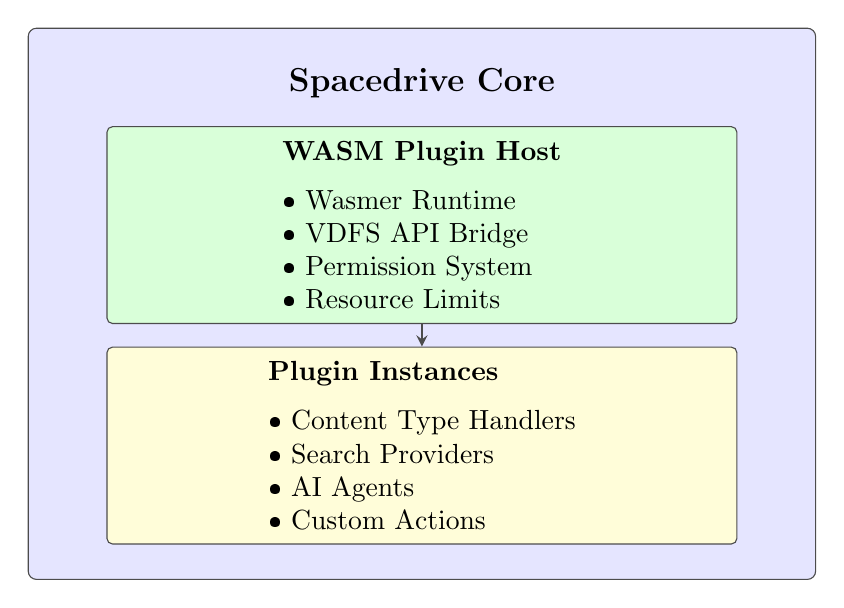
\begin{tikzpicture}[
    node distance=1.5cm,
    % Styles
    mainbox/.style={rectangle, draw=black!70, fill=blue!10, minimum width=10cm, minimum height=7cm, align=center, rounded corners=3pt},
    hostbox/.style={rectangle, draw=black!70, fill=green!15, minimum width=8cm, minimum height=2.5cm, align=left, rounded corners=2pt},
    instancebox/.style={rectangle, draw=black!70, fill=yellow!15, minimum width=8cm, minimum height=2.5cm, align=left, rounded corners=2pt},
    arrow/.style={->, >=stealth, thick, color=black!70}
]

% Main container
\node[mainbox] (core) at (0,0) {};
\node at (0,2.8) {\textbf{\large Spacedrive Core}};

% WASM Plugin Host
\node[hostbox] (host) at (0,1) {
    \textbf{WASM Plugin Host}\\[0.2cm]
    \textbullet\ Wasmer Runtime\\
    \textbullet\ VDFS API Bridge\\
    \textbullet\ Permission System\\
    \textbullet\ Resource Limits
};

% Plugin Instances
\node[instancebox] (instances) at (0,-1.8) {
    \textbf{Plugin Instances}\\[0.2cm]
    \textbullet\ Content Type Handlers\\
    \textbullet\ Search Providers\\
    \textbullet\ AI Agents\\
    \textbullet\ Custom Actions
};

% Arrow between boxes
\draw[arrow] (host.south) -- (instances.north);

\end{tikzpicture}
\caption{Spacedrive Core WASM Plugin Architecture: Sandboxed execution environment with unified API for all extension types.}
\label{fig:plugin-architecture}
\end{figure}

This architecture provides:
\begin{itemize}
    \item Complete sandboxing for all extensions
    \item Unified API for all plugin types
    \item Hot-reload capability for development
    \item Platform-independent distribution
\end{itemize}

\paragraph{Cloud Storage Integration}
Cloud storage providers (S3, Google Drive, Dropbox, etc.) are implemented as WASM plugins that leverage the OpenDAL library. This approach:
\begin{itemize}
    \item Maintains security through WASM sandboxing
    \item Enables hot-swappable cloud provider support
    \item Allows community-contributed storage backends
    \item Provides consistent API across all storage types
\end{itemize}


% --- SECTION 7: RESOURCE EFFICIENCY AND MOBILE CONSIDERATIONS ---
\section{Resource Efficiency and Mobile Considerations}
Spacedrive is designed to be a responsible citizen on user devices, particularly mobile platforms where battery life and storage are constrained.

\subsection{Adaptive Background Processing}
The system employs intelligent resource management to balance functionality with device performance:


\textbf{Intelligent Resource Management}

Spacedrive continuously monitors device conditions and automatically adjusts its resource usage to maintain optimal performance:

\textbf{Resource Monitoring}
\begin{itemize}[noitemsep, topsep=0pt]
 \item \textbf{Power Status}: Distinguishes between plugged-in and battery operation
 \item \textbf{Thermal Conditions}: Monitors device temperature and throttles when hot
 \item \textbf{Network Type}: Detects WiFi vs. cellular connections for data-conscious behavior
 \item \textbf{Device Type}: Adapts behavior for mobile vs. desktop environments
\end{itemize}

\textbf{Adaptive Behavior}
\begin{itemize}[noitemsep, topsep=0pt]
 \item \textbf{Battery Power}: Reduces CPU usage by 50\%, doubles sync intervals, minimizes background indexing
 \item \textbf{Thermal Pressure}: Dramatically reduces processing to prevent overheating
 \item \textbf{Cellular Connection}: Limits network bandwidth to 1MB/s, prioritizes critical operations
 \item \textbf{Background Mode}: Defers heavy operations until the user is actively using the app
\end{itemize}


\subsubsection{Platform-Specific Optimizations}

\textbf{iOS/iPadOS}:
- Background processing limited to 30-second windows when app backgrounded
- Incremental indexing during brief background execution periods
- Sync operations deferred until app returns to foreground

\textbf{Android}:
- Doze mode compatibility with intelligent scheduling around maintenance windows
- Adaptive sync frequency based on device usage patterns
- Background processing respects battery optimization settings

\textbf{Desktop Platforms}:
- Full background operation with thermal and power management
- CPU thread scaling based on available cores and current load
- Memory usage caps based on total system memory

\textbf{Bluetooth Discovery (Spacedrop)}:
- iOS/macOS: Native Core Bluetooth framework with user permission
- Android: BluetoothLeScanner APIs with location permission requirements
- Windows 10/11: WinRT Bluetooth LE APIs for proximity detection
- Linux: BlueZ D-Bus integration where available

\subsection{Storage Efficiency}
Spacedrive minimizes storage overhead through several strategies:

\subsubsection{Compact Database Design}


\textbf{Space-Optimized Database Design}

Spacedrive's database uses several techniques to minimize storage overhead while maintaining performance:

\textbf{Efficient Data Representation}
\begin{itemize}[noitemsep, topsep=0pt]
 \item \textbf{Compact Timestamps}: Unix epoch integers instead of text strings (4 bytes vs 20+ bytes)
 \item \textbf{Bitfield Metadata}: Common boolean properties packed into single integers
 \item \textbf{Relative Paths}: Store only the path relative to location, not full absolute paths
 \item \textbf{Reference-Based Content}: Link to shared content records rather than duplicating information
\end{itemize}

\textbf{Intelligent Thumbnail Management}
\begin{itemize}[noitemsep, topsep=0pt]
 \item \textbf{Progressive Quality}: Generate thumbnails in multiple sizes (tiny, small, medium, large) on demand
 \item \textbf{Modern Formats}: Use efficient compression (WebP, AVIF) while maintaining compatibility
 \item \textbf{Storage Only When Needed}: Generate thumbnails only for files that are actually viewed
\end{itemize}


\textbf{Database Compression}: SQLite databases use page-level compression, typically achieving 60-80\% space savings for metadata.

\textbf{Progressive Thumbnails}: Generate thumbnails on-demand in multiple sizes, storing only what's needed for current UI requirements.

\subsubsection{Memory Management}


\textbf{Memory-Efficient Query Processing Architecture}

Spacedrive employs sophisticated memory management strategies to handle large datasets efficiently:

\textbf{Streaming Query Execution}
\begin{itemize}[noitemsep, topsep=0pt]
 \item Large queries process results as streams rather than loading everything into memory
 \item Prevents memory exhaustion when working with millions of file entries
 \item Cached prepared statements eliminate repeated query compilation overhead
 \item Incremental result processing enables responsive UI even with massive datasets
\end{itemize}

\textbf{Intelligent Caching Strategy}
\begin{itemize}[noitemsep, topsep=0pt]
 \item LRU (Least Recently Used) cache for frequently accessed metadata
 \item Configurable cache size limits based on available system memory
 \item Automatic eviction of stale data to prevent memory bloat
 \item Hot data remains instantly accessible while cold data is fetched on demand
\end{itemize}

\textbf{Resource-Conscious Design}
\begin{itemize}[noitemsep, topsep=0pt]
 \item Query results transform directly into UI-ready objects without intermediate copying
 \item Error handling integrated into streaming pipeline for robust operation
 \item Memory usage scales with active operations, not total library size
\end{itemize}


\textbf{Streaming Operations}: Large queries use iterators rather than loading complete result sets into memory.

\textbf{Bounded Caches}: LRU caches for frequently accessed data with configurable size limits based on available memory.

\subsection{Network Efficiency}
Cross-device operations are optimized for both speed and data usage:

\subsubsection{Intelligent Sync Strategies}


\textbf{Connection-Aware Synchronization}

Spacedrive intelligently adapts its sync behavior based on the user's current network conditions:

\textbf{WiFi Connections}
\begin{itemize}[noitemsep, topsep=0pt]
 \item Full synchronization of all pending changes
 \item Unrestricted file transfers and metadata updates
 \item Background operations proceed at full capacity
\end{itemize}

\textbf{Cellular Connections}
\begin{itemize}[noitemsep, topsep=0pt]
 \item Priority-based sync focusing on critical changes first
 \item 10MB size limit for individual file transfers
 \item Metadata and small files synchronized immediately
\end{itemize}

\textbf{Metered Connections}
\begin{itemize}[noitemsep, topsep=0pt]
 \item Metadata-only synchronization to preserve data allowances
 \item File transfers deferred until unmetered connection available
 \item User can override for urgent transfers
\end{itemize}


\textbf{Connection-Aware Sync}: Automatically adjust sync behavior based on connection type and user preferences.

\textbf{Delta Sync}: Only transmit changed data rather than full file re-uploads.

\textbf{Compression}: Use zstd compression for metadata sync, achieving ~70\% reduction in network usage.

This resource-conscious design ensures Spacedrive provides powerful functionality without compromising device performance or user experience.


% --- SECTION 8: SECURITY AND PRIVACY MODEL ---
\section{Security and Privacy Model}

\begin{keytakeaways}
\begin{itemize}[noitemsep, topsep=0pt]
\item \textbf{Defense in Depth}: SQLCipher database encryption + ChaCha20 network keys + TLS 1.3 transport = comprehensive protection
\item \textbf{Zero-Knowledge Cloud}: Your Spacedrive Cloud instance cannot decrypt your data---only you have the keys
\item \textbf{Battle-Tested Security}: Protection against real attacks: NAS compromise, stolen devices, cloud breaches, and insider threats
\end{itemize}
\end{keytakeaways}

Spacedrive's architecture prioritizes user privacy and data security through comprehensive encryption, secure credential management, and a well-defined threat model designed for personal data scenarios.

\subsection{Data Protection at Rest}
All sensitive user data is encrypted using industry-standard cryptographic protocols:

\subsubsection{Library Database Encryption}
Each `.sdlibrary` directory employs transparent database encryption:

Library databases employ SQLCipher for transparent encryption at rest. Encryption keys are derived from user passwords using PBKDF2 with 100,000+ iterations and unique per-library salts. The unlocking process involves reading the salt, deriving the key, opening the encrypted database connection, and verifying access through a test query.

\textbf{Key derivation}: User passwords are strengthened using PBKDF2 with 100,000+ iterations and unique salts per library, providing strong protection against brute-force attacks.

\subsubsection{Network Identity Protection}
Device cryptographic keys are stored encrypted in the enhanced device configuration:

Network identity protection employs a layered approach: Ed25519 private keys are encrypted using ChaCha20-Poly1305 with keys derived through Argon2id from user passwords. Public keys remain in plaintext for identity verification. Decryption involves deriving the key using Argon2id parameters and salt, then decrypting the private key data.

\subsection{Network Security}
All network communications employ end-to-end encryption with perfect forward secrecy:

\subsubsection{Iroh QUIC Transport Security}
The Iroh networking stack provides multiple layers of security through secure connections that combine long-term device identity (Ed25519) with ephemeral session keys. Connection establishment involves a three-phase process: QUIC handshake with TLS 1.3, mutual device identity verification, and application-level key exchange for perfect forward secrecy.

\textbf{Transport Layer Security}: QUIC provides TLS 1.3 encryption for all network traffic, ensuring confidentiality and integrity.

\textbf{Application Layer Security}: Additional encryption using ephemeral keys provides perfect forward secrecy---compromising long-term device keys cannot decrypt past communications. This is particularly important for Spacedrop transfers, where each session uses completely ephemeral ECDH key exchange, ensuring that even if device keys are later compromised, past file transfers remain secure.

\subsection{Credential Management}
Spacedrive employs a secure credential storage system for cloud service integration:


\textbf{Secure Credential Vault Architecture}

Spacedrive implements a multi-layered credential protection system for cloud service integration:

\textbf{Master Key Derivation}
\begin{itemize}[noitemsep, topsep=0pt]
 \item User password transformed into cryptographically strong master key using PBKDF2
 \item Unique salt per credential vault prevents rainbow table attacks
 \item Key stretching with 100,000+ iterations provides brute-force resistance
\end{itemize}

\textbf{Individual Credential Protection}
\begin{itemize}[noitemsep, topsep=0pt]
 \item Each credential encrypted separately using ChaCha20-Poly1305 authenticated encryption
 \item Unique random nonce for each encryption operation ensures semantic security
 \item Comprehensive metadata tracking: service name, creation time, last access
\end{itemize}

\textbf{Storage and Lifecycle Management}
\begin{itemize}[noitemsep, topsep=0pt]
 \item Encrypted credentials stored in secure key-value mapping by service name
 \item Automatic timestamp tracking for security auditing and credential rotation
 \item Zero plaintext credential storage---everything encrypted at rest
\end{itemize}


\textbf{Platform Integration}: On supported platforms (macOS Keychain, Windows Credential Manager, Linux Secret Service), credentials are additionally protected by the OS credential store.

\subsection{Threat Model}
Spacedrive's security design addresses the following threat scenarios:

\subsubsection{Local Device Compromise}
\textbf{Threat}: Unauthorized physical access to user device.

\textbf{Mitigation}:
- Database encryption renders `.sdlibrary` directories unreadable without password
- Network keys encrypted separately, requiring password for decryption
- No plaintext credentials stored on disk

\subsubsection{Network Eavesdropping}
\textbf{Threat}: Passive monitoring of network communications.

\textbf{Mitigation}:
- All communications encrypted with TLS 1.3 via QUIC
- Perfect forward secrecy prevents retroactive decryption
- Device fingerprints prevent MITM attacks during pairing

\subsubsection{Cloud Service Compromise}
\textbf{Threat}: Breach of connected cloud storage providers.

\textbf{Mitigation}:
- Spacedrive never stores user data in cloud services---only metadata indices
- Cloud credentials encrypted locally, not shared with Spacedrive services
- Content addressing enables detection of tampered files

\subsubsection{Malicious Spacedrive Instance}
\textbf{Threat}: Compromised or malicious Spacedrive installation.

\textbf{Mitigation}:
- Libraries are portable and can be moved between trusted installations
- Audit logs provide complete history of all operations
- Action preview system prevents unauthorized operations

\subsubsection{Practical Attack Scenarios}
To illustrate the robustness of Spacedrive's security model, consider these realistic attack scenarios:

\textbf{Scenario 1: NAS Compromise and File Replacement}

\emph{Attack}: An attacker gains access to a user's NAS and replaces legitimate files with malicious versions, attempting to propagate malware across the user's device ecosystem.

\emph{Spacedrive Defense}:
\begin{itemize}[noitemsep, topsep=0pt]
\item Content addressing via BLAKE3 hashes immediately detects file modifications---the replaced files will have different hashes than the indexed versions
\item The integrity verification system flags discrepancies during the next scan, alerting the user to potential tampering
\item Version history tracking shows the exact timestamp of unauthorized modifications
\item Quarantine mechanisms prevent automatic synchronization of suspicious files to other devices
\item The audit log creates a forensic trail showing which files were modified and when
\end{itemize}

\textbf{Scenario 2: Stolen Laptop with Sensitive Photo Library}

\emph{Attack}: A laptop containing a Spacedrive library with sensitive personal photos is stolen. The attacker attempts to access the photo collection and extract metadata about locations and people.

\emph{Spacedrive Defense}:
\begin{itemize}[noitemsep, topsep=0pt]
\item SQLCipher encryption on the library database prevents access without the user's password
\item Photo metadata and AI-generated embeddings remain encrypted at rest
\item Even with physical disk access, the attacker cannot:
  - View photo thumbnails (encrypted in cache)
  - Access location data from EXIF metadata (encrypted in database)
  - Extract face recognition data or object detection results (encrypted embeddings)
\item The 100,000+ iteration PBKDF2 key derivation makes brute-force attacks computationally infeasible
\end{itemize}

\textbf{Scenario 3: Compromised Cloud Storage Credentials}

\emph{Attack}: An attacker obtains a user's cloud storage credentials through a phishing attack and attempts to inject malicious files into the user's Spacedrive-managed cloud volumes.

\emph{Spacedrive Defense}:
\begin{itemize}[noitemsep, topsep=0pt]
\item Spacedrive's credential vault remains secure---the attacker only has cloud credentials, not the Spacedrive master password
\item Content validation during cloud synchronization detects unexpected file additions
\item The volume classification system isolates cloud storage from local trusted volumes
\item File injection attempts are logged in the audit system with source attribution
\item Users can revoke cloud volume access instantly without affecting local data
\item Optional two-factor authentication on cloud volume operations provides additional protection
\end{itemize}

\textbf{Scenario 4: Insider Threat in Collaborative Team}

\emph{Attack}: A disgruntled employee on a design team attempts to exfiltrate proprietary assets and delete project files before leaving the company.

\emph{Spacedrive Defense}:
\begin{itemize}[noitemsep, topsep=0pt]
\item RBAC system restricts the employee to their assigned role permissions---they may have "Contributor" access allowing edits but not bulk deletions
\item The Action System's preview capability flags suspicious bulk operations for administrative review
\item Every file access and operation is logged in the immutable audit trail with full attribution (user, device, timestamp)
\item Data Loss Prevention (DLP) policies can detect and block unusual download patterns or transfers to external devices
\item Time-based access controls automatically revoke permissions at employment end date
\item The planned undo capability would allow administrators to instantly reverse any destructive actions
\item Cryptographic device attestation ensures actions can only originate from company-managed devices
\end{itemize}

\textbf{Scenario 5: Supply Chain Attack on Enterprise Deployment}

\emph{Attack}: An attacker attempts to compromise an enterprise Spacedrive deployment by injecting malicious code into a third-party integration or storage driver.

\emph{Spacedrive Defense}:
\begin{itemize}[noitemsep, topsep=0pt]
\item Containerized deployment isolates each component with strict network policies
\item All actions flow through the centralized Action System, preventing direct database manipulation
\item Cryptographic signatures on all deployed components ensure integrity
\item The audit system's append-only design prevents log tampering to hide malicious activity
\item Storage abstraction layer validates all operations against expected patterns
\item Regular security scanning of container images and dependencies
\item Option for air-gapped deployment in high-security environments
\end{itemize}

\subsection{Certificate Pinning and API Security}
\subsubsection{Cloud Provider Certificate Pinning}
Spacedrive implements robust certificate pinning for all cloud storage provider connections:

\textbf{Implementation Strategy}:
\begin{itemize}[noitemsep, topsep=0pt]
\item Pin both leaf certificates and intermediate CA certificates for major providers
\item Maintain backup pins for certificate rotation scenarios
\item Implement graceful fallback with user notification if pins fail
\item Regular updates through secure channels for pin refreshes
\end{itemize}

\textbf{Provider-Specific Handling}:
\begin{itemize}[noitemsep, topsep=0pt]
\item \textbf{Google Drive}: Pin GTS root and intermediate certificates
\item \textbf{Dropbox}: Pin DigiCert certificates with rotation monitoring
\item \textbf{OneDrive}: Pin Microsoft PKI infrastructure certificates
\item \textbf{S3-Compatible}: User-configurable pins for self-hosted instances
\end{itemize}

\subsection{Rate Limiting and Abuse Prevention}
\subsubsection{Multi-Layer Rate Limiting Architecture}
Spacedrive implements comprehensive rate limiting to prevent abuse while maintaining performance:

\textbf{API Rate Limiting}:
\begin{itemize}[noitemsep, topsep=0pt]
\item Per-device token bucket algorithm with configurable rates
\item Separate limits for read operations (1000/min) and write operations (100/min)
\item Exponential backoff for repeated limit violations
\item Priority queuing for critical operations during limit conditions
\end{itemize}

\textbf{Network-Level Protection}:
\begin{itemize}[noitemsep, topsep=0pt]
\item Connection rate limiting per IP address (10 new connections/minute)
\item Bandwidth throttling for suspected abuse patterns
\item Automatic blacklisting for persistent violators
\item DDoS mitigation through connection pooling limits
\end{itemize}

\textbf{Operation-Level Safeguards}:
\begin{itemize}[noitemsep, topsep=0pt]
\item Bulk operation limits (max 1000 files per action)
\item Concurrent job restrictions based on device capabilities
\item Smart scheduling to prevent resource exhaustion
\item User-configurable limits for shared libraries
\end{itemize}

\subsection{Audit Log Immutability}
\subsubsection{Cryptographic Audit Trail}
The audit log system ensures tamper-proof record keeping through cryptographic guarantees:

\textbf{Chain-Based Integrity}:
\begin{itemize}[noitemsep, topsep=0pt]
\item Each audit entry includes hash of previous entry
\item Merkle tree structure for efficient verification
\item Periodic checkpoint hashes signed with device keys
\item Distributed verification across paired devices
\end{itemize}

\textbf{Implementation Details}:
\begin{lstlisting}[language=Rust, caption={Audit log entry structure with cryptographic chaining}]
pub struct AuditEntry {
    pub id: Uuid,
    pub timestamp: DateTime<Utc>,
    pub action: ActionType,
    pub device_id: DeviceId,
    pub details: serde_json::Value,
    pub previous_hash: Blake3Hash,
    pub entry_hash: Blake3Hash,
}

impl AuditEntry {
    pub fn compute_hash(&self) -> Blake3Hash {
        let mut hasher = blake3::Hasher::new();
        hasher.update(&self.timestamp.to_rfc3339().as_bytes());
        hasher.update(&self.action.to_bytes());
        hasher.update(&self.device_id.as_bytes());
        hasher.update(&self.details.to_string().as_bytes());
        hasher.update(&self.previous_hash.as_bytes());
        hasher.finalize()
    }
}
\end{lstlisting}

\textbf{Verification Process}:
\begin{itemize}[noitemsep, topsep=0pt]
\item Background verification runs periodically
\item Cross-device hash comparison during sync
\item Immediate alerts for chain violations
\item Export capability for external audit systems
\end{itemize}

\subsection{Spacedrive Cloud Service Privacy Model}
The managed Spacedrive Cloud Service treats privacy as a fundamental design principle, not an afterthought:

\subsubsection{End-to-End Encryption Architecture}
The Cloud Core instance runs the standard Spacedrive software with no special privileges or backdoors:

\textbf{Zero-Knowledge Design}:
\begin{itemize}[noitemsep, topsep=0pt]
 \item User libraries remain encrypted at rest using keys derived from user passwords
 \item Spacedrive Inc. has no access to user encryption keys or passwords
 \item All file transfers use end-to-end encryption via the Iroh protocol
 \item Cloud Core instances cannot decrypt user data without explicit user authentication
\end{itemize}

\textbf{Cryptographic Isolation}:
\begin{itemize}[noitemsep, topsep=0pt]
 \item Each Cloud Core runs in an isolated container with unique cryptographic identity
 \item Network policies enforce that only paired devices can communicate
 \item No shared infrastructure between different user instances
 \item Complete data isolation at storage, network, and compute layers
\end{itemize}

\subsubsection{Operational Security}
Infrastructure access is strictly controlled and audited:

\textbf{Administrative Access}:
\begin{itemize}[noitemsep, topsep=0pt]
 \item No direct access to user containers or data volumes
 \item Administrative operations limited to resource management and health monitoring
 \item All infrastructure access logged and audited
 \item User data remains encrypted even during backup operations
\end{itemize}

\textbf{Data Retention and Deletion}:
\begin{itemize}[noitemsep, topsep=0pt]
 \item User data is permanently deleted within 30 days of account closure
 \item Cryptographic erasure ensures data cannot be recovered
 \item Users can export their entire library before deletion
 \item No data mining or analysis of user content
\end{itemize}

\subsection{Privacy-Preserving AI}
The AI-native architecture maintains privacy through multiple mechanisms:


\textbf{Flexible AI Provider Selection for Privacy Control}

Spacedrive supports multiple AI deployment models to balance privacy, performance, and capability:

\textbf{Local AI Processing (Maximum Privacy)}
\begin{itemize}[noitemsep, topsep=0pt]
 \item Integrates with Ollama for completely local AI model execution
 \item User data never leaves the device---complete privacy preservation
 \item Configurable endpoint and model selection for different AI capabilities
 \item Works offline once models are downloaded
\end{itemize}

\textbf{Self-Hosted Solutions (Organizational Control)}
\begin{itemize}[noitemsep, topsep=0pt]
 \item Custom AI infrastructure under user or organization control
 \item Flexible authentication options for enterprise deployment
 \item Complete control over data processing and model selection
 \item Ideal for organizations with specific privacy or compliance requirements
\end{itemize}

\textbf{Cloud AI Services (Enhanced Capabilities)}
\begin{itemize}[noitemsep, topsep=0pt]
 \item Access to state-of-the-art models from major AI providers
 \item Encrypted API key storage with comprehensive privacy policy tracking
 \item Transparent data processing terms presented to users for informed consent
 \item Metadata-only transmission---file contents remain local
\end{itemize}


\textbf{Local Processing}: Default to local AI models (Ollama) that never transmit user data externally.

\textbf{Metadata-Only Cloud Processing}: When using cloud AI services, only file metadata (names, types, sizes) are transmitted---never file contents.

\textbf{User Control}: Complete transparency about which AI provider processes which data, with granular user control over privacy vs. capability trade-offs.

\subsection{Balancing Privacy and Public Sharing}

Spacedrive's security model accommodates both zero-knowledge privacy and public content sharing through its library-based architecture.

\subsubsection{Per-Library Encryption Policy}

Each library maintains independent encryption settings:

\begin{itemize}
    \item \textbf{Private Libraries} (default): Full SQLCipher encryption at rest
    \item \textbf{Public Libraries} (opt-in): Unencrypted for web serving
    \item \textbf{Hybrid Libraries}: Encrypted with selective public locations
\end{itemize}

\begin{lstlisting}[language=Rust, caption=Library encryption configuration]
pub struct LibraryConfig {
    pub encryption: EncryptionMode,
    pub public_sharing: PublicSharingConfig,
}

pub enum EncryptionMode {
    /// Full encryption (default)
    Encrypted { key_derivation: Argon2id },
    /// No encryption (for public content)
    Unencrypted,
    /// Encrypted with public locations
    Hybrid { public_locations: Vec<LocationId> },
}

pub struct PublicSharingConfig {
    /// Which core serves public content
    pub hosting_core: CoreIdentity,
    /// Custom domain (if any)
    pub custom_domain: Option<String>,
    /// Access control rules
    pub access_rules: Vec<AccessRule>,
}
\end{lstlisting}

\subsubsection{Secure Public Sharing Workflow}

Users can share content publicly without compromising private data:

\begin{enumerate}
    \item Create a dedicated public library or location
    \item Configure which core hosts public content (cloud or self-hosted)
    \item Move/copy files to public locations
    \item Share generated URLs with recipients
    \item Private libraries remain fully encrypted throughout
\end{enumerate}

\subsubsection{Implementation Considerations}

This dual-mode approach ensures:

\begin{itemize}
    \item \textbf{Clear Boundaries}: Users explicitly choose what becomes public
    \item \textbf{No Encryption Downgrade}: Private libraries cannot be converted to public
    \item \textbf{Audit Trail}: All public sharing actions are logged
    \item \textbf{Revocable Access}: Public files can be made private instantly
    \item \textbf{Hosting Flexibility}: Any core can serve public content with proper setup
\end{itemize}

\paragraph{Security Implications}
The system maintains security through isolation:

\begin{itemize}
    \item Public and private data never mix within a library
    \item Encryption keys are never exposed to hosting infrastructure
    \item Access tokens are scoped to specific libraries and operations
    \item Public URLs use capability-based security (unguessable paths)
\end{itemize}

By making encryption optional but enabled by default, Spacedrive provides flexibility for content creators and enterprises while maintaining strong privacy guarantees for personal data.


% --- SECTION 9: PRACTICAL CONFLICT RESOLUTION ---
\section{Practical Conflict Resolution}
While the simulation engine prevents operational conflicts before they occur, synchronization conflicts can still arise when multiple devices modify the same data concurrently. Library Sync's domain separation significantly reduces these conflicts, but when they do occur---particularly in the User Metadata domain---the system provides transparent, user-controlled conflict resolution that maintains data integrity while preserving user intent.

\subsection{Metadata Conflict Scenarios}
The most common conflicts occur when multiple devices modify the same content metadata simultaneously:

\subsubsection{Tag Conflicts}
\textbf{Scenario}: User adds tag "vacation" on Device A while simultaneously adding tag "family" on Device B to the same photo.

\textbf{Resolution Strategy}: Union merge with conflict notification, leveraging the richly-structured tag system (Section 3.3):

\textbf{Intelligent Tag Conflict Resolution Process}

When tag conflicts occur, Spacedrive follows a sophisticated resolution process:

\textbf{Detection Phase}
\begin{itemize}[noitemsep, topsep=0pt]
 \item System identifies when the same file has been tagged differently on multiple devices
 \item Compares tag sets to determine if there's actual overlap or genuine conflict
 \item Analyzes tag hierarchies to identify if tags are related (e.g., both are children of the same parent tag)
 \item Generates comprehensive conflict context for decision-making
\end{itemize}

\textbf{Resolution Strategy}
\begin{itemize}[noitemsep, topsep=0pt]
 \item \textbf{Union Merge}: Automatically combines all tags from both devices
 \item \textbf{Conflict Notification}: Creates detailed notification explaining what was merged
 \item \textbf{User Transparency}: Provides complete visibility into the resolution process
\end{itemize}

\textbf{Outcome Tracking}
\begin{itemize}[noitemsep, topsep=0pt]
 \item Records timestamp and source of each tag for future reference
 \item Enables user to review and modify the automatic resolution if needed
 \item Maintains audit trail of all conflict resolution decisions
\end{itemize}


\textbf{User Experience}:
- Tags are automatically combined: "vacation, family"
- User receives notification: "Combined tags for sunset.jpg: added 'vacation' and 'family' from different devices"
- User can review and modify the combined tags if needed

\begin{figure}[h]
\centering
\begin{tikzpicture}[
    node distance=1.8cm,
    auto,
    % Styles
    device/.style={rectangle, rounded corners, draw=black!70, fill=blue!15, minimum width=2.5cm, minimum height=1cm, align=center},
    conflict/.style={circle, draw=red!70, fill=red!15, minimum width=2cm, align=center},
    process/.style={rectangle, rounded corners, draw=black!70, fill=green!15, minimum width=3.5cm, minimum height=1.2cm, align=center},
    result/.style={rectangle, rounded corners, draw=black!70, fill=yellow!15, minimum width=3cm, minimum height=1cm, align=center},
    notification/.style={rectangle, rounded corners, draw=orange!70, fill=orange!15, minimum width=4cm, minimum height=1cm, align=center},
    arrow/.style={->, >=stealth, thick},
    conflictarrow/.style={->, >=stealth, thick, red},
    label/.style={font=\scriptsize, fill=white, inner sep=2pt}
]
    % Devices
    \node[device] (deviceA) {Device A\\
    \scriptsize Tags: "vacation"};

    \node[device, right=3cm of deviceA] (deviceB) {Device B\\
    \scriptsize Tags: "family"};

    % Conflict Detection
    \node[conflict, below=2cm of $(deviceA)!0.5!(deviceB)$] (conflict) {Conflict\\Detected};

    % Resolution Process
    \node[process, below=of conflict] (resolution) {\textbf{Resolution Engine}\\
    \scriptsize
    • Compare tag sets\\
    • Apply union merge\\
    • Generate notification};

    % Result
    \node[result, below=of resolution] (merged) {Merged Result\\
    \scriptsize Tags: "vacation, family"};

    % User Notification
    \node[notification, right=of resolution] (notify) {\textbf{User Notification}\\
    \scriptsize
    "Combined tags from Device A \& B\\
    for sunset.jpg"};

    % Arrows
    \draw[conflictarrow] (deviceA) -- node[label, left] {Same file\\modified} (conflict);
    \draw[conflictarrow] (deviceB) -- node[label, right] {Same file\\modified} (conflict);
    \draw[arrow] (conflict) -- (resolution);
    \draw[arrow] (resolution) -- (merged);
    \draw[arrow] (resolution) -- (notify);

    % Sync arrows
    \draw[arrow, dashed, bend left=30] (merged.west) to node[label, left] {Sync back} (deviceA.south);
    \draw[arrow, dashed, bend right=30] (merged.east) to node[label, right] {Sync back} (deviceB.south);

    % Annotations
    \node[font=\tiny, text width=3cm, below=0.3cm of merged] {Both devices receive\\the merged tags};
\end{tikzpicture}
\caption{Tag Conflict Resolution: Union merge strategy automatically combines tags from multiple devices while notifying the user of the resolution.}
\label{fig:tag-conflict-resolution}
\end{figure}

\subsubsection{Rating Conflicts}
\textbf{Scenario}: Photo rated 4 stars on Device A, 5 stars on Device B.

\textbf{Resolution Strategy}: Last-writer-wins with user notification:


\textbf{Rating Conflict Resolution: Last-Writer-Wins Strategy}

For rating conflicts, Spacedrive uses a temporal resolution approach:

\textbf{Conflict Scenario}: Photo rated differently on multiple devices (e.g., 4 stars vs. 5 stars)

\textbf{Resolution Logic}
\begin{itemize}[noitemsep, topsep=0pt]
 \item \textbf{Timestamp Comparison}: System examines when each rating was applied
 \item \textbf{Most Recent Wins}: The more recent rating is automatically selected
 \item \textbf{Clear Attribution}: User notification specifies which device's rating was chosen and when
\end{itemize}

\textbf{User Experience}
\begin{itemize}[noitemsep, topsep=0pt]
 \item Automatic resolution without user intervention required
 \item Transparent notification: "sunset.jpg rating conflict resolved: using 5 stars (most recent)"
 \item User can manually override the automatic choice if they disagree with the outcome
\end{itemize}


\textbf{User Experience}:
- Most recent rating wins automatically
- Notification: "sunset.jpg rating conflict resolved: using 5 stars (most recent)"
- User can manually change rating if they disagree

\subsection{Advanced Conflict Scenarios}
\subsubsection{Complex Metadata Conflicts}
\textbf{Scenario}: User creates custom metadata field "project" with value "website" on Device A, while Device B creates the same field with value "portfolio".

\textbf{Intelligent Custom Metadata Conflict Resolution}

When users create conflicting custom metadata on different devices, Spacedrive provides sophisticated resolution assistance:

\textbf{Conflict Analysis}
\begin{itemize}[noitemsep, topsep=0pt]
 \item System identifies the specific metadata field and conflicting values
 \item Analyzes value types to determine if combination is possible
 \item Generates context-aware resolution suggestions based on conflict nature
\end{itemize}

\textbf{Smart Resolution Options}
\begin{itemize}[noitemsep, topsep=0pt]
 \item \textbf{Compatible Values}: For string conflicts, offers to use either value, combine them, or create custom resolution
 \item \textbf{Type Mismatches}: When data types differ, provides clear choice between local/remote values or custom entry
 \item \textbf{Contextual Suggestions}: System provides reasoning for each resolution option
\end{itemize}

\textbf{User Experience}
\begin{itemize}[noitemsep, topsep=0pt]
 \item Clear presentation of conflict: "project field conflicts: 'website' vs 'portfolio'"
 \item Multiple resolution choices: use either value, combine as "website, portfolio", or enter custom value
 \item One-time decision with preference learning for similar future conflicts
 \item Complete transparency about which device contributed each value
\end{itemize}

\textbf{User Experience}:
- System detects incompatible values for "project" field
- Presents clear options: "website", "portfolio", "website, portfolio", or custom value
- User makes one-time decision, system remembers preference for similar conflicts

\subsection{Conflict Prevention}
Spacedrive employs several strategies to minimize conflicts before they occur:

\subsubsection{Optimistic Locking}
\textbf{Optimistic Metadata Locking Strategy}

To prevent simultaneous metadata modifications that could lead to conflicts, Spacedrive employs a lightweight locking mechanism:

\textbf{Lock Characteristics}
\begin{itemize}[noitemsep, topsep=0pt]
 \item \textbf{Short Duration}: 30-second locks prevent long-term resource blocking
 \item \textbf{Field-Specific}: Locks target specific metadata fields, not entire files
 \item \textbf{Device Attribution}: Clear identification of which device holds each lock
 \item \textbf{Automatic Expiration}: Locks expire automatically to prevent deadlocks
\end{itemize}

\textbf{Cross-Device Coordination}
\begin{itemize}[noitemsep, topsep=0pt]
 \item Lock acquisition broadcasts to all connected devices in the library
 \item Other devices receive immediate notification and defer their edits
 \item Graceful handling of network interruptions during lock operations
 \item Automatic retry mechanisms for failed lock acquisitions
\end{itemize}

\textbf{User Experience Benefits}
\begin{itemize}[noitemsep, topsep=0pt]
 \item Prevents frustrating conflicts from simultaneous editing
 \item Near-instant feedback when metadata modification is blocked
 \item Transparent handling—users don't need to understand the locking mechanism
 \item Reliable metadata consistency across all devices
\end{itemize}

\subsubsection{Real-time Conflict Notifications}
When conflicts do occur, users receive immediate, actionable notifications:

\textbf{User-Friendly Conflict Notification System}

Spacedrive provides comprehensive, actionable notifications when conflicts occur and are resolved:

\textbf{Notification Structure}
\begin{itemize}[noitemsep, topsep=0pt]
 \item \textbf{Clear Titles}: Descriptive headings like "Photo tags updated on both devices"
 \item \textbf{Detailed Descriptions}: Specific information about what was changed or merged
 \item \textbf{Affected Files List}: Complete inventory of files impacted by the conflict resolution
 \item \textbf{Action Options}: Clear next steps like "Tap to review" or "Changes automatically applied"
\end{itemize}

\textbf{Example Notification}
\begin{itemize}[noitemsep, topsep=0pt]
 \item \textbf{Title}: "Metadata synchronized"
 \item \textbf{Description}: "Combined tags from iPhone and MacBook for 3 photos"
 \item \textbf{Affected Files}: sunset.jpg, beach.jpg, vacation.mp4
 \item \textbf{User Action}: "Review changes" (optional)
 \item \textbf{Status}: Auto-resolved with timestamp for audit trail
\end{itemize}

\textbf{Transparency and Control}
\begin{itemize}[noitemsep, topsep=0pt]
 \item Complete visibility into what conflicts occurred and how they were resolved
 \item Clear indication of automatic vs. manual resolution requirements
 \item Historical timestamp for tracking when conflicts were addressed
 \item Optional review actions for users who want to verify or modify automatic resolutions
\end{itemize}

This transparent, user-controlled approach to conflict resolution ensures that users maintain complete control over their metadata while benefiting from seamless synchronization across devices.


% --- SECTION 10: CONCLUSION ---
\section{Conclusion}

\begin{keytakeaways}
\begin{itemize}[noitemsep, topsep=0pt]
\item \textbf{Vision Realized}: Enterprise-grade distributed file management made accessible to everyone through careful engineering
\item \textbf{Production Proven}: Real implementation handling millions of files with sub-100ms response times validates every architectural decision
\item \textbf{Future Ready}: Solid foundation for AI agents, federated learning, and the next paradigm of human-computer interaction
\end{itemize}
\end{keytakeaways}

Spacedrive represents a fundamental rethinking of personal file management, demonstrating that sophisticated distributed systems capabilities can be made accessible to individual users through careful architectural design and practical engineering choices. Through our implementation, we have shown that personal data management can evolve beyond simple file browsers to become intelligent, distributed systems that respect user ownership while providing enterprise-level capabilities, embodying the principles of local-first software~\cite{kleppmann_localfirst_2019} and ubiquitous computing~\cite{weiser_ubiquitous_1991}.

\subsection{Key Contributions and Real-World Impact}
This work transforms personal file management through five architectural innovations: AI-native design for natural language operations, universal file addressing that transcends device boundaries, immediate metadata capabilities for every file, domain-separated synchronization without consensus complexity, and performance-aware deduplication for consumer hardware.

The practical impact is immediate and measurable. Users manage millions of files across dozens of devices through a single interface, eliminating storage waste while maintaining sub-second response times. Data remains portable, privacy is preserved through local-first design, and AI enhancement comes without sacrificing user control. Our production Rust implementation validates these concepts at scale, proving that enterprise capabilities can indeed be delivered with consumer-friendly simplicity.

\subsection{System Integration}
These individual innovations combine synergistically to create capabilities greater than the sum of their parts. The Library abstraction makes backup and migration trivial (copy a directory), while SdPath enables seamless operations across that distributed storage. Content addressing works transparently with the sync system to maintain deduplication relationships even as files move between devices. The Temporal-Semantic Search architecture leverages both the content addressing and metadata systems to provide semantic discovery at traditional keyword search speeds.

\subsection{Validation in Production}
Spacedrive's architecture has been validated through production implementation in Rust, demonstrating that these concepts work reliably in practice. The system handles millions of files across multiple devices while maintaining sub-second response times for user operations. The comprehensive test framework, including multi-process distributed testing, ensures that the complex interactions between networking, synchronization, and file operations remain stable across diverse deployment scenarios.

\subsection{Future Work and Roadmap}
The architectural foundation laid by Spacedrive opens concrete paths for near-term enhancements and long-term research directions. Our immediate roadmap focuses on extending the AI capabilities to support complex multi-step workflows, such as "organize all vacation photos by year and location, then create albums for each trip." This involves expanding the Action system to support workflow composition while maintaining the same security and reversibility guarantees. Parallel to this, we are developing intelligent content analysis pipelines that leverage both local and cloud models to automatically extract semantic information from files---identifying people in photos, extracting key topics from documents, and understanding relationships between files based on content rather than just metadata.

In the medium term, our research agenda includes three major initiatives. First, we are exploring federated learning approaches that would allow users to benefit from collective intelligence about file organization patterns while maintaining complete privacy---the system would learn from aggregate behaviors without ever exposing individual file information. Second, we are developing advanced storage tiering algorithms that combine AI predictions with real-time access patterns to automatically move files between fast local storage, slower archives, and cloud services based on predicted access likelihood and user-defined cost constraints. Third, we are investigating cross-Library content discovery mechanisms that would allow users to identify duplicate content across different Libraries (perhaps owned by family members or team members) while maintaining the strong isolation guarantees that make Libraries portable and secure.

The longer-term vision extends Spacedrive beyond personal file management into a platform for personal AI agents that understand and manage all aspects of a user's digital life. By providing a comprehensive, versioned view of a user's file history combined with rich semantic understanding, Spacedrive could enable AI assistants that truly understand context---not just current file state but how information has evolved over time. This temporal understanding, combined with the robust Action system, would allow AI agents to perform complex organizational tasks with confidence, knowing that all actions are reversible and auditable. The architecture's emphasis on user control ensures that as these AI capabilities grow more sophisticated, users retain ultimate authority over their data, with all AI operations remaining transparent, explainable, and reversible.

\subsection{Broader Implications}
Spacedrive proves that the dichotomy between intuitive, user-centric applications and powerful, secure enterprise systems is a false one. Through careful domain separation, a local-first security model, and an architecture built for scale, we have demonstrated that it is possible to build a single platform that serves the needs of both individual users and large organizations. The key insight is that by starting with a foundation of user empowerment and data sovereignty, we create a system that naturally scales up to enterprise requirements while maintaining the simplicity and control that individual users demand.

This approach suggests a path forward for personal computing that moves beyond the current model of data scattered across incompatible cloud services toward truly user-controlled, portable, and intelligent data management. The native cloud service model presented in Section 7 is a clear manifestation of this principle, proving that cloud convenience does not have to come at the cost of architectural integrity or user control. By treating the cloud as just another trusted peer, Spacedrive offers a viable hybrid model for the future of personal data. By treating personal data as a unified library rather than a collection of disconnected files, users gain both the simplicity of traditional file management and the power of modern distributed systems.

Spacedrive's architecture provides a robust foundation for the next generation of computing---one that bridges personal and enterprise needs seamlessly. Whether serving an individual creator, a small team, or a global enterprise, the platform delivers the same core promise: unified access to all data, intelligent assistance without sacrificing control, and a user experience that makes powerful capabilities feel effortless. This is not just the future of file management, but a new paradigm for how humans and organizations interact with their digital assets at any scale.


% --- ACKNOWLEDGMENTS ---
\begin{acks}
We thank the open-source community, particularly the developers of the Rust programming language and its ecosystem, including the Tauri, Iroh, Tokio and SeaORM projects, whose work provided the foundation for this research.

The authors acknowledge the use of generative AI tools for assistance in drafting and refining the prose of this whitepaper. The core architectural concepts, technical details, and design are the original work of the authors, who take full responsibility for the content and accuracy of this paper.
\end{acks}


% --- GLOSSARY ---
\appendix
\section{Glossary of Terms}

\subsection*{Core Concepts}

\textbf{Action}: A pre-visualized, durable file operation that can be simulated before execution. Actions are the primary way users interact with files in Spacedrive.

\textbf{CAS (Content-Addressed Storage)}: A storage system where data is identified by its content hash rather than location, enabling automatic deduplication.

\textbf{Entry}: The fundamental data unit in Spacedrive representing any filesystem entity (file or directory) with immediate metadata capabilities.

\textbf{Library}: A portable, self-contained \texttt{.sdlibrary} directory containing a complete Spacedrive database, configuration, and metadata for a user's data ecosystem.

\textbf{Temporal-Semantic Search}: Spacedrive's two-stage hybrid search architecture combining temporal-first filtering with vector-enhanced semantic discovery.

\textbf{SdPath}: Spacedrive's universal path abstraction that transparently addresses files across devices, volumes, and cloud storage.

\textbf{VDFS (Virtual Distributed File System)}: A unified index of all user data across devices while keeping files in their original locations.

\subsection*{Technical Components}

\textbf{Content Identity}: A unique identifier based on file content hash that tracks all instances of identical content across the Library.

\textbf{CRDT (Conflict-free Replicated Data Type)}: A data structure that automatically resolves conflicts in distributed systems. Note: Spacedrive v1 attempted a custom CRDT implementation that proved overly complex. V2 replaced this with a simpler domain separation approach (see Section~\ref{sec:library-sync}).

\textbf{FTS (Full-Text Search)}: Traditional keyword-based search capability integrated into Spacedrive's Temporal-Semantic Search system.

\textbf{Phantom Path}: A special SdPath variant representing files that may not currently exist but are referenced in the Library index.

\textbf{Virtual Sidecar System}: A system for managing derivative data (e.g., thumbnails, OCR text, transcripts) associated with a file Entry. These sidecar files are stored within the Spacedrive Library and linked to the original file via the VDFS index, ensuring the original file is never modified.

\textbf{Volume}: Any storage location (local drive, network mount, cloud service) that Spacedrive can access and index.

\textbf{OpenDAL}: Open Data Access Layer, providing unified access to cloud storage services.

\textbf{ContentKind}: Semantic categorization system that groups files into 17 intuitive categories (Image, Video, Code, etc.) beyond traditional MIME types.

\textbf{File Type System}: Advanced multi-method file identification combining extension matching, magic byte detection, and content analysis with confidence scoring.

\subsection*{Architecture \& Deployment}

\textbf{Daemon}: A background service that hosts the Spacedrive core engine, providing persistent state management and enabling multiple clients to connect concurrently.

\textbf{Embedded Mode}: Deployment model where the core is directly linked into the application binary, used for mobile apps and standalone distributions.

\textbf{IPC (Inter-Process Communication)}: The mechanism for client-daemon communication using Unix domain sockets or named pipes with a JSON-RPC protocol.

\textbf{WASM Plugin}: WebAssembly-based extension running in a sandboxed environment.

\textbf{Integration}: WASM plugin providing system integration (e.g., cloud storage).

\subsection*{Synchronization \& Networking}

\textbf{Library Sync}: Spacedrive's intelligent synchronization system that keeps Libraries consistent across all devices by separating concerns into three domains:
\begin{itemize}[noitemsep, topsep=0pt]
  \item \textit{Index Sync}: Maintains consistent filesystem state across devices
  \item \textit{User Metadata Sync}: Handles tags, ratings, and other user-generated metadata
  \item \textit{File Operations}: Manages actual file transfers and content synchronization
\end{itemize}

\textbf{Iroh}: The peer-to-peer networking library used for device discovery and secure communication.

\textbf{P2P (Peer-to-Peer)}: Direct device-to-device communication without requiring a central server.

\textbf{RPC (Remote Procedure Call)}: The mechanism for executing operations on remote devices in the Spacedrive network.

\textbf{Spacedrop}: Spacedrive's ephemeral file sharing protocol enabling secure, AirDrop-like transfers between any devices without requiring prior pairing or trust relationships.

\subsection*{Storage \& Performance}

\textbf{Adaptive Hashing}: Strategic content sampling for large files to maintain deduplication effectiveness without full-file hashing overhead.

\textbf{Intelligent Storage Tiering}: Automatic management of hot (frequently accessed) and cold (archival) data across different storage tiers.

\textbf{Semantic Label}: User-friendly volume names (e.g., "Jamie's MacBook") that persist across device reconnections.

\textbf{StorageClass}: The effective storage tier of a file, determined by taking the more restrictive class between a Volume's \texttt{PhysicalClass} and a Location's \texttt{LogicalClass}.

\textbf{PhysicalClass}: An automatically detected property of a Volume that reflects its physical capabilities (e.g., Hot for SSD, Cold for an archival cloud tier).

\textbf{LogicalClass}: A user-defined property on a Location that reflects its intended organizational purpose (e.g., marking a folder as an archive).

\textbf{Volume Classification}: Platform-aware categorization of storage devices to optimize performance and user experience.

\subsection*{File Formats \& Standards}

\textbf{AVIF}: A modern image format used for efficient thumbnail storage.

\textbf{JSON}: JavaScript Object Notation, used for configuration and data exchange.

\textbf{SHA-256}: The cryptographic hash function used for content addressing.

\textbf{SQLite}: The embedded database engine powering Spacedrive's local-first architecture.

\textbf{UUID}: Universally Unique Identifier used for device and entry identification.

\textbf{WebP}: An image format used for efficient thumbnail compression.

\subsection*{Platform Acronyms}

\textbf{API}: Application Programming Interface.

\textbf{CLI}: Command Line Interface.

\textbf{CPU}: Central Processing Unit.

\textbf{GUI}: Graphical User Interface.

\textbf{NAS}: Network Attached Storage.

\textbf{OS}: Operating System.

\textbf{SMB}: Server Message Block protocol for network file sharing.

\textbf{SQL}: Structured Query Language.

\textbf{UI}: User Interface.

\subsection*{AI-Related Terms}

\textbf{AI-Native Architecture}: Spacedrive's design philosophy where AI capabilities are foundational rather than added features.

\textbf{Ollama}: An open-source platform for running large language models locally.

\textbf{Semantic Search}: Search capability that understands meaning and context rather than just matching keywords.

\textbf{Vector Search}: Search using mathematical representations of content meaning for semantic similarity matching.


% --- REFERENCES ---
\bibliographystyle{ACM-Reference-Format}
\bibliography{references}

\end{document}
